\documentclass[10pt]{beamer}

\usetheme{metropolis}
\usepackage{appendixnumberbeamer}
%
\setbeamercolor{frametitle}{bg=violet}
%\setbeamercolor{progress bar in section page}{bg=violet}
\usepackage{outlines}

\title{Optimizing the Performance of Multi-threaded Linear Algebra Libraries, a Task Granularity based Approach }
\subtitle{PhD Proposal}
\author{Shahrzad Shirzad}
\date{December 4, 2019}
\institute{Division of Computer Science and Engineering \\ School of Electrical Engineering and Computer Science \\ Louisiana State University}
%\titlegraphic{
\includegraphics[height=10mm]{logos/stellar_4x1.pdf}}
\titlegraphic{
	\begin{tikzpicture}[overlay, remember picture]
	\node[at=(current page.south east), anchor=south east] {%
		
\includegraphics[width=.25\textwidth]{logos/stellar_4x1.pdf} 
	};
	\node[at=(current page.south west), anchor=south west] {%
		
\includegraphics[width=.50\textwidth]{logos/LSU.png} 
	};
	\end{tikzpicture}
}


\begin{document}
\setbeamercolor{background canvas}{bg=white}


\maketitle

\begin{frame}{Outline}
  \setbeamertemplate{section in toc}[sections]
  \tableofcontents[hideallsubsections]
\end{frame}

\section{Objective}
\begin{frame}{Objective}
		\begin{outline}
			\1A compile-time and runtime solution to optimize the performance of a linear algebra library based on a specific application
			\1These parameters could be: Machine architecture, number of cores to run the program on, the expression to be evaluated: the type of operations, the number of matrices involved, the matrix sizes. 
			%		\1What was our motivation?
%			\2Phylanx
%		\1What are we looking for here?
%			\2Optimizing the performance of multi-threaded linear algebra libraries
%		\1Why is it important?
%			\2 HPC applications heavily rely on the linear algebra libraries to achieve a high performance	
		\end{outline}		
\end{frame}

\section{Introduction}
\begin{frame}{Introduction}
	\begin{outline}
	\1AMT(Asynchronous Many-task) model and runtime systems 			
	\2HPX, Charm++, Uintah, Legion
	\1Linear algebra libraries
	\2Scalapack, ATLAS, SPIRAL	
	\1Our motivation:
	\2Phylanx
	\end{outline}
\end{frame}

\section{Background}
\begin{frame}{HPX}
	\begin{outline}
		\1HPX is a general purpose C++ runtime system for parallel and distributed applications of any scale.
		\1HPX is the first
		open source software runtime system implementing the concepts of
		the ParalleX execution model, on conventional systems
		including Linux clusters, Windows, Macintosh, Android, XeonPhi,
		and the Bluegene/Q.
		\1Fine-grained Parallelism instead of Heavyweight Threads.
	\end{outline}
\end{frame}

\begin{frame}{HPX: Execution Model}
	\begin{outline}
		\1SLOW
		\2Starvation
		\2Latency
		\2Overheads
		\2Waiting for contention resolution
	\end{outline}
\end{frame}


\begin{frame}{Blaze C++ Library}
\begin{outline}
\begin{figure}[H]

	
\includegraphics[width=0.22\linewidth]{images/blaze.png}
\end{figure}	
 Linear Algebra Library based on Smart Expression Templates
 \1Expression Templates:
	\2Creates a parse tree of the expression at compile time and postpone the actual evaluation to when the expression is assigned to a target
\1 Smart: 
	\2Creation of intermediate temporaries when needed
	\2Integration with highly optimized compute kernels
	\2Selecting optimal evaluation method automatically for compound expressions
\end{outline}
\end{frame}


\begin{frame}{Blaze: Parallelization}
	\begin{outline}
		Depending on the operation and the size of operands, the assignment could be parallelized through four different backends
		\1 HPX 
		\1OpenMP
		\1C++ threads
		\1Boost
	\end{outline}
\end{frame}

\begin{frame}{Blaze: Backend Implementation}
	\begin{outline}
		In the current implementation, the work is equally divided between the cores at compile time. 
		\1Parallel for loop
%		\1 HPX for-loop with static chunking and chunk size=1
		\begin{figure}
			\centering
			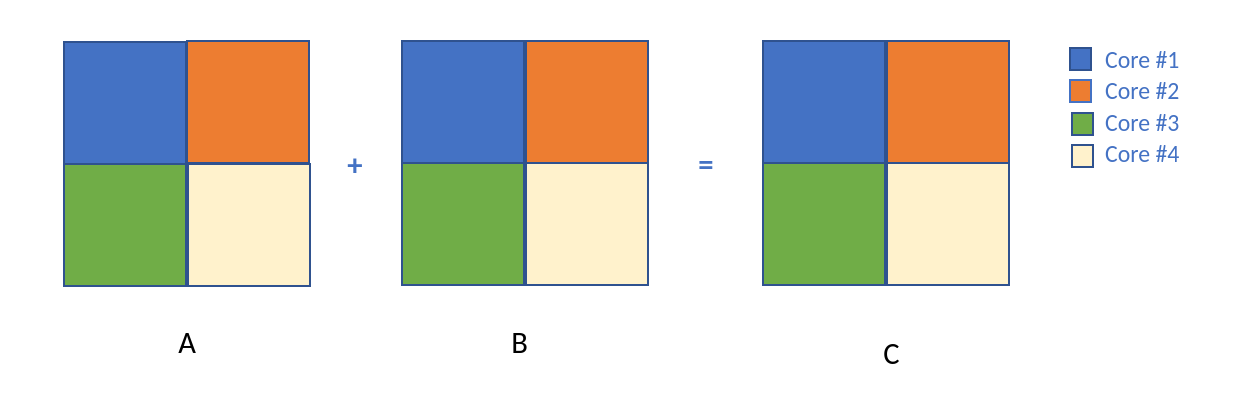
\includegraphics[width=0.72\linewidth]{images/old_backend.png}
			\caption{An example of how C=A+B is performed in parallel in Blaze with 4 cores}	
		\end{figure}	

	\end{outline}
\end{frame}

%\begin{frame}{Background}
%	\begin{outline}
%		\1 Effect of Task Granularity on execution time
%		\1 Universal Scalibility Law
%	\end{outline}
%\end{frame}
\begin{frame}{Loop Scheduling}
	\begin{outline}
			\begin{figure}[]
			\centering
			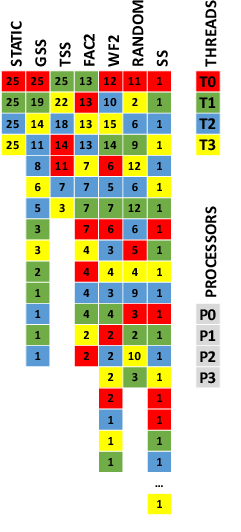
\includegraphics[scale=0.5]{images/loop_cropped.png}
			\caption{An example of loop chunking\footnote{Ciorba, Florina M., Christian Iwainsky, and Patrick Buder. "OpenMP loop scheduling revisited: making a case for more schedules." International Workshop on OpenMP. Springer, Cham, 2018.}}	
			\label{fig_loop}
		\end{figure}
		Chunk size: Number of loop iterations executed by one thread 
		\1Static
		\1Dynamic
		\1Other methods including Guided, Factoring
	\end{outline}
\end{frame}

%\begin{frame}{HPX Tasks}
%	\begin{outline}
%		
%	\end{outline}
%\end{frame}

\begin{frame}{Task Granularity}
	\begin{outline}
		Grain size: The amount of work performed by one HPX thread
		\1What causes performance degradation?
		\2Overheads
		\2Starvation
		\begin{figure}
			\centering
			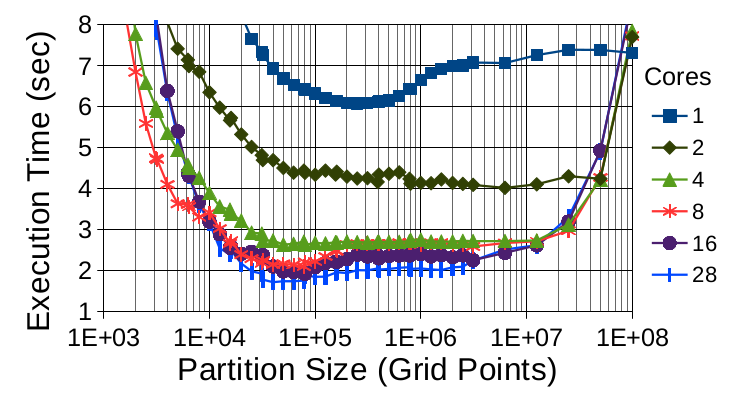
\includegraphics[width=0.72\linewidth]{images/task_granularity.png}
			\caption{The effect of task size on execution time for Stencil application\footnote{Grubel, Patricia, et al. "The performance implication of task size for applications on the hpx runtime system." 2015 IEEE International Conference on Cluster Computing. IEEE, 2015.}}	
	
		\end{figure}
		
	\end{outline}
\end{frame}


\begin{frame}{Modeling Performance}
	\begin{outline}
		\1Amdahl's Law
			$$S(p) = \frac{p}{1+\sigma(p-1)}$$
		\1Universal Scalibility Law
		$$X(p) = \frac{\gamma{p}}{1+\sigma(p-1)+\kappa{p}(p-1)}$$
		\2 Models the effects
		of linear speedup, contention delay, and coherency delay due to crosstalk
		\begin{figure}[H]
			\centering
			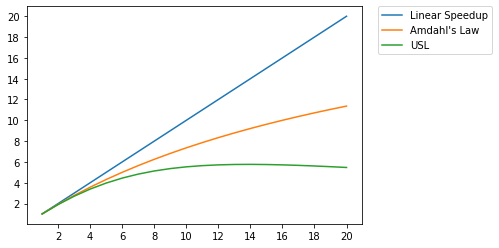
\includegraphics[scale=0.4]{images/amdahls.png}
			\caption{An example of the achievable speedup based on Amdahl's law and USL compared to the ideal linear speedup where $\sigma=0.04$ and $\kappa=0.005$.}	
			\label{fig_Amdahl}
		\end{figure}
		

	\end{outline}
\end{frame}

\begin{frame}{Modeling Performance: Other Models}
	\begin{outline}
		\1Quadratic model
		$$ S(p) = p-\gamma{p(p-1)}$$
		\1Exponential model
		$$S(p) = p(1-\alpha)^{(p-1)}$$
		\1Geometric model
		$$S(p) = \frac{1-\phi^{p}}{1-\phi}$$
	\end{outline}
\end{frame}

\begin{frame}{Objective}
	\begin{outline}
		Dynamically divide the work among the cores based on number of cores, matrix size, complexity of the operation, machine architecture.
		For this purpose two parameters have been introduced:
		\1block\textunderscore size: at each loop iteration the assignment is performed on one block
		\1chunk\textunderscore size: the number of loop iterations included in one task 
		\begin{figure}
			\centering
			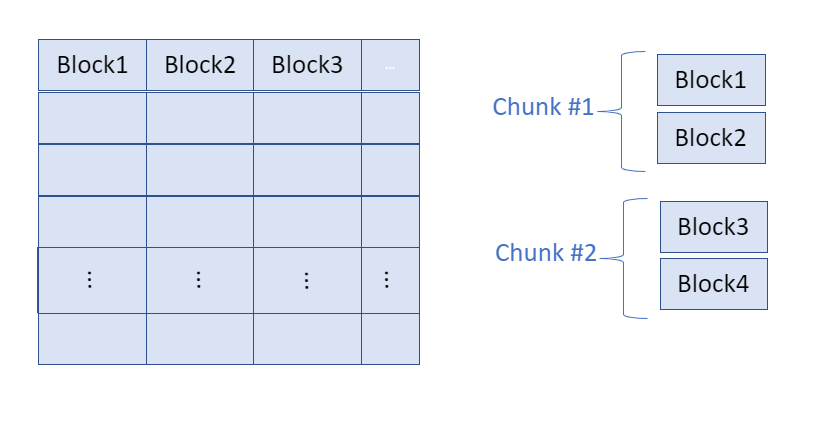
\includegraphics[width=0.72\linewidth]{images/chunks.png}
			\caption{An example of blocking and creating chunks for chunk\textunderscore size = 2}	
		\end{figure}	
	\end{outline}
\end{frame}

%\begin{frame}{Definitions}
%	\begin{outline}
%	\1Block size
%	\1Chunk size
%	\1Grain size
%	\end{outline}
%\end{frame}
\section{Method}
\begin{frame}{Data Collection}
	\begin{outline}
		\1Starting from DMATDMATADD benchmark: $C=A+B$
	\begin{table}[H]
		\centering
		\resizebox{\textwidth}{!}
		{\begin{tabular}{|c | c |} 
				\hline
				Category & Configuration \\
				\hline
				\hline
				Matrix sizes & 200, 230, 264, 300, 396, 455, 523, 600, 690, 793, 912, 1048, 1200, 1380, 1587 \\ [0.5ex] 
				\hline
				Number of cores & 1, 2, 3, 4, 5, 6, 7, 8 \\ 	
				\hline
				Number of rows in the block & 4, 8, 12, 16, 20, 32 \\
				\hline	
				Number of columns in the block & 64, 128, 256, 512, 1024 \\
				\hline
				Chunk size & Between 1 and total number of blocks (logarithmic increase)\\\hline
		\end{tabular}}
		
		\caption{List of different values used for each variable for running the $DMATDMATADD$ benchmark}
		\label{table1}
	\end{table}
	\end{outline}
\end{frame}


\begin{frame}{Data}
	\begin{outline}
		\1For simplicity we look at each matrix size individually, one number of core at a time, 
		
		
		\begin{figure}
			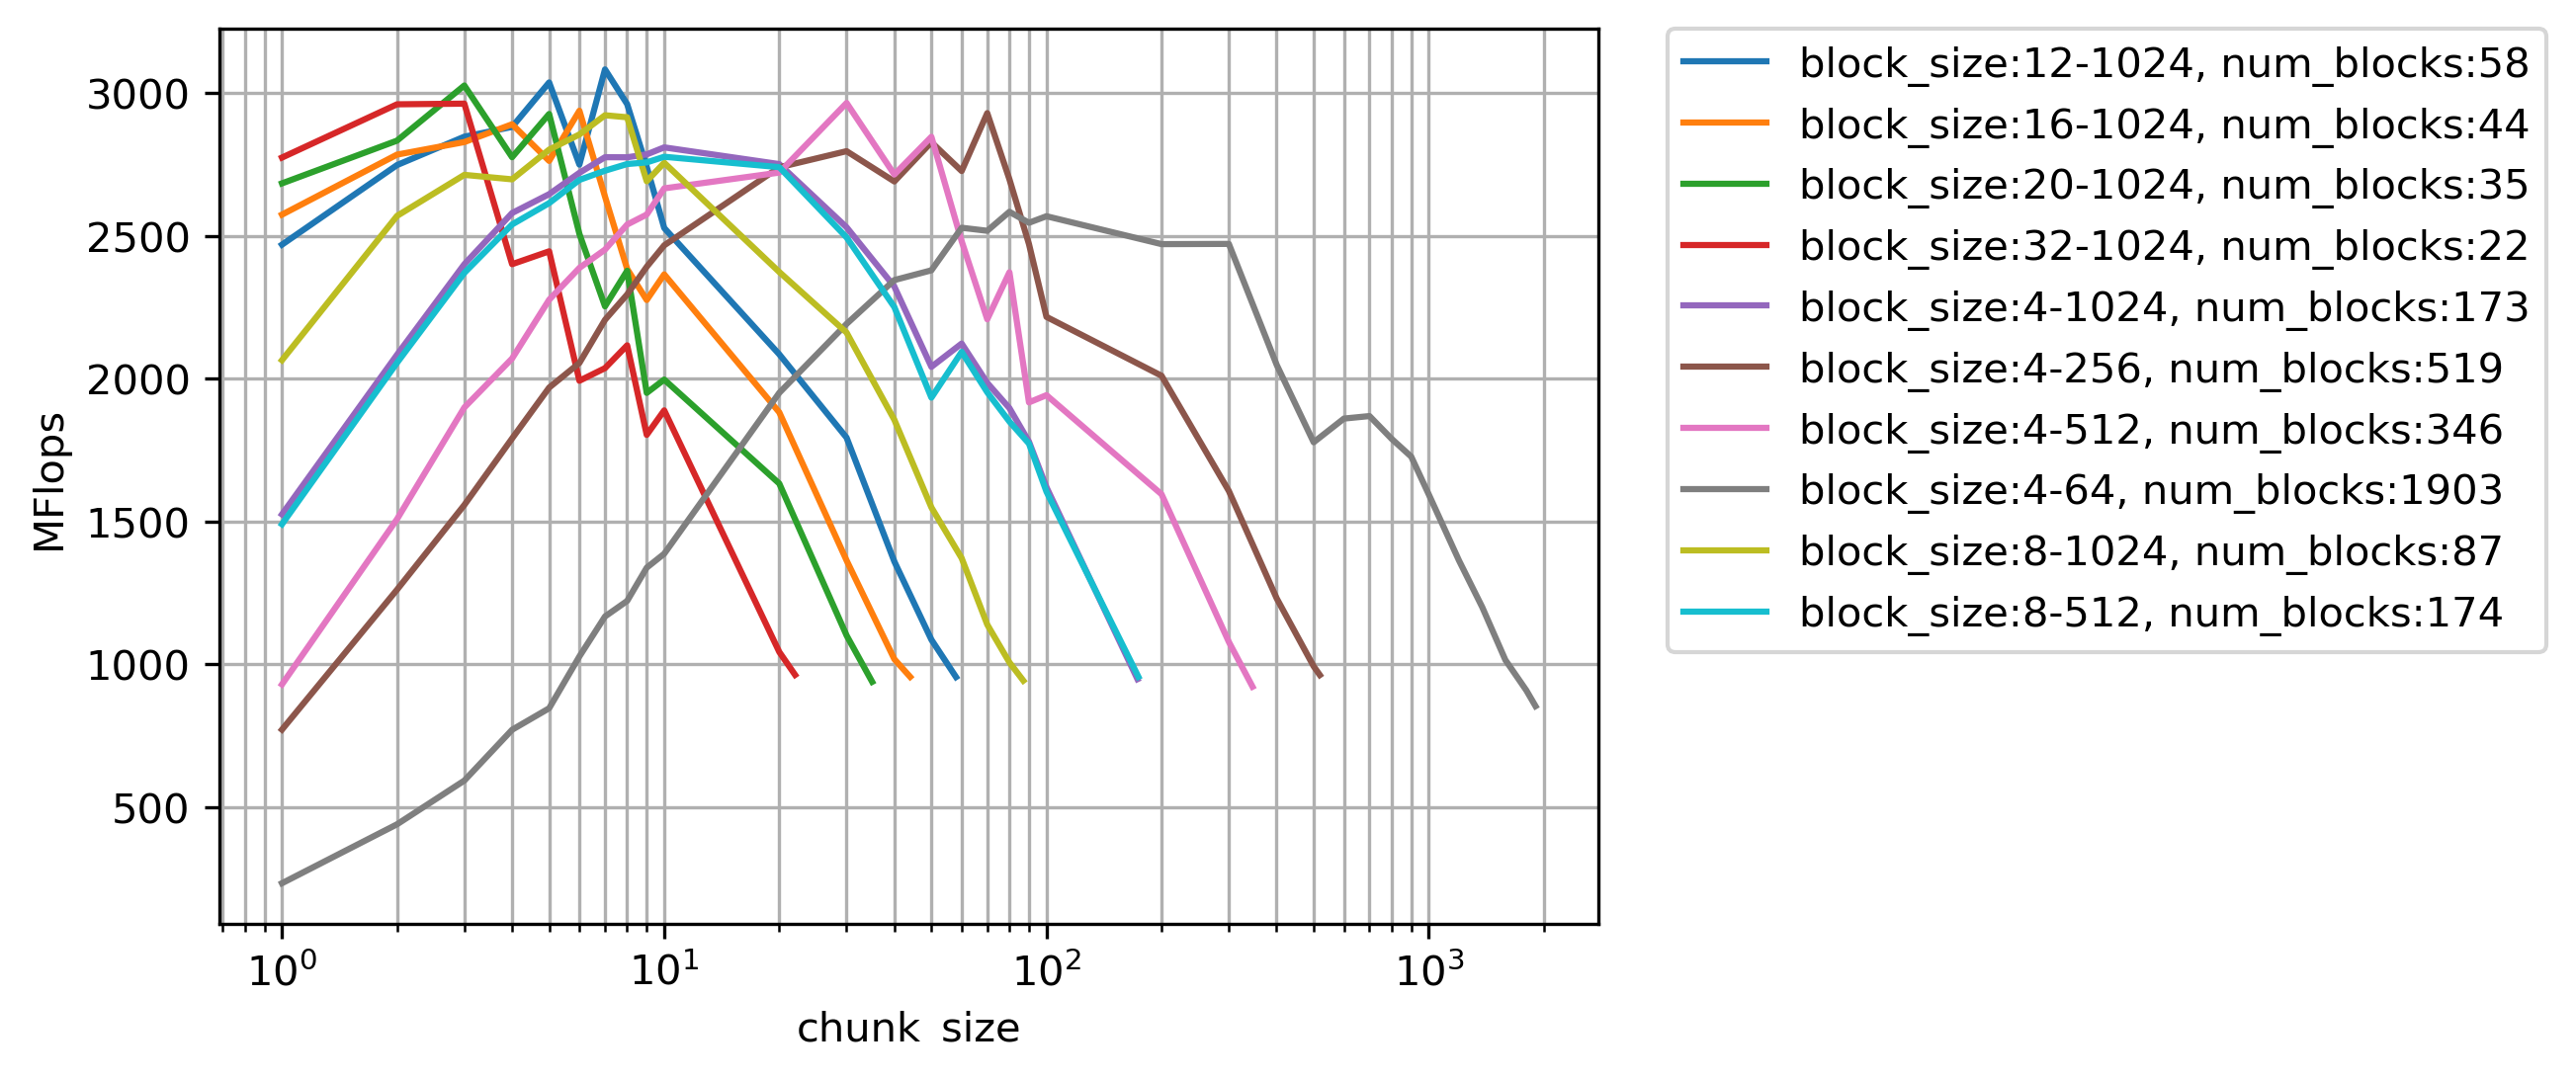
\includegraphics[width=0.9\linewidth]{images/fig5.png}	
			\caption{The results obtained from running $DMATDMATADD$ benchmark through Blazemark for matrix sizes from 690$\times$690 with different combinations of block size and chunk size on $4$ cores}	
		\end{figure}
	\end{outline}
\end{frame}


\begin{frame}{Observation}
	\begin{outline}
		\begin{figure}
			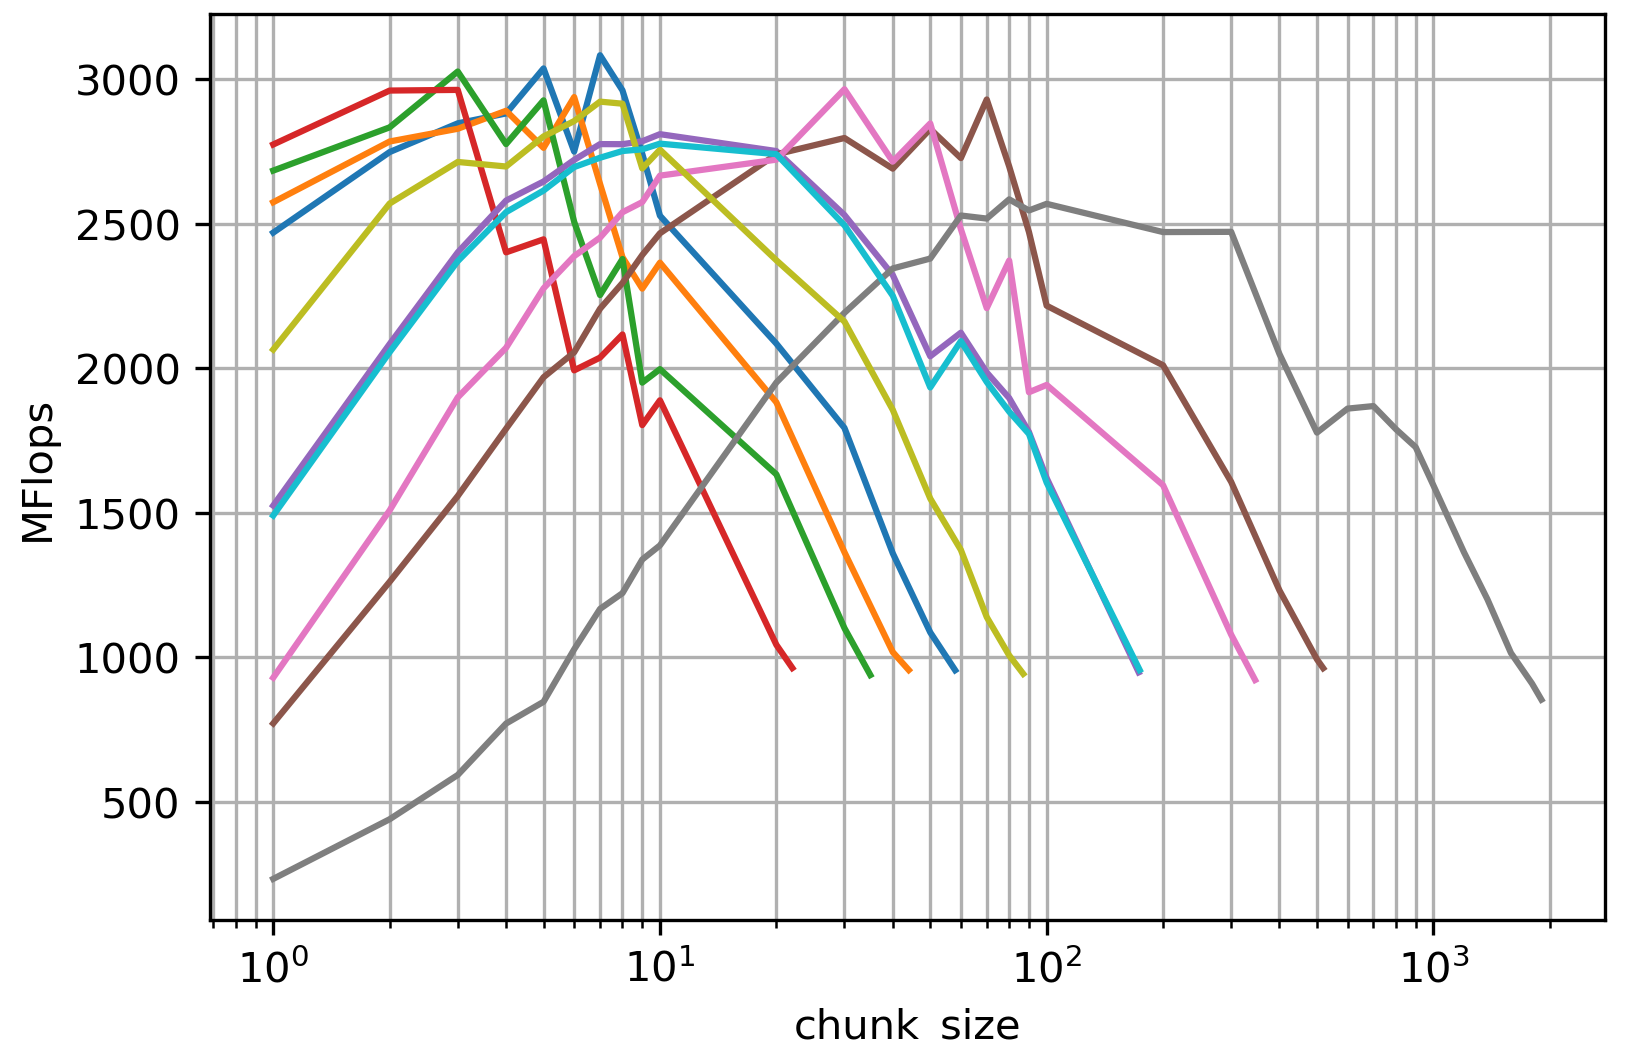
\includegraphics[scale=0.2]{images/fig5_cropped.png}			
		\end{figure}
		\1For each selected block size, there is a range of chunk sizes that gives us the best performance. 
		\1Except for some uncommon cases, no matter which block size we choose, we are able to achieve the maximum performance if we select the right chunk size.  
	\end{outline}
\end{frame}

\begin{frame}{Throughput vs. Grain Size}
	\begin{outline}
		Grain size: The amount of work performed by one HPX thread
		
		\begin{figure}[H]
			\centering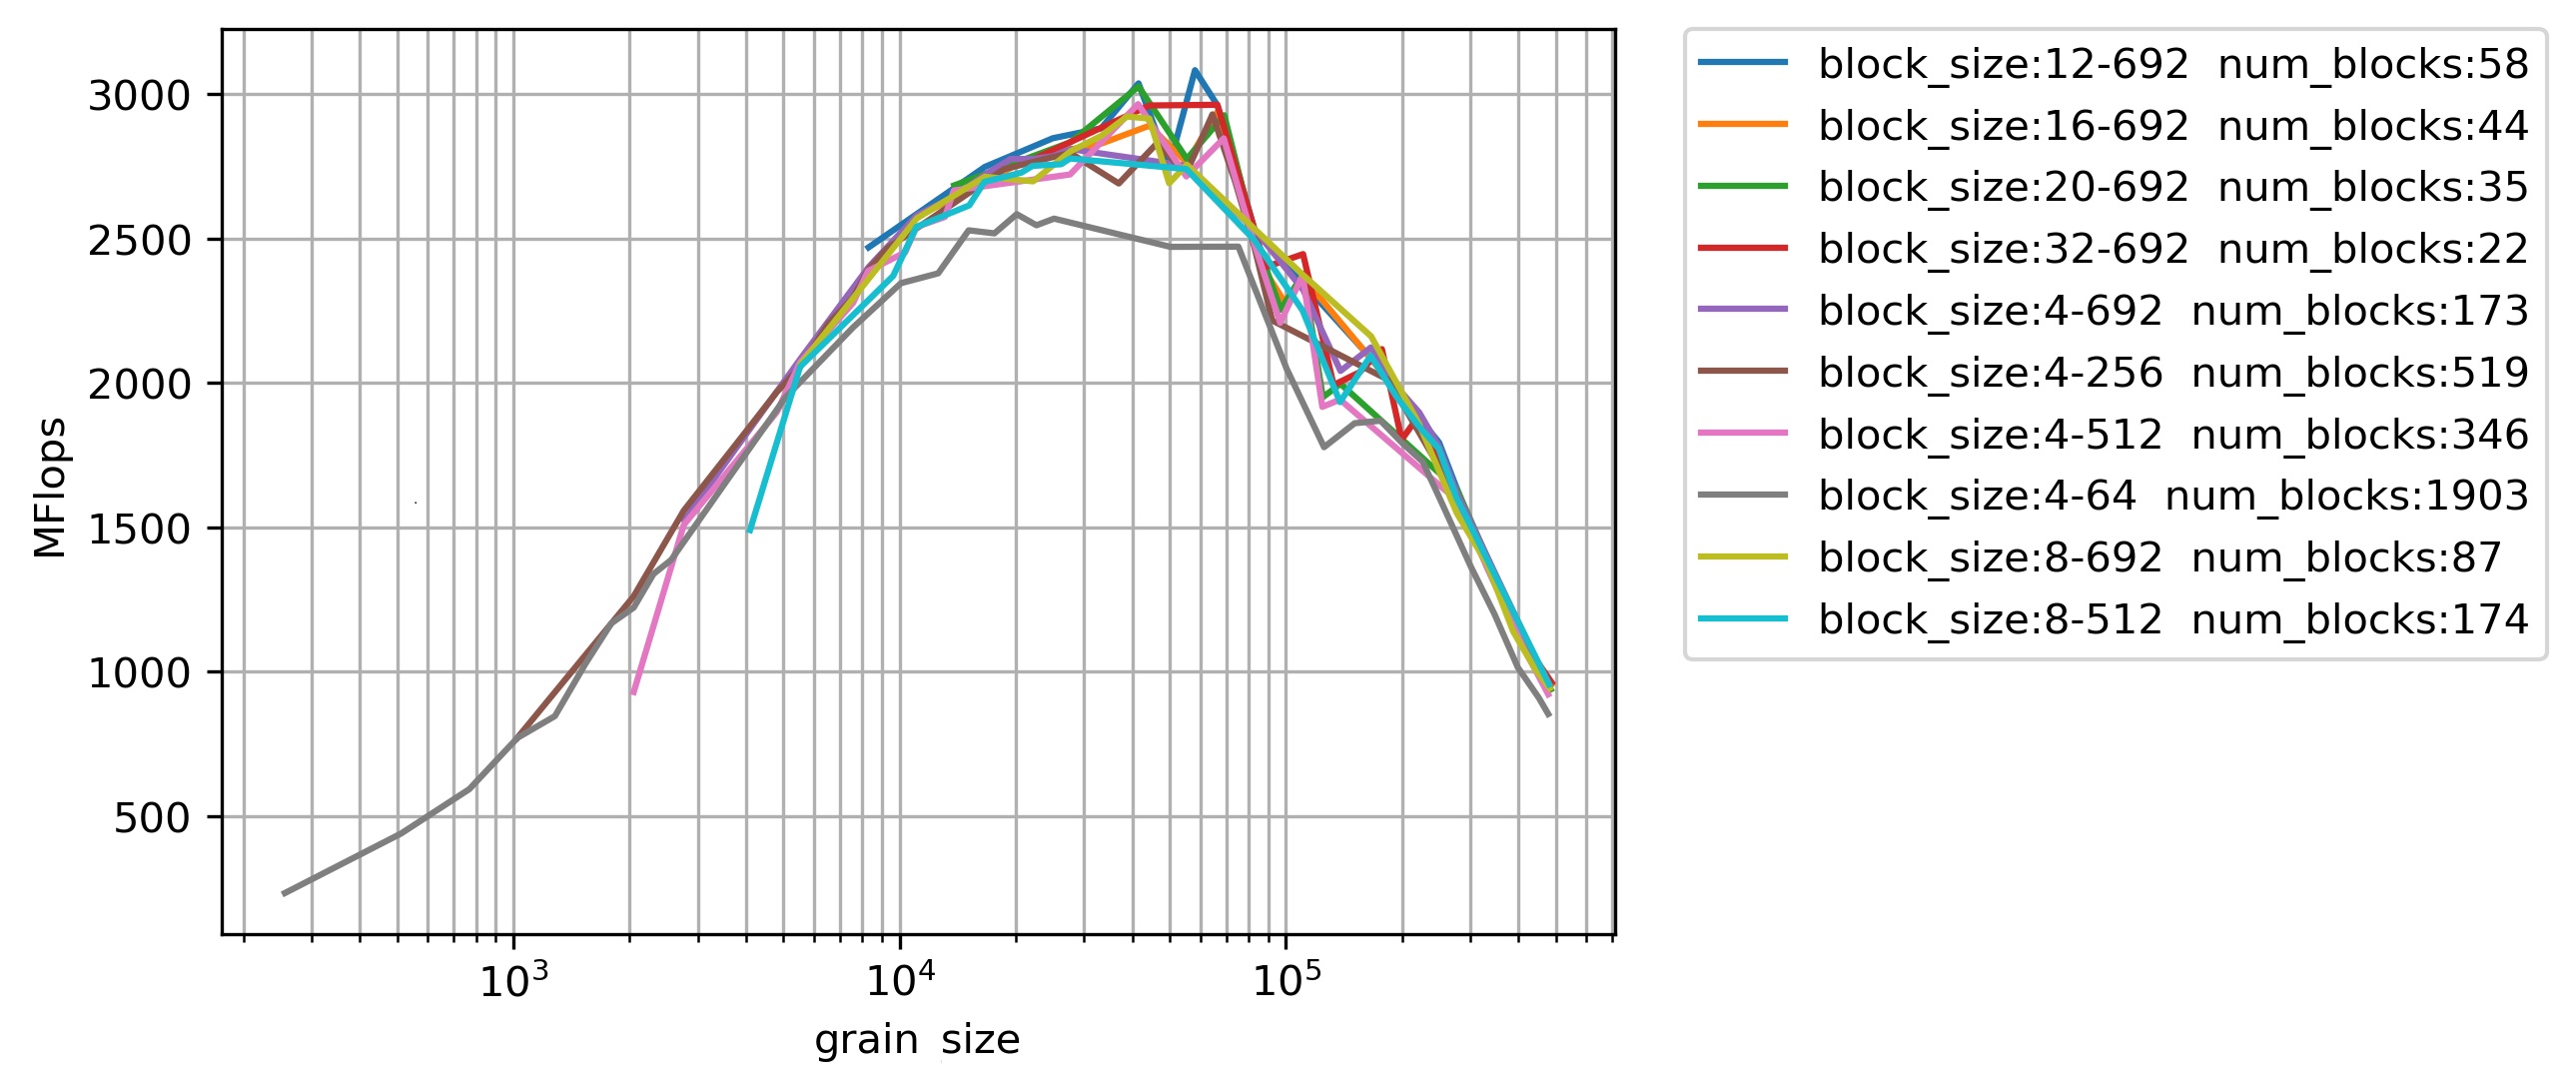
\includegraphics[width=1\linewidth]{images/fig6.png}
			\caption{The results obtained from running $DMATDMATADD$ benchmark through Blazemark for matrix size 690$\times$690 on $4$ cores.}	
			\label{fig6}
		\end{figure}
	
	\end{outline}
\end{frame}

\begin{frame}{Throughput vs. Grain Siz}
	\begin{outline}
		Can we model the relationship between the throughput and the grain size?
	\end{outline}
\end{frame}

\begin{frame}{Modeling}
	\begin{outline}
		1- Polynomial Model
		
		
				\vspace{\baselineskip}
		2- Bathtub Model
	\end{outline}
\end{frame}

\begin{frame}{Method: Polynomial Model}
	\begin{outline}
		In order to simplify the process and eliminate the effect of different possible factors, we started with limiting the problem to a fixed matrix size.	
		\1Used a second order polynomial to model the relationship between the throughput and the grain size when number of cores is fixed.
		 $$P=ag^2+bg+c$$    
		 \1Divide the data into training(60\%) and test(40\%)
	\end{outline}
\end{frame}

\begin{frame}{Method: Modeling Performance based on Grain Size}
	\begin{outline}	
		\begin{figure}[H]
			\centering
			{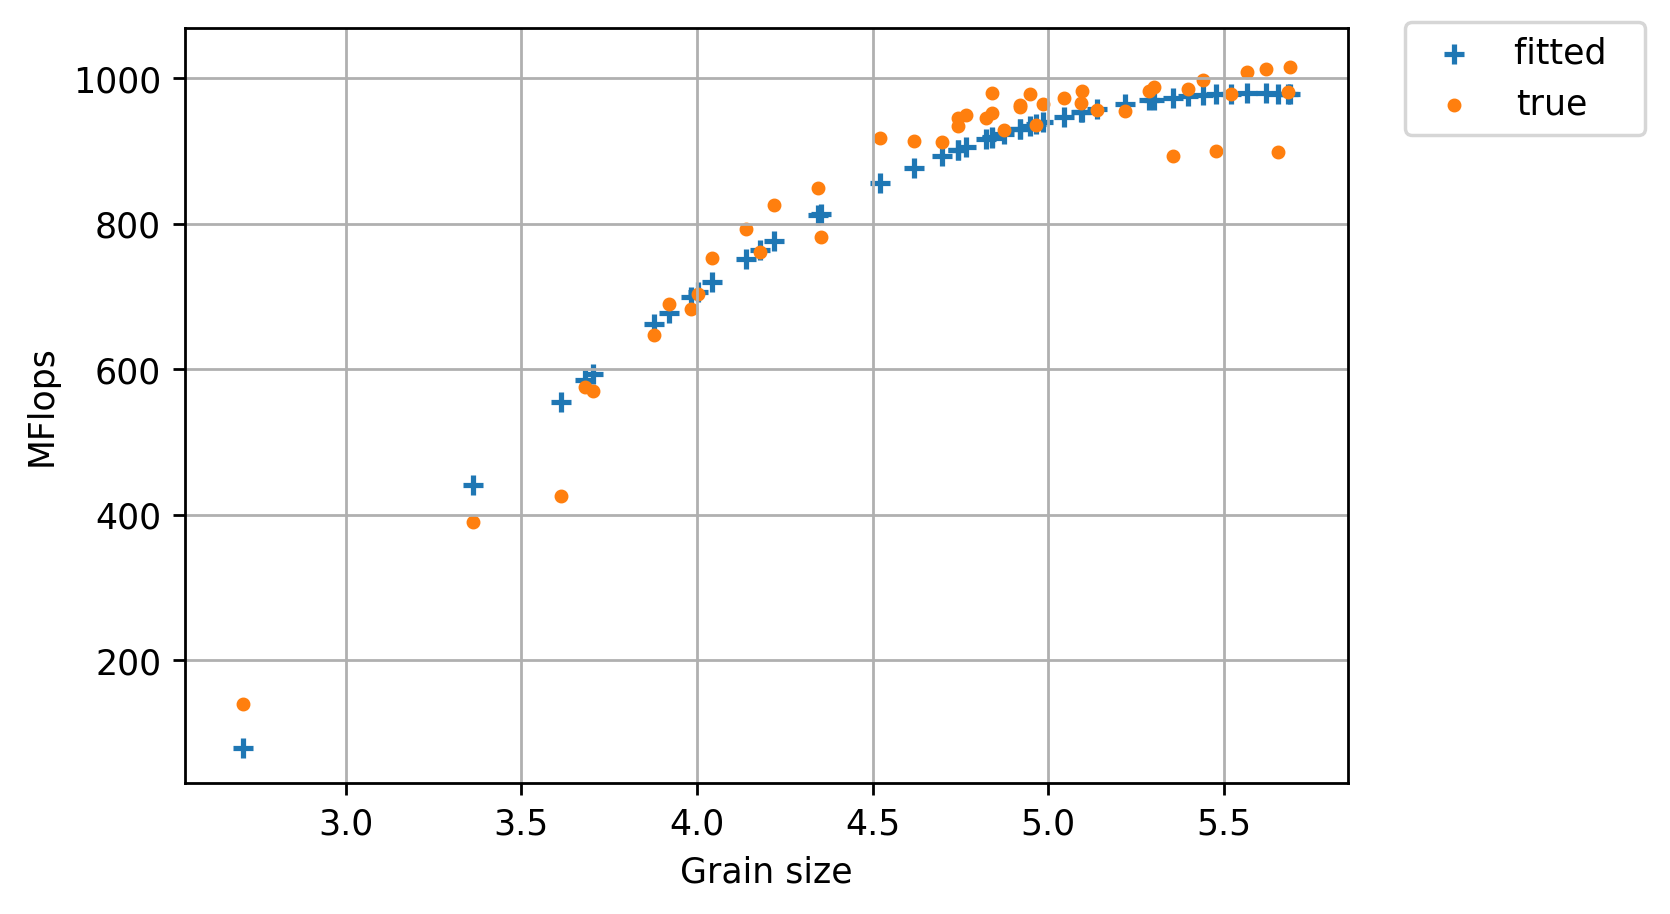
\includegraphics[scale=.2]{images/polyfit/fig_1_690.png}\label{fig10:a}}
			{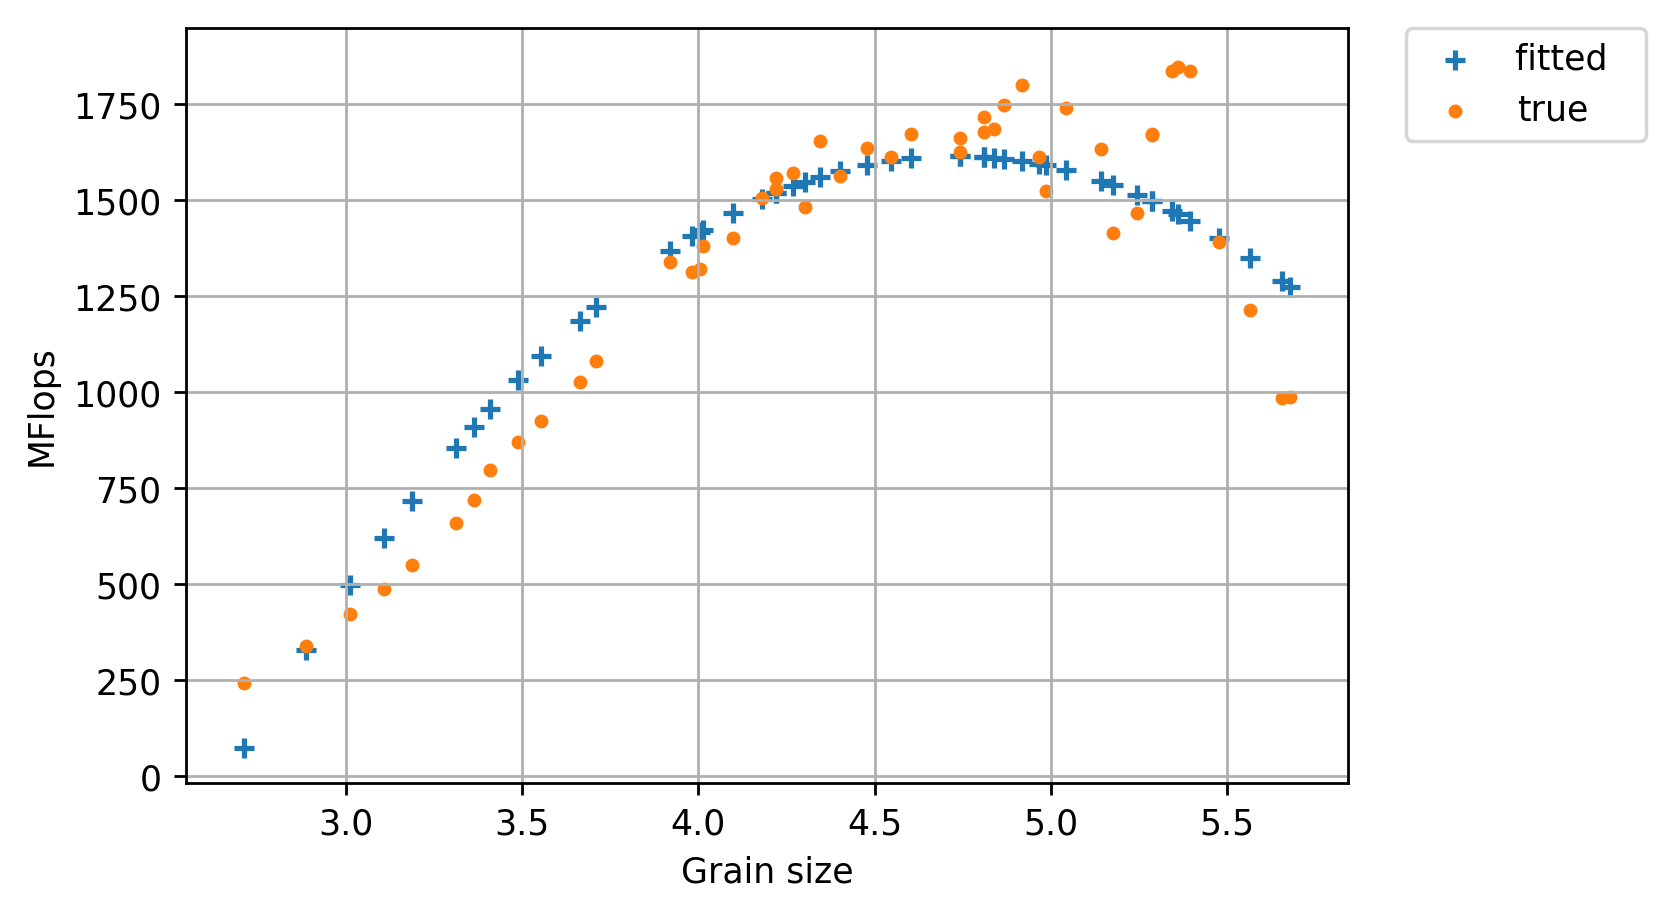
\includegraphics[scale=.2]{images/polyfit/fig_2_690.png}\label{fig10:b}}{\hfill}
			{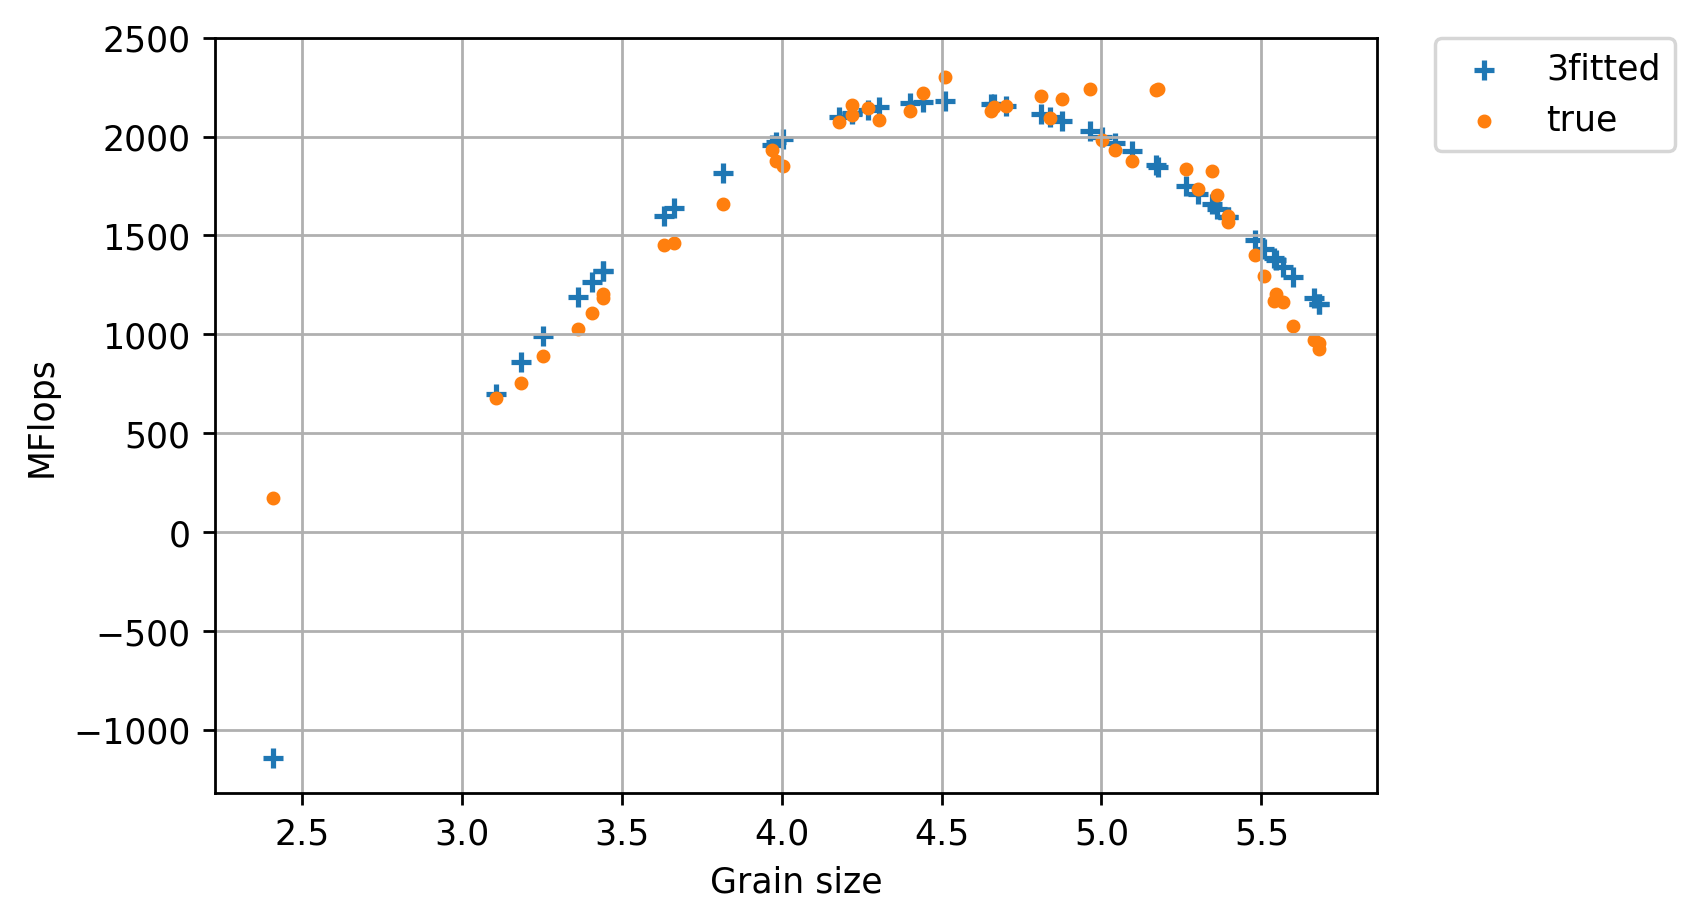
\includegraphics[scale=.2]{images/polyfit/fig_3_690.png}\label{fig10:c}}
			{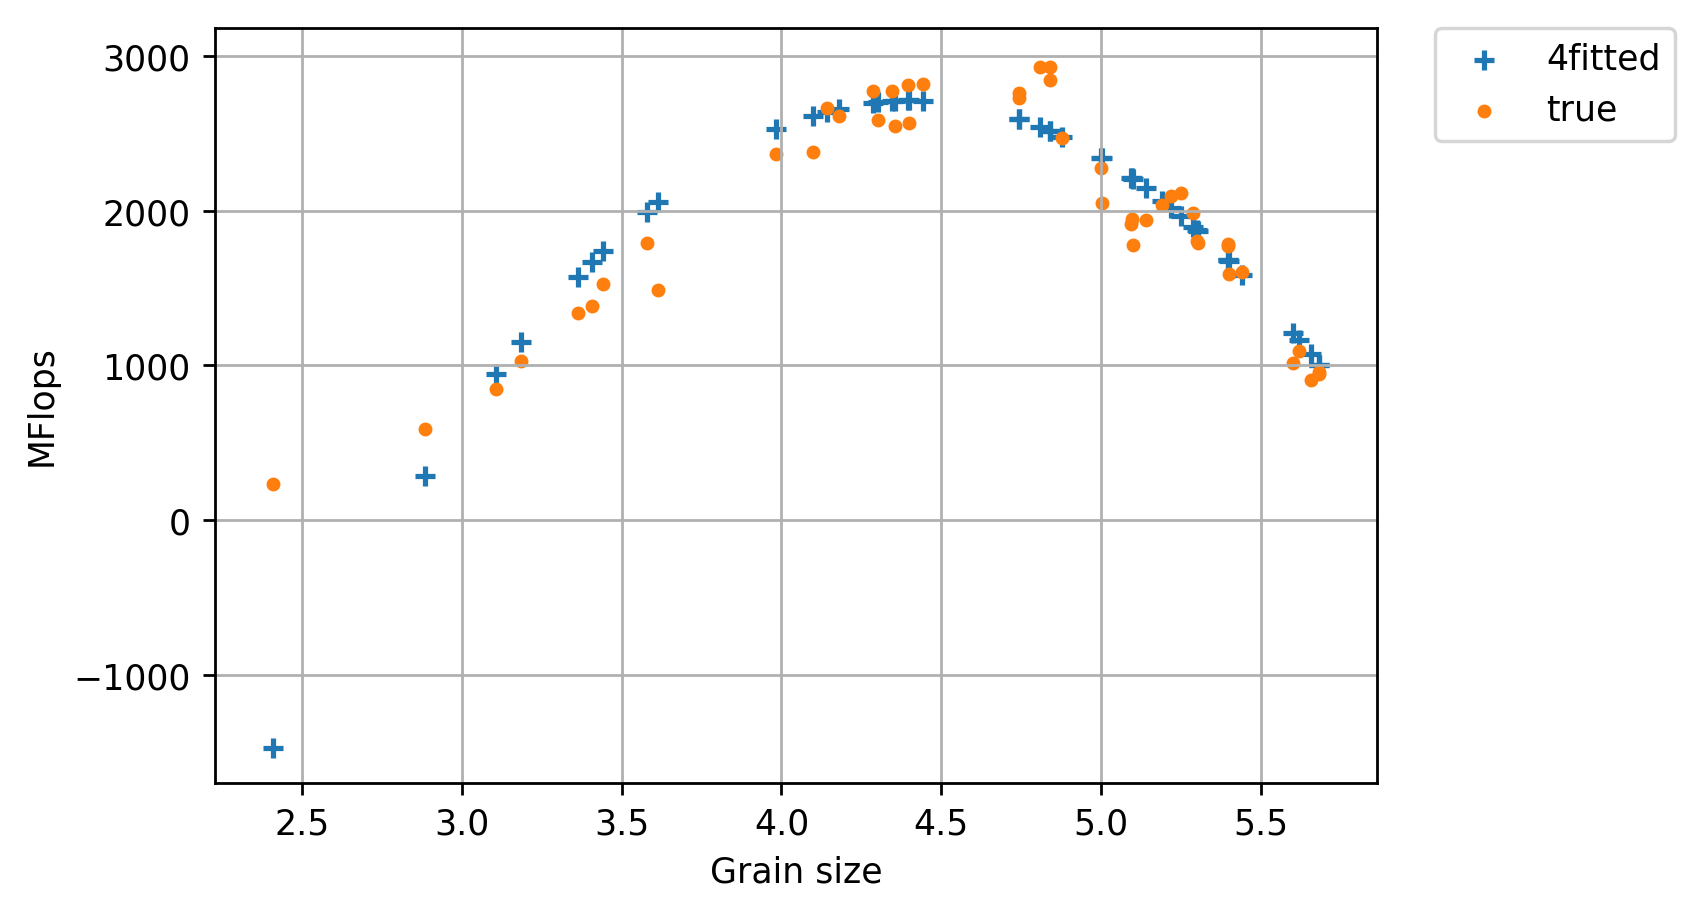
\includegraphics[scale=.2]{images/polyfit/fig_4_690.png}\label{fig10:d}}{\hfill}
			{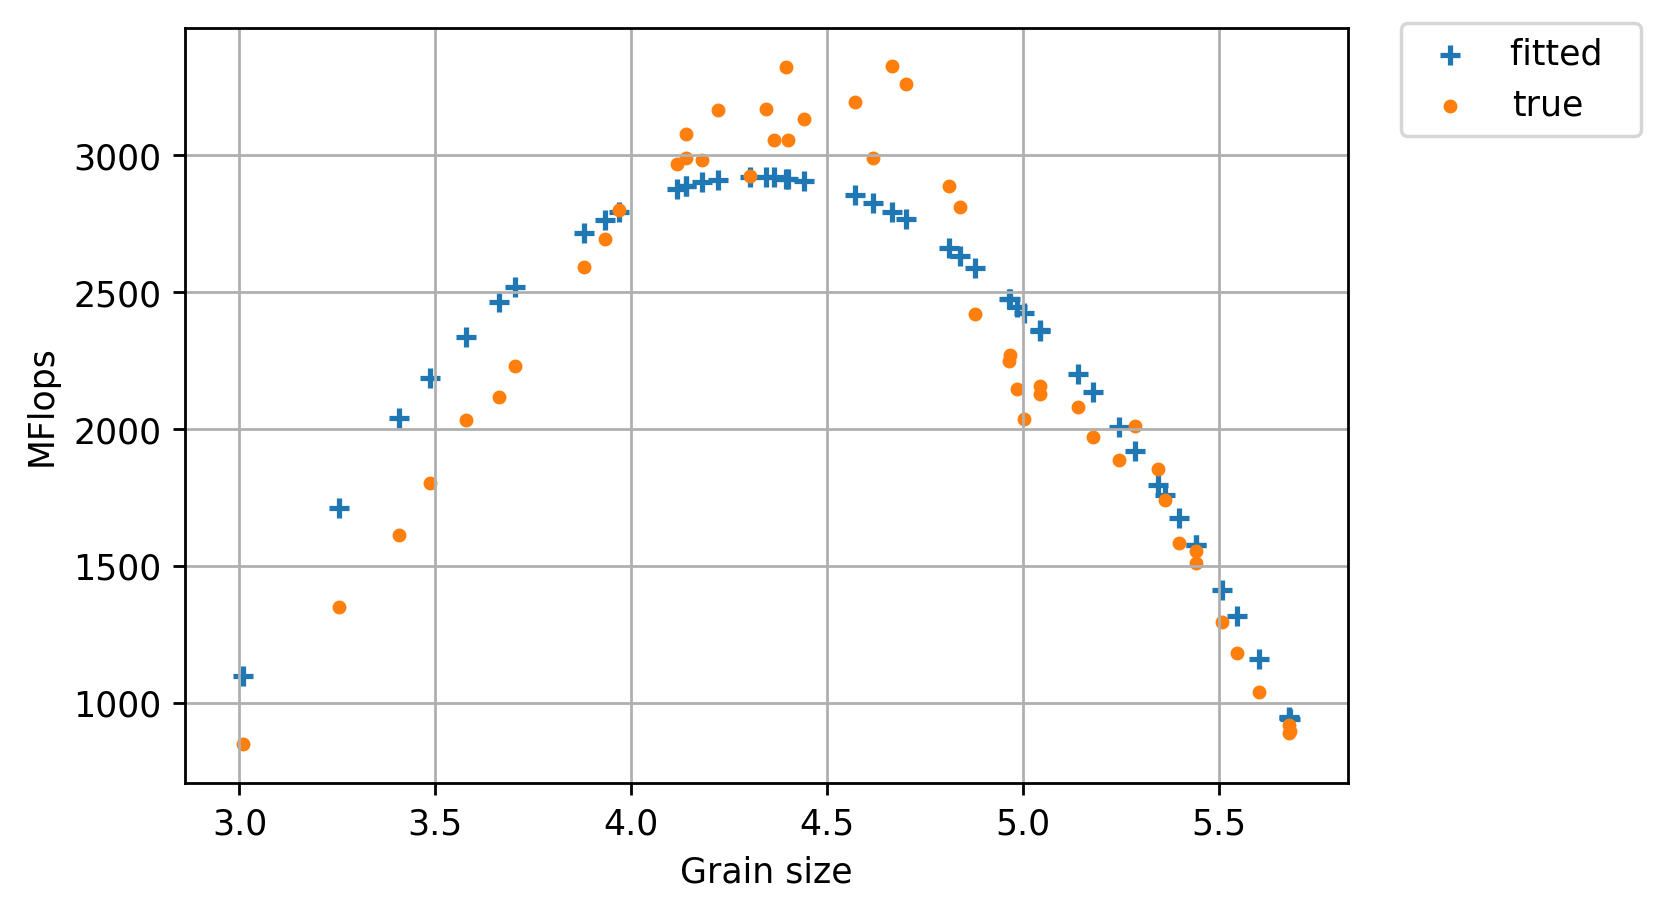
\includegraphics[scale=.2]{images/polyfit/fig_5_690.png}\label{fig10:e}}
			{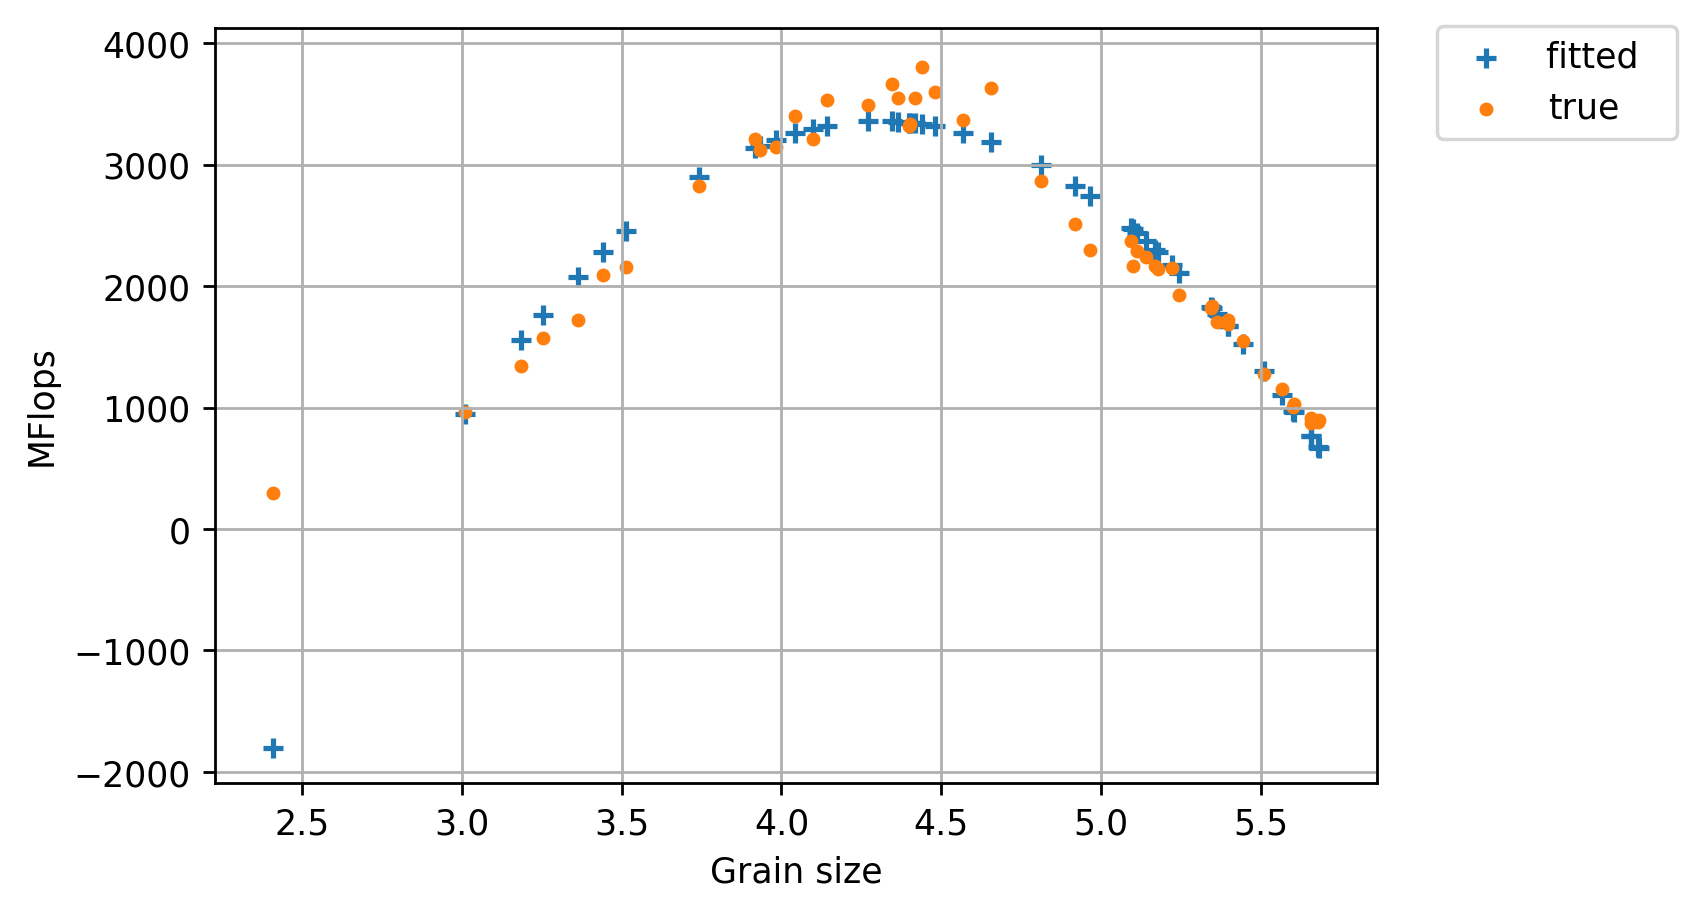
\includegraphics[scale=.2]{images/polyfit/fig_6_690.png}\label{fig10:f}}{\hfill}
			{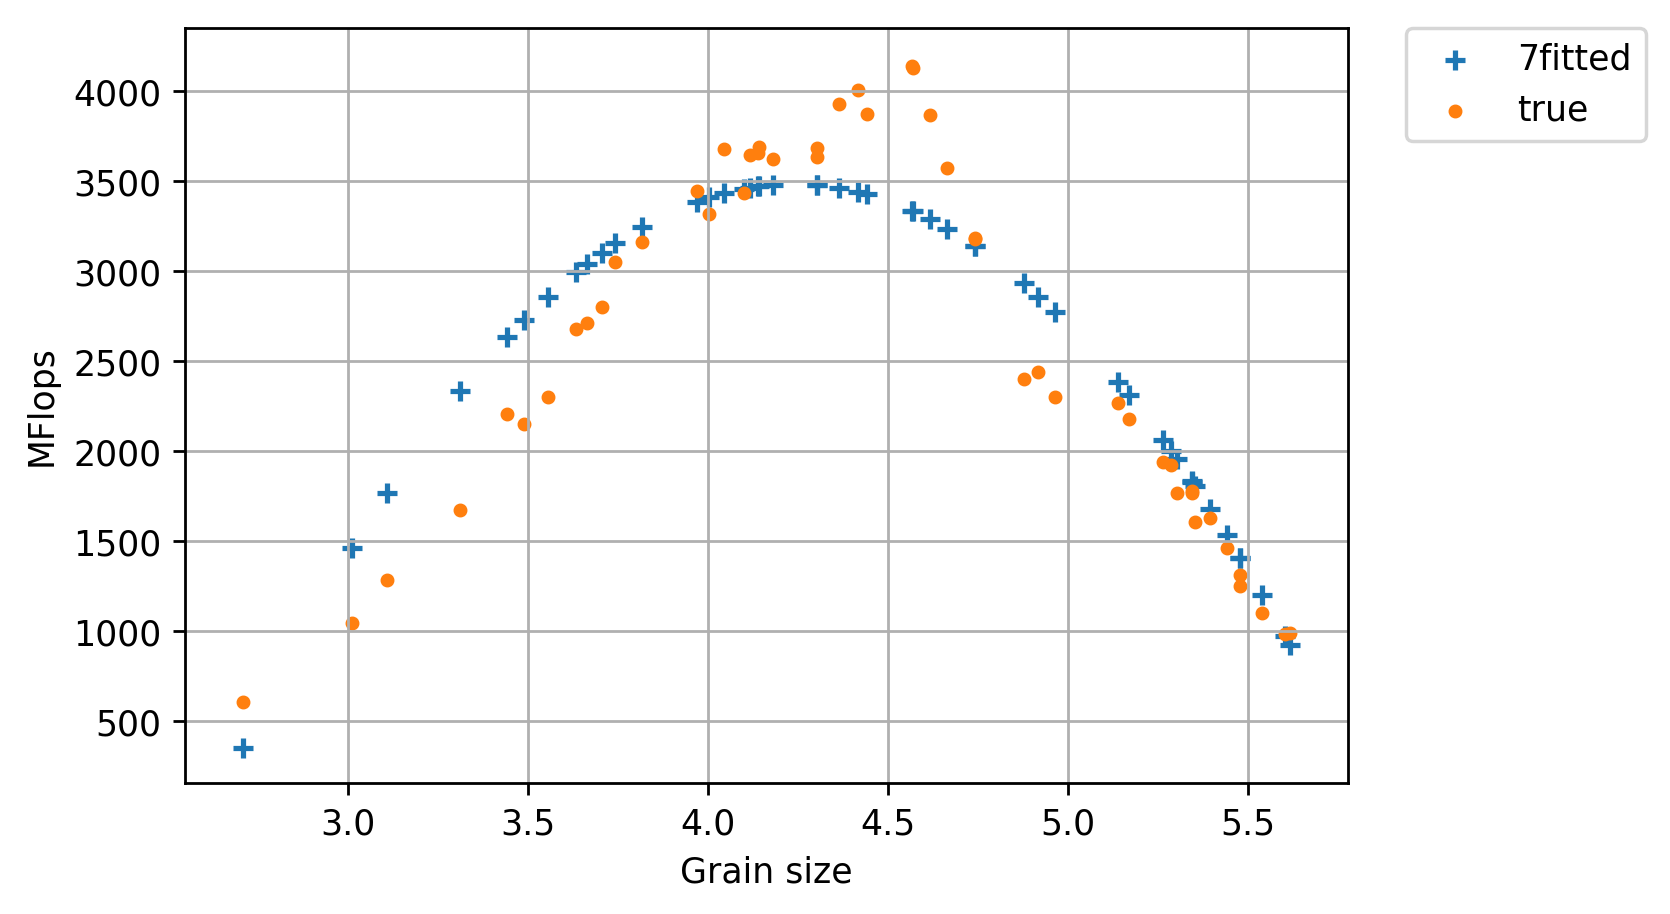
\includegraphics[scale=.2]{images/polyfit/fig_7_690.png}\label{fig10:g}}
			{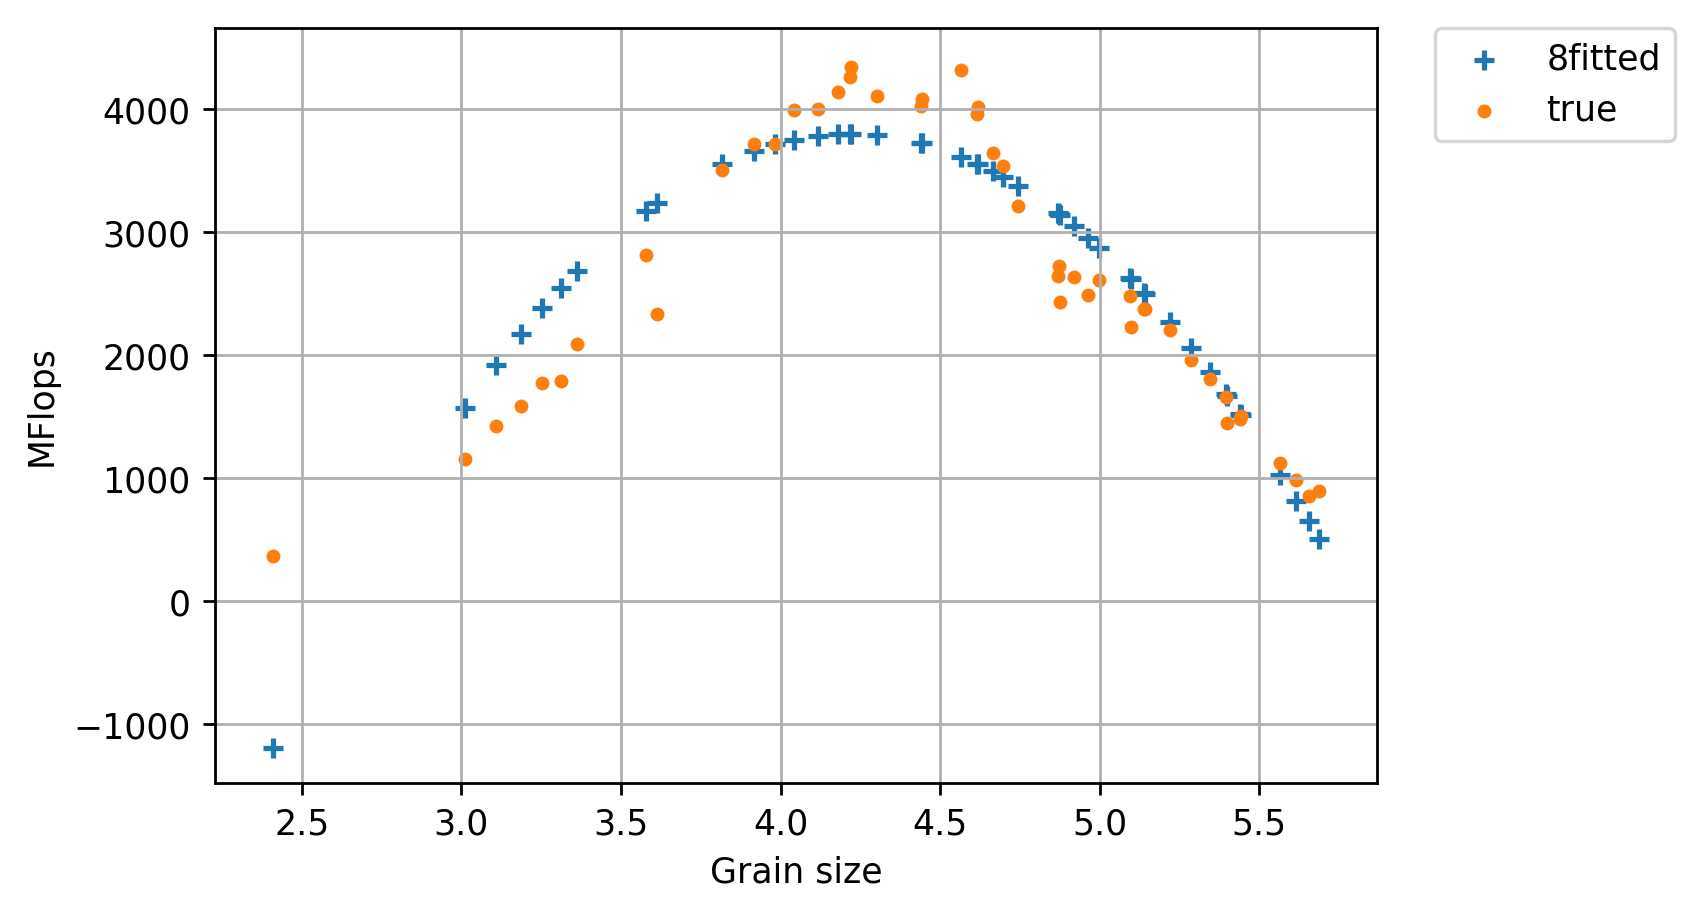
\includegraphics[scale=.2]{images/polyfit/fig_8_690.png}\label{fig10:h}}
			
			\caption{The results of fitting the throughput vs grain size data into a 2d polynomial for $DMATDMATADD$ benchmark for matrix size 690$\times$690 with different number of cores on the test data set (a) 1 core, (b) 2 cores, (c) 3 cores, (d) 4 cores, (e) 5 cores, (f) 6 cores, (g) 7 cores, (h) 8 cores.}	
			\label{fig10}
		\end{figure}
	\end{outline}
\end{frame}


\begin{frame}{Method: Modeling Performance based on Grain Size}
	\begin{outline}	
		$$Relative_error = \frac{1}{n}\sum_{i=1}^{n} {1-p_i/t_i}$$
\begin{figure}[H]
	\centering
	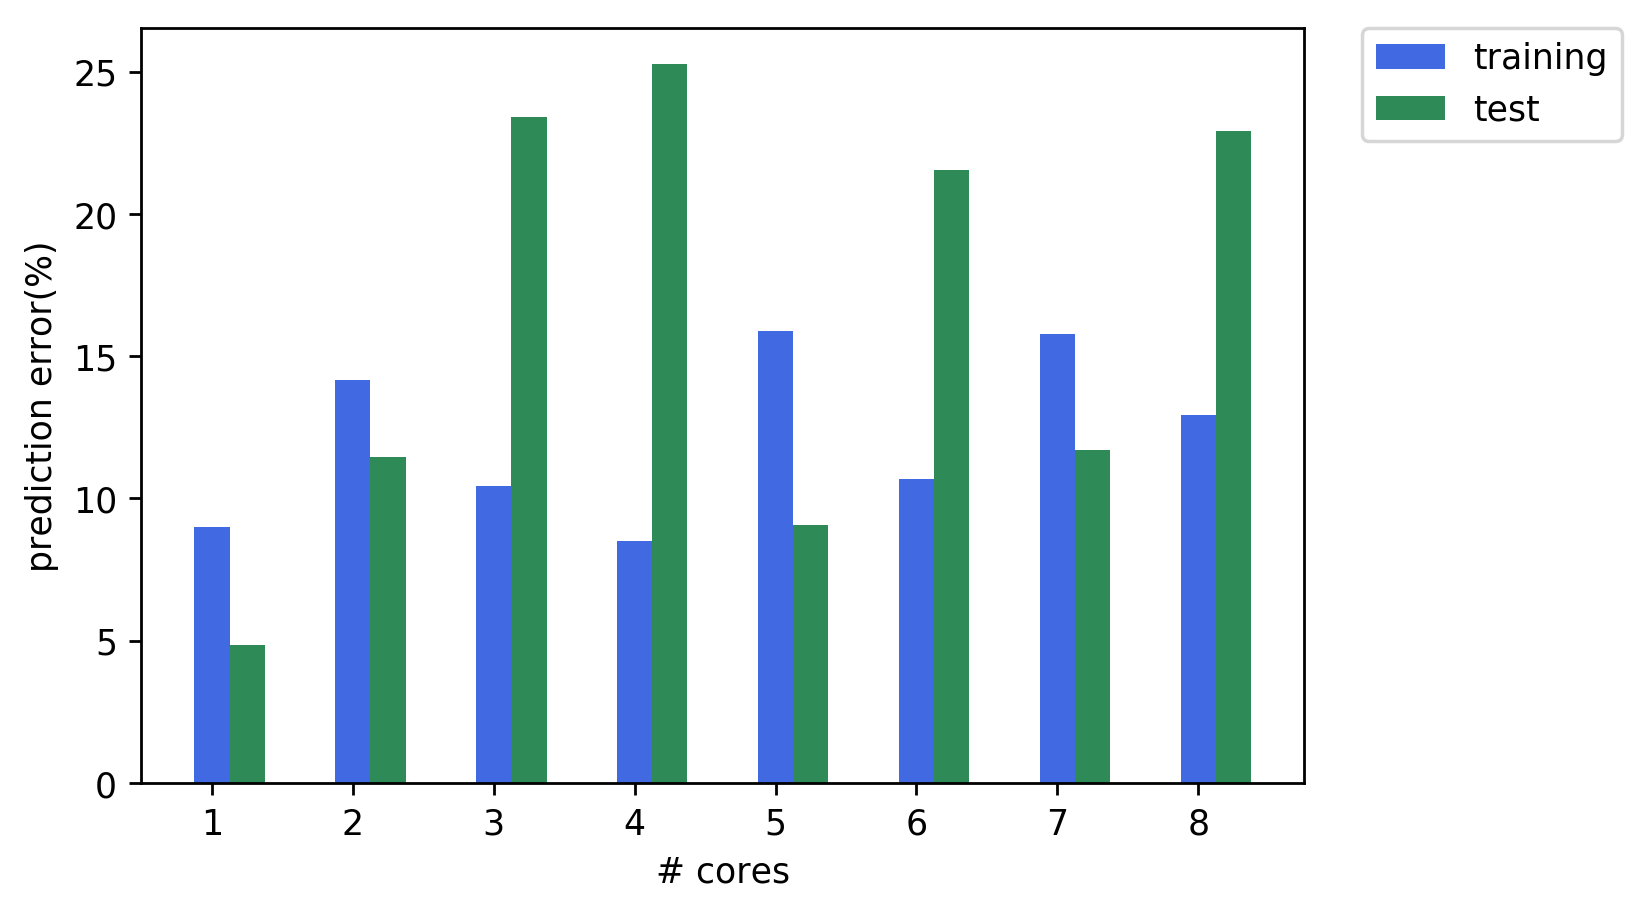
\includegraphics[scale=.5]{images/polyfit/fig_train_test_690.png}
	\caption{The training and test error for fitting data obtained from the $DMATDMATADD$ benchmark for matrix size $690\times690$ against different number of cores cores.}	
	\label{fig11}
\end{figure}
	\end{outline}
\end{frame}

\begin{frame}{Method: Modeling Performance based on Grain Size}
	\begin{outline}	
		Can we somehow integrate number of cores into the model?
	\end{outline}
\end{frame}

\begin{frame}{Method: Modeling Performance based on Grain Size}
	\begin{outline}	
		\1For $P=ag^2+bg+c$, see how $a$, $b$, and $c$ change with the number of cores
		\1Model the relationship with a 3rd degree polynomial
		$$a=a_0N^3+a_1N^2+a_2N+a_3
		,\:b=b_0N^3+b_1N^2+b_2N+b_3,$$ $$c=c_0N^3+c_1N^2+c_2N+c_3$$
		\begin{figure}[H]
			\centering
			{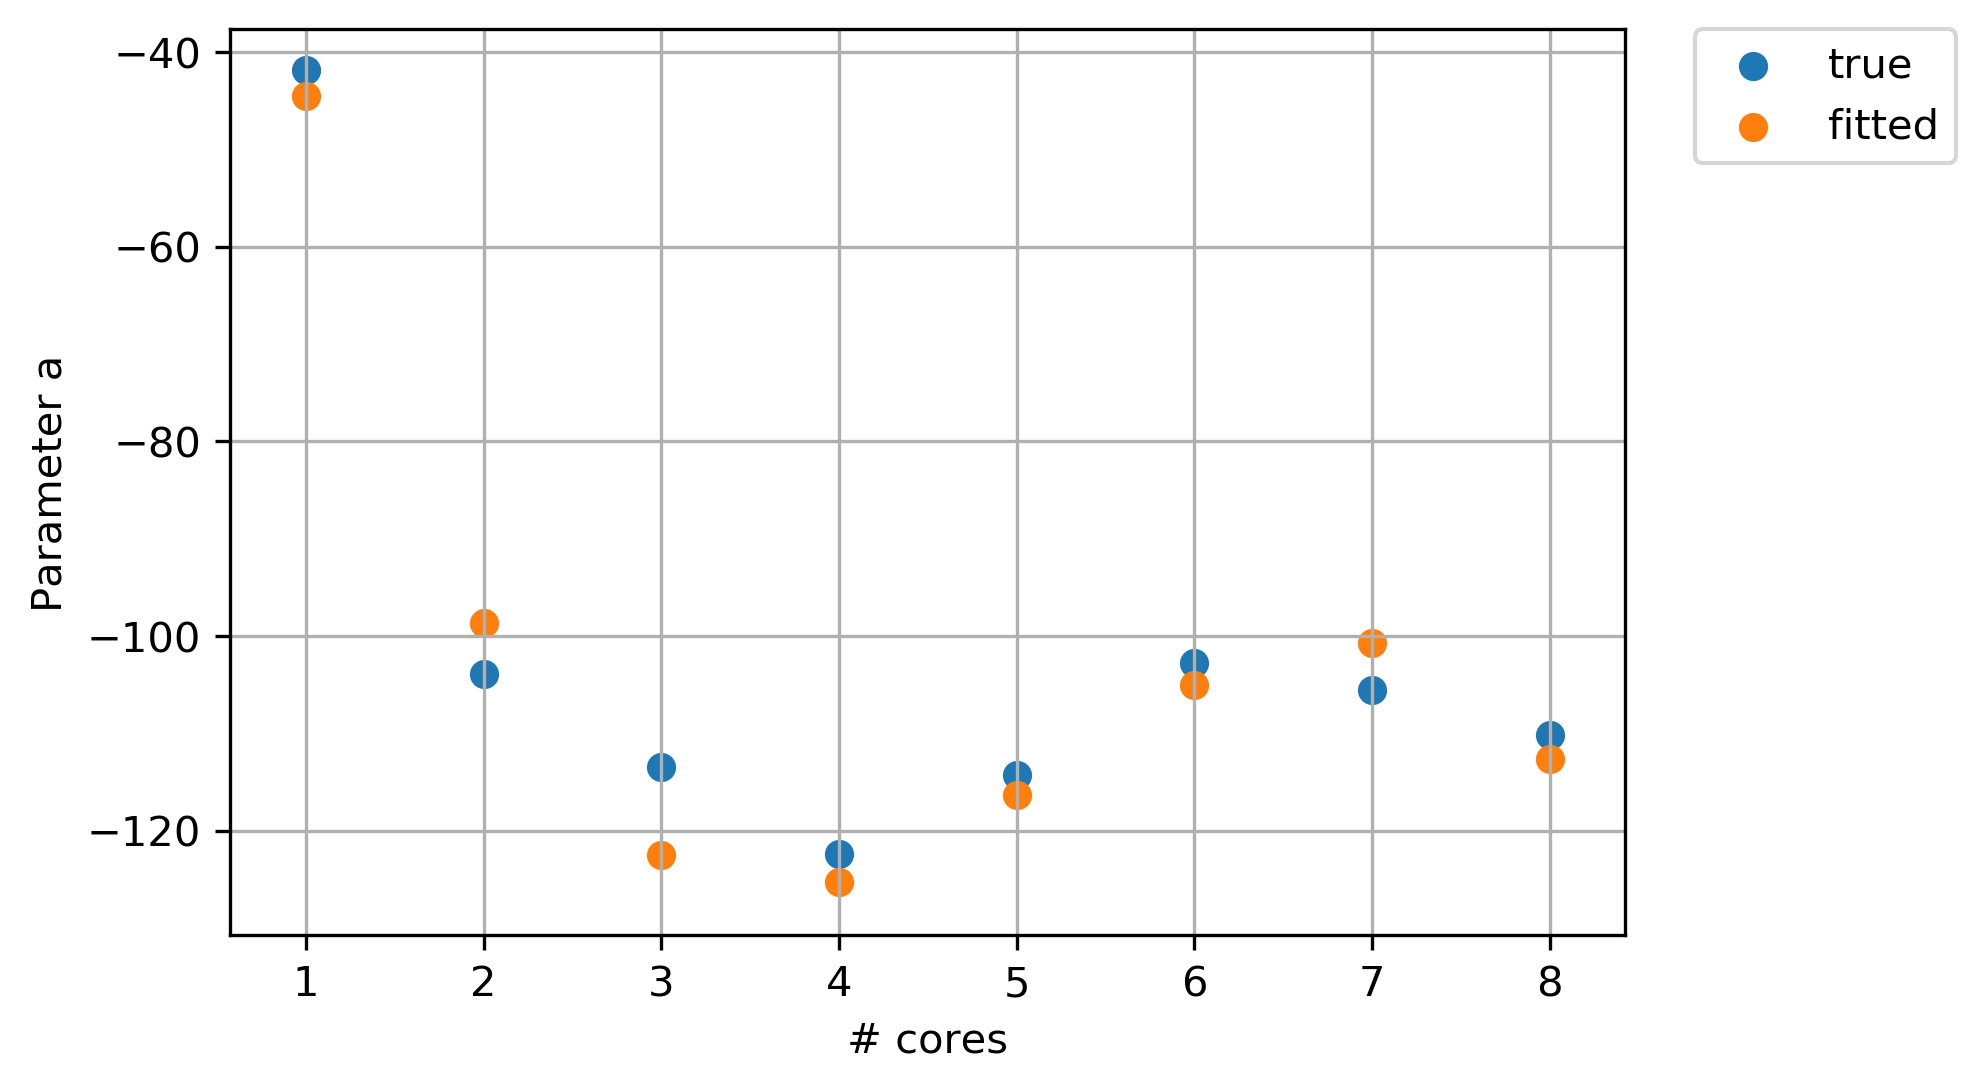
\includegraphics[scale=.2]{images/polyfit/fig_690_params_0.png}\label{fig15:a}}
			{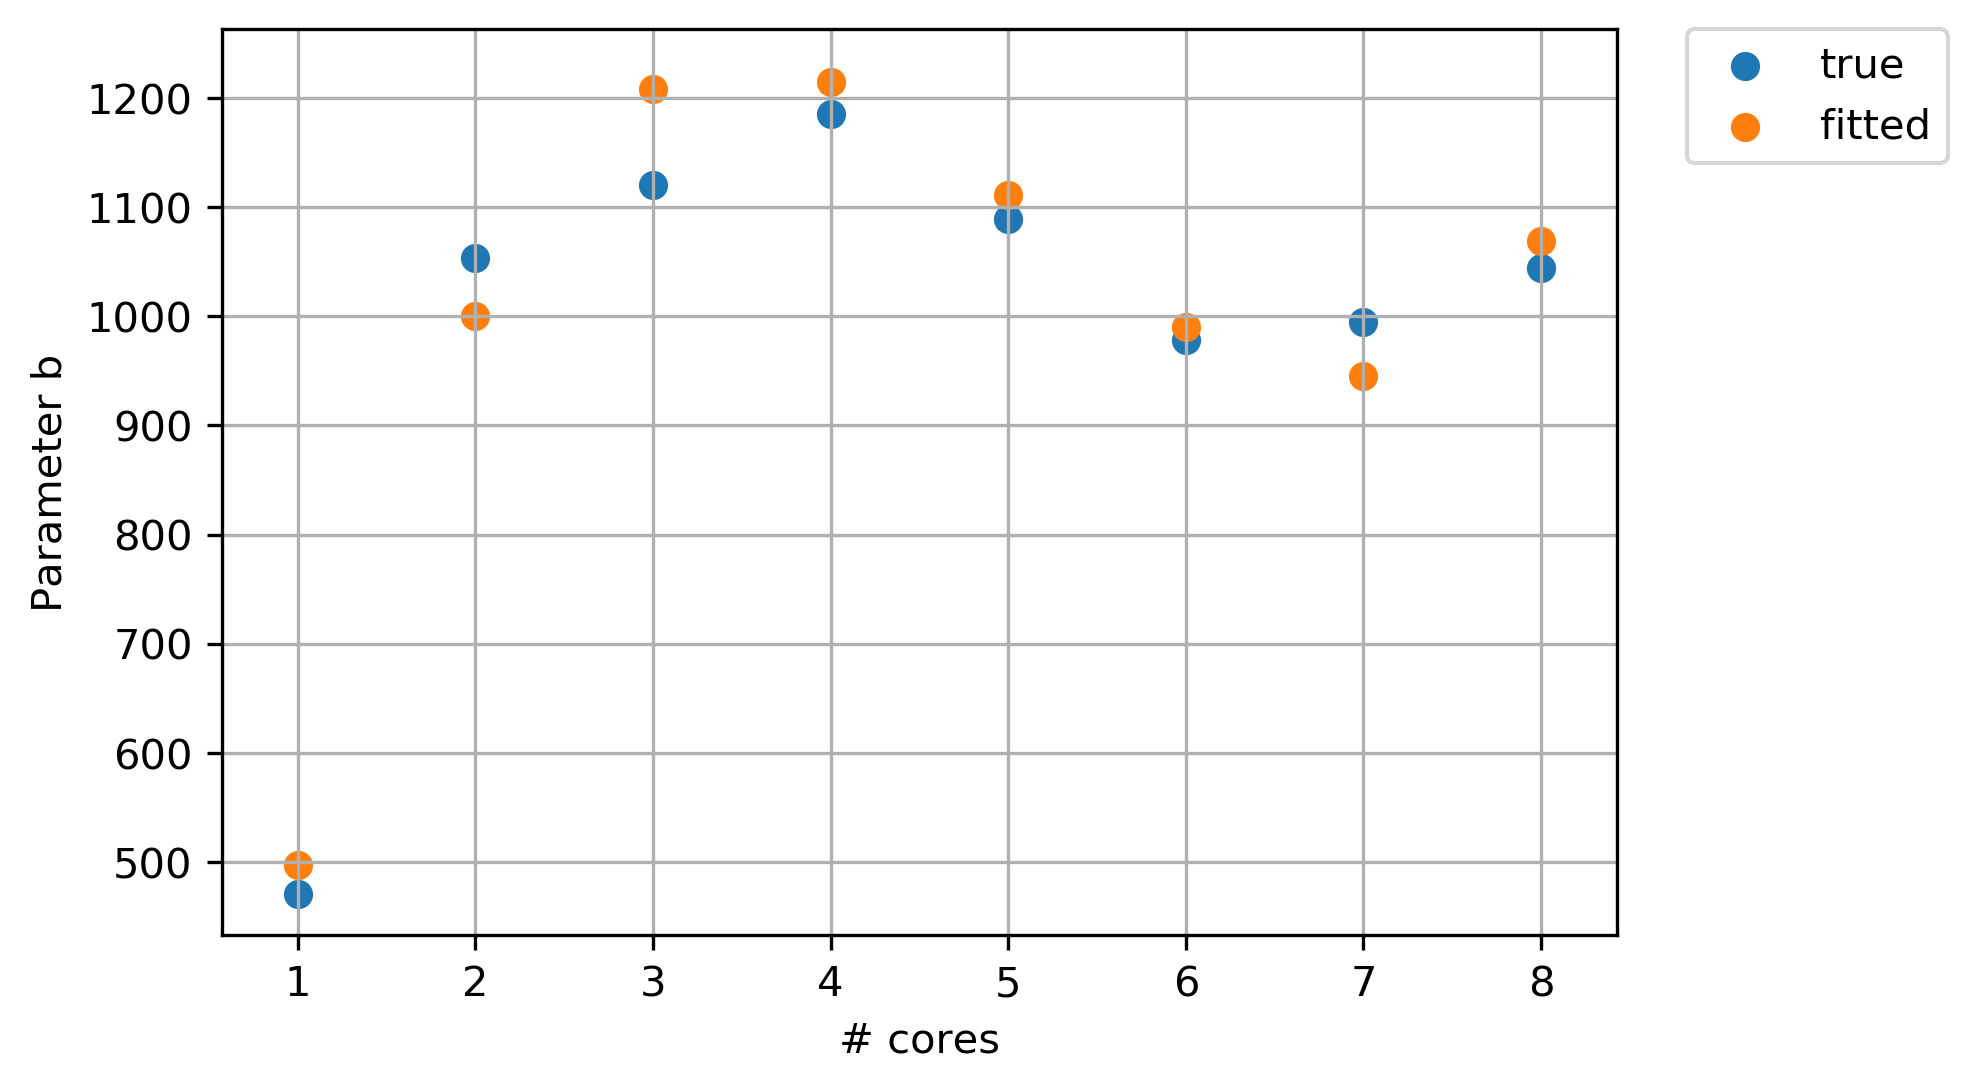
\includegraphics[scale=.2]{images/polyfit/fig_690_params_1.png}\label{fig15:b}}
			{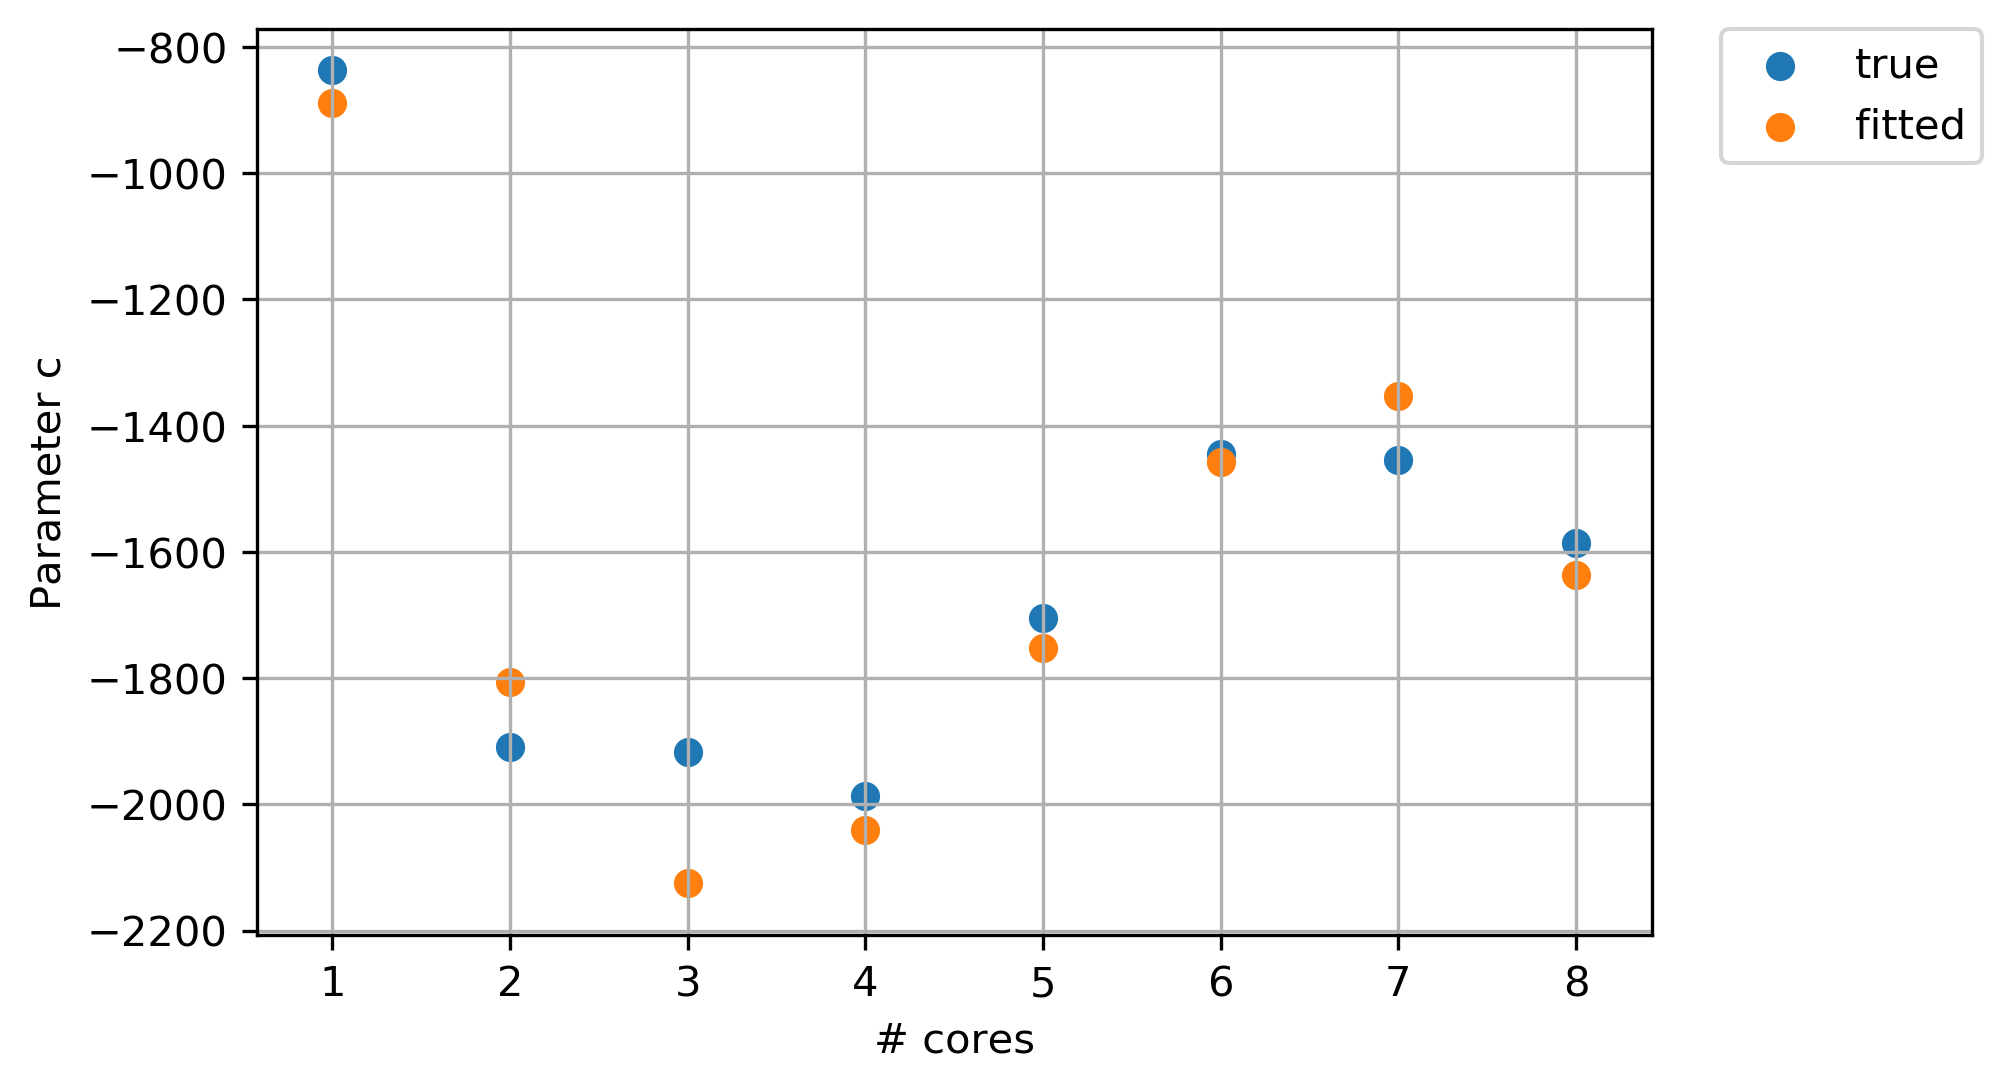
\includegraphics[scale=.2]{images/polyfit/fig_690_params_2.png}\label{fig15:c}}
			\caption{Fitting the parameters of the polynomial function with a $3$rd degree polynomial from the $DMATDMATADD$ benchmark for matrix size $690\times690$ against different number of cores.}	
			\label{fig15}
		\end{figure}
	\end{outline}
\end{frame}


\begin{frame}{Method: Modeling Performance based on Grain Size}
	\begin{outline}
		The final model: $$P=a_{11}g^2N^3+a_{10}g^2N^2+...+a_1N+a_0$$
	\begin{figure}[H]
		\centering
		{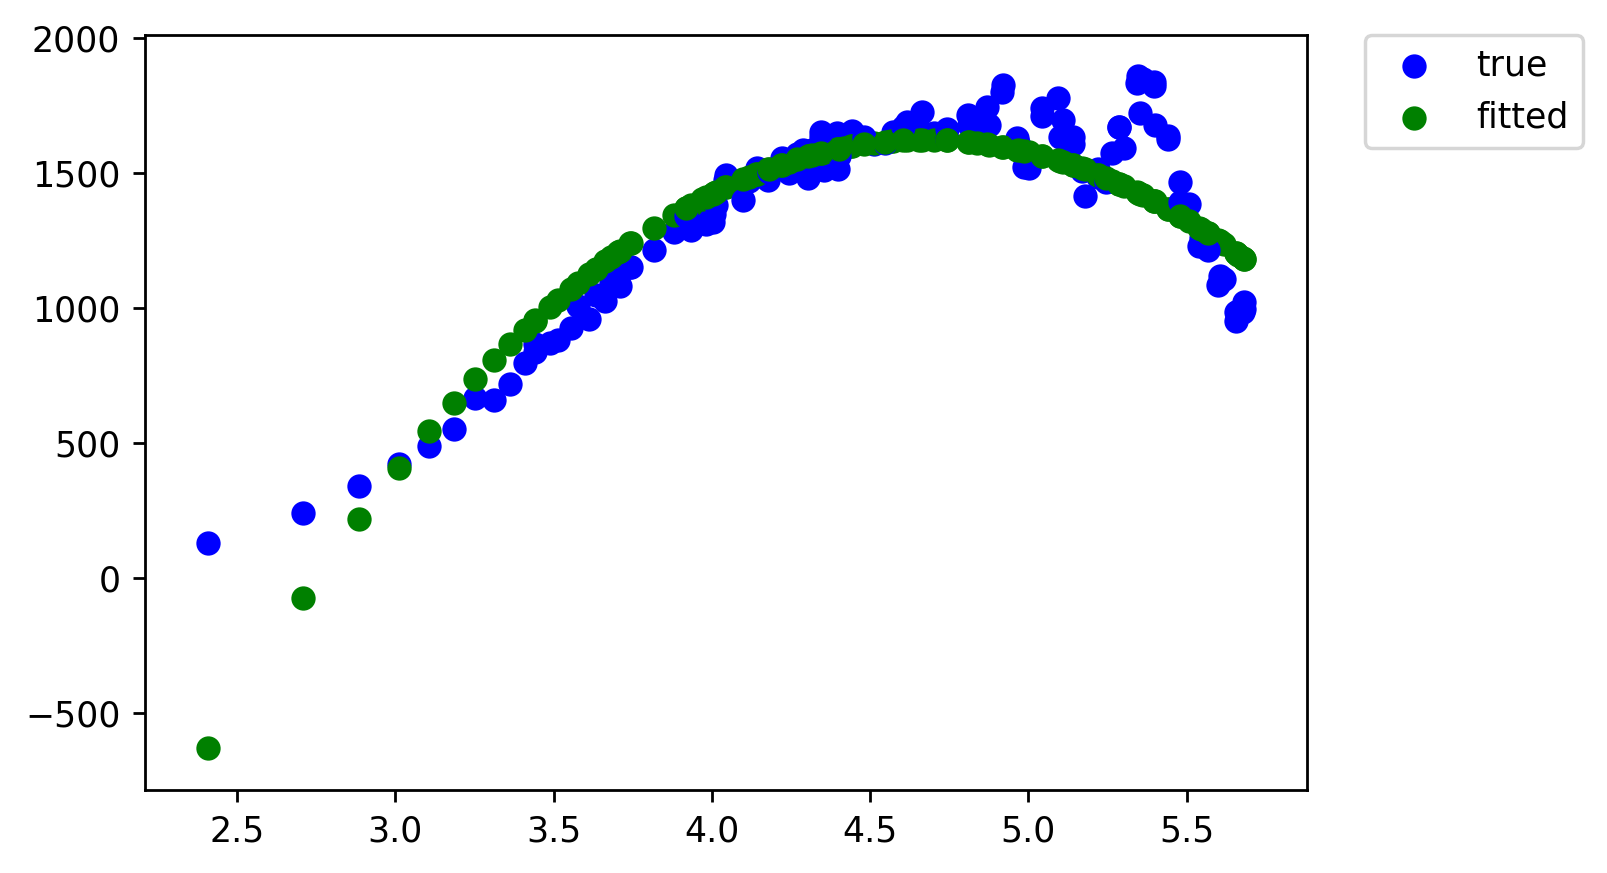
\includegraphics[scale=.3]{images/polyfit/fig_690_total_2.png}\label{fig18:a}}
		{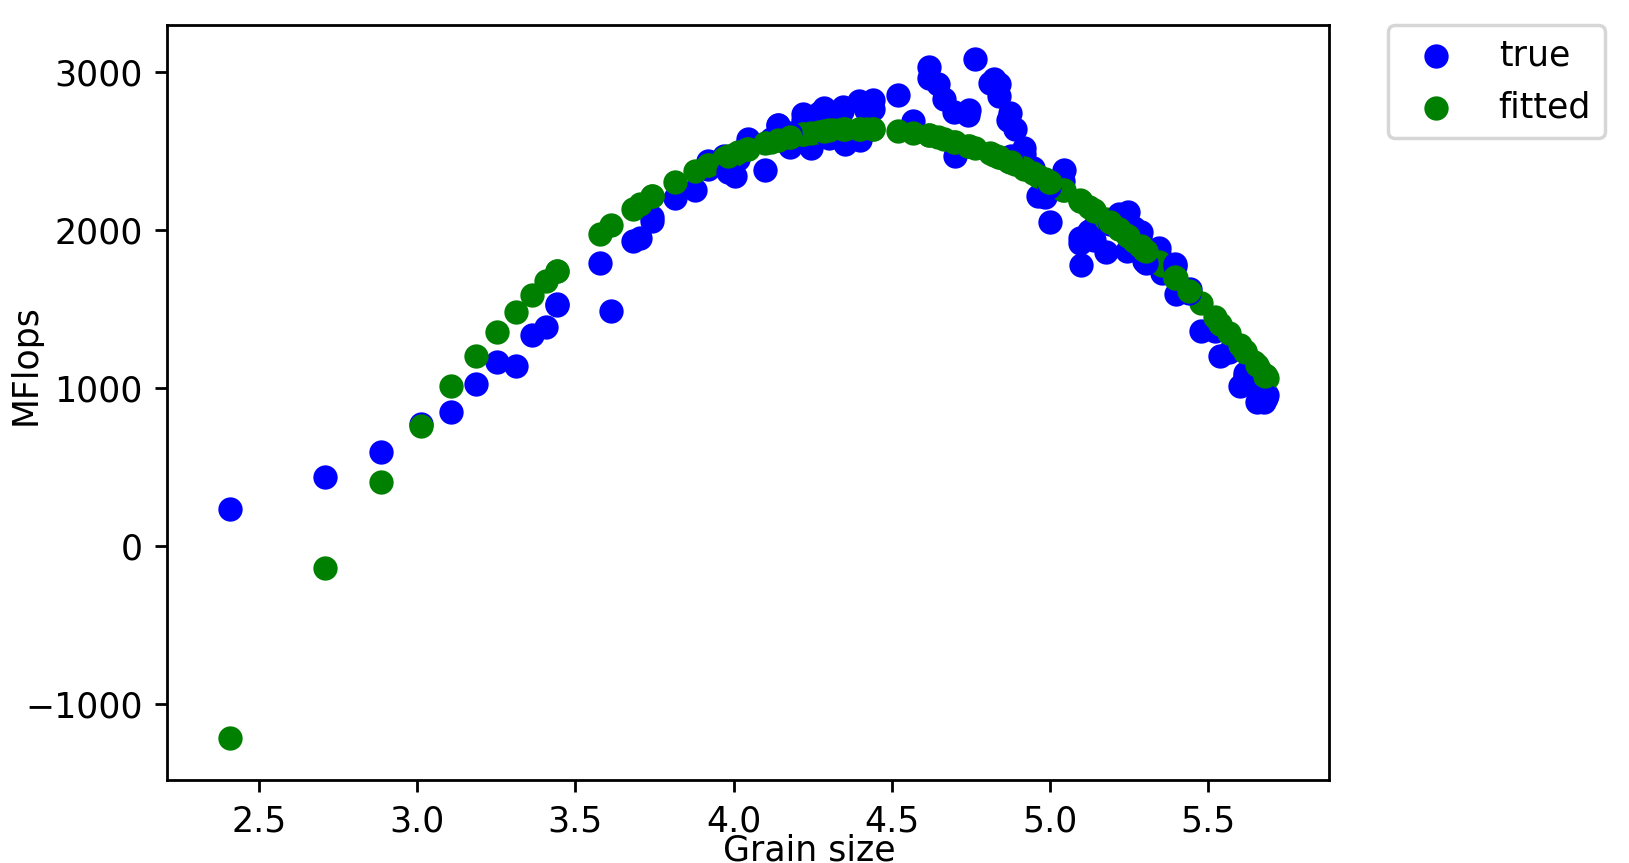
\includegraphics[scale=.3]{images/polyfit/fig_690_total_4.png}\label{fig18:b}}
		{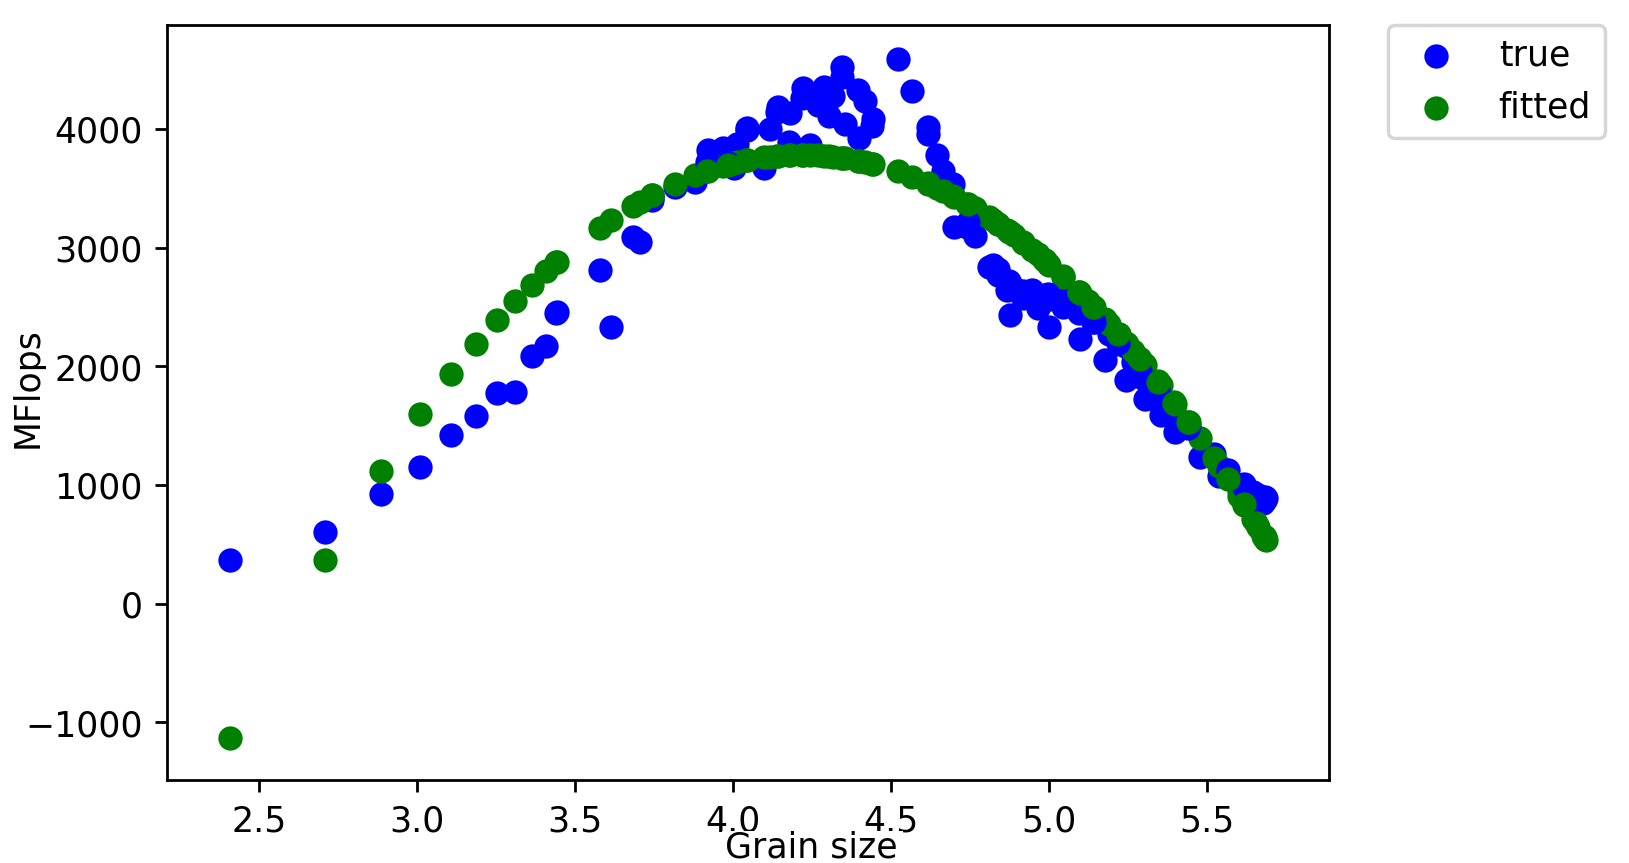
\includegraphics[scale=.3]{images/polyfit/fig_690_total_8.png}\label{fig18:c}}
		\caption{matrix size $690\times690$ for (a) 2 core, (b) 4 cores, (c) 8 cores.}	
		\label{fig18}
	\end{figure}
	\end{outline}
\end{frame}

\begin{frame}{Method: Modeling Performance based on Grain Size}
	\begin{outline}
\begin{figure}[H]
	\centering
	{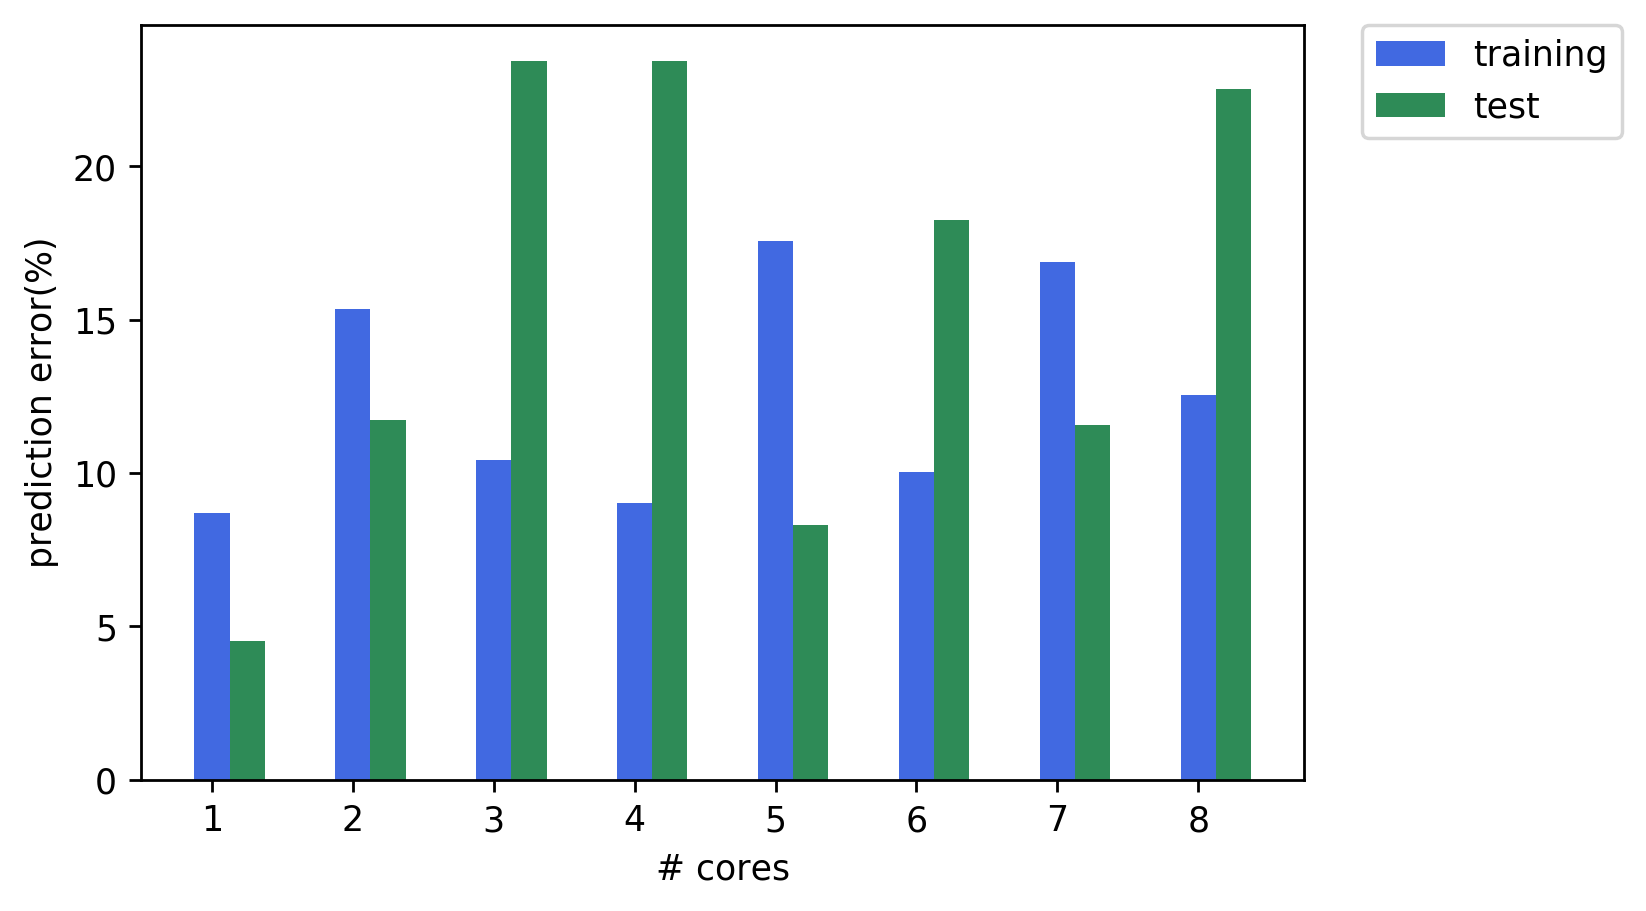
\includegraphics[scale=.35]{images/polyfit/fig_690_total_error.png}\label{fig17:a}}
	{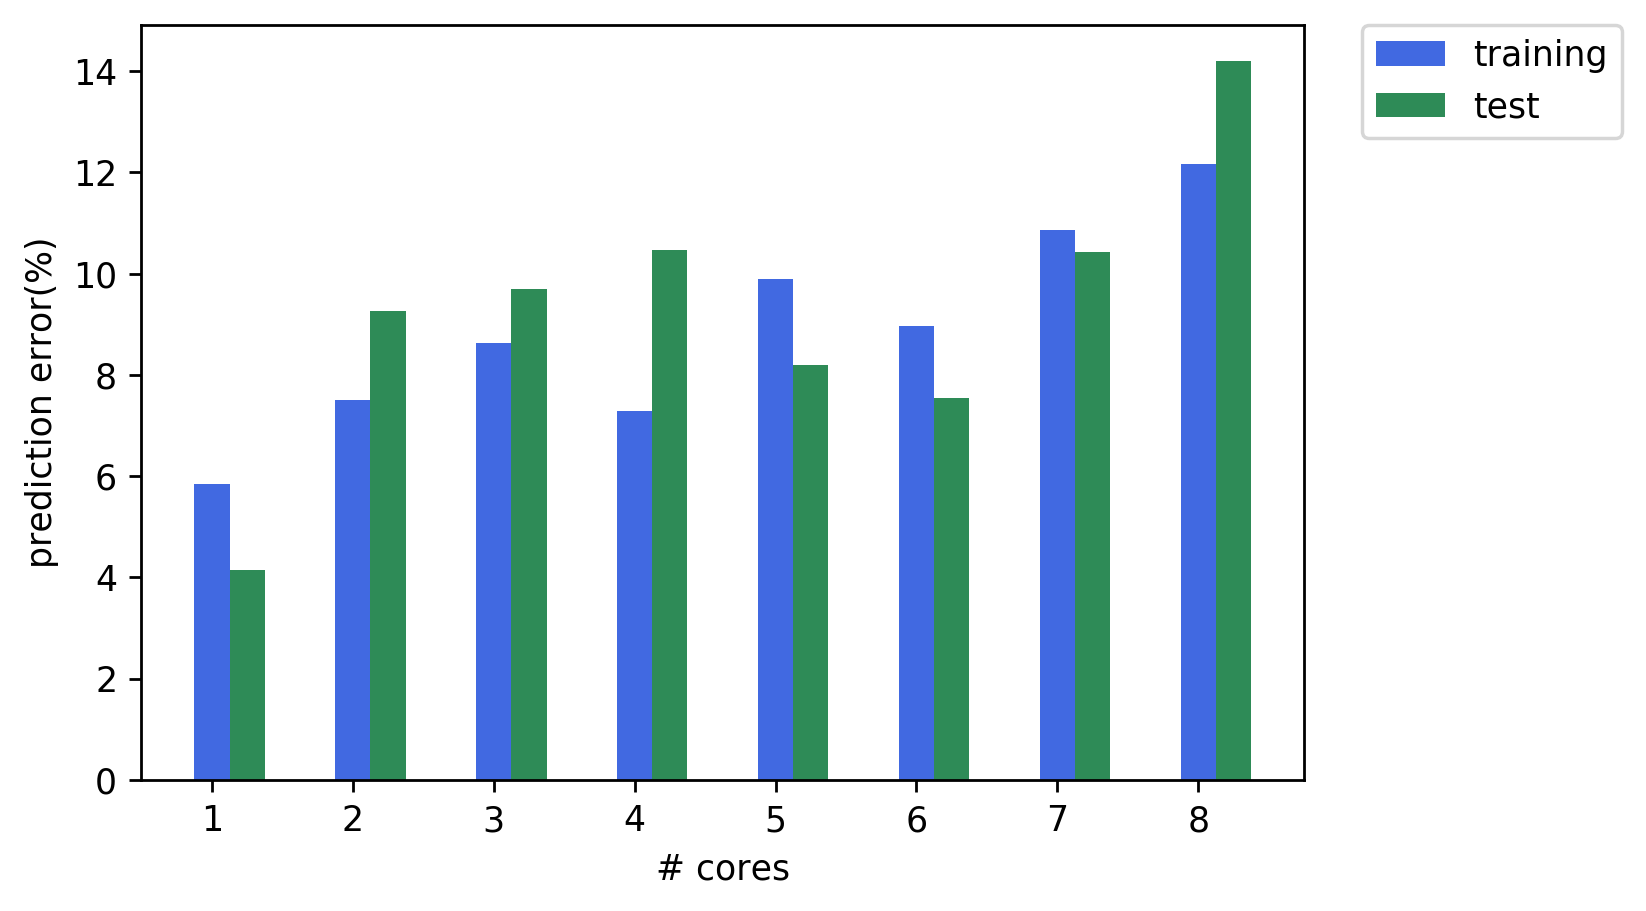
\includegraphics[scale=.35]{images/polyfit/fig_690_total_error_corrected.png}\label{fig17:b}}
	\caption{(a) All the data points are include in calculation of error, (b) the leftmost sample was removed from error calculation.}	
	\label{fig17}
\end{figure}
	\end{outline}
\end{frame}

\begin{frame}{Method: Finding the Grain Size Range for Maximum Performance}
	\begin{outline}
\begin{figure}[H]
	\centering
	{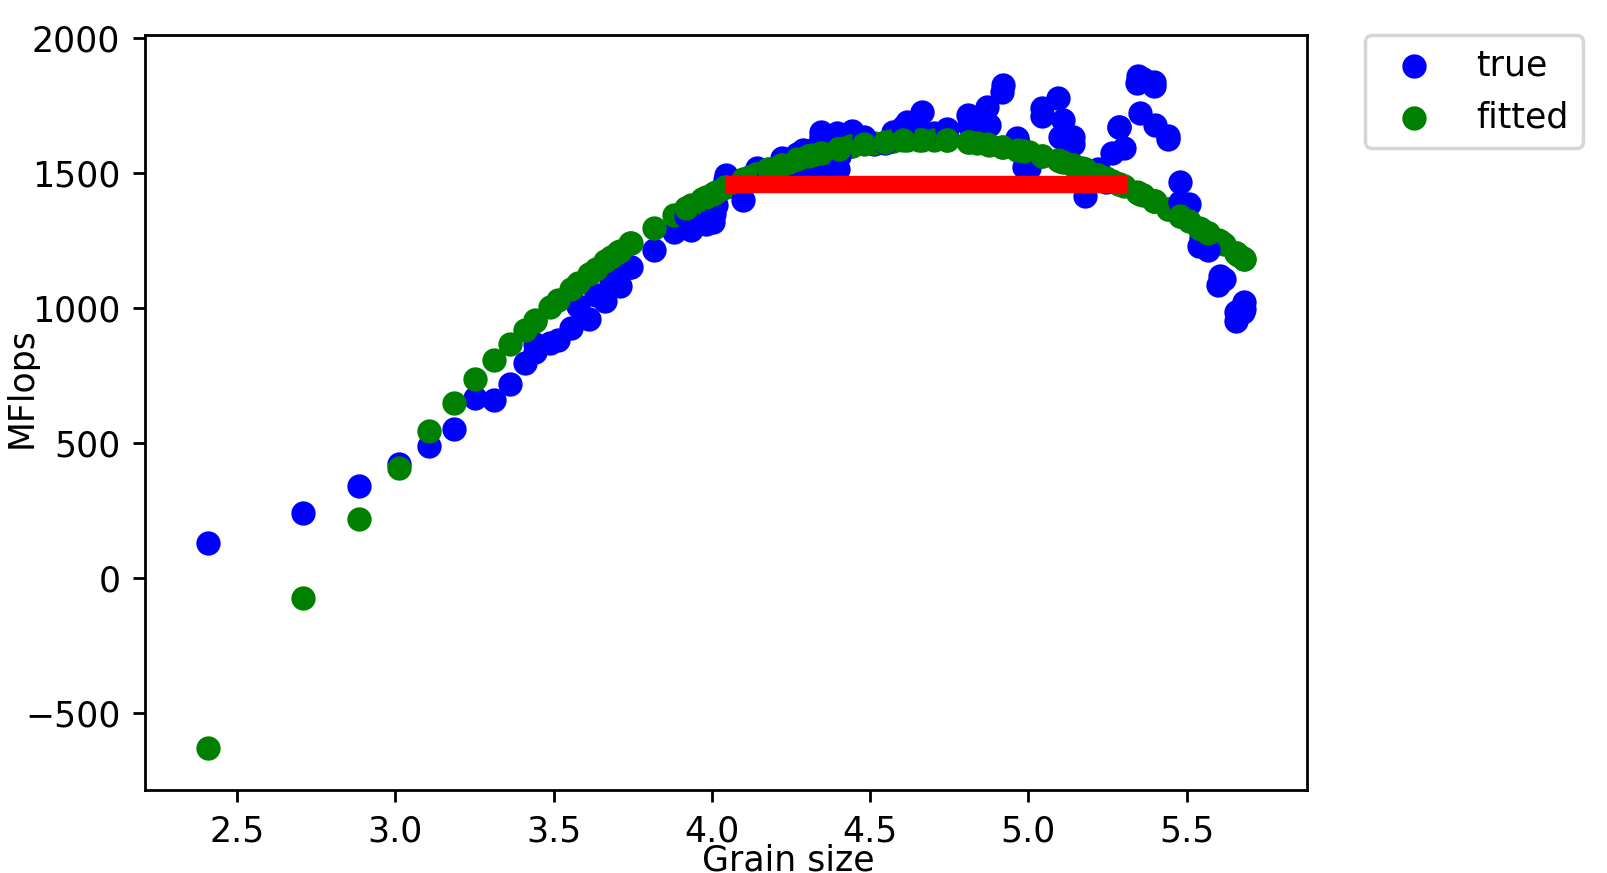
\includegraphics[scale=.3]{images/polyfit/fig_690_total_2_range.png}\label{fig12:a}}
	{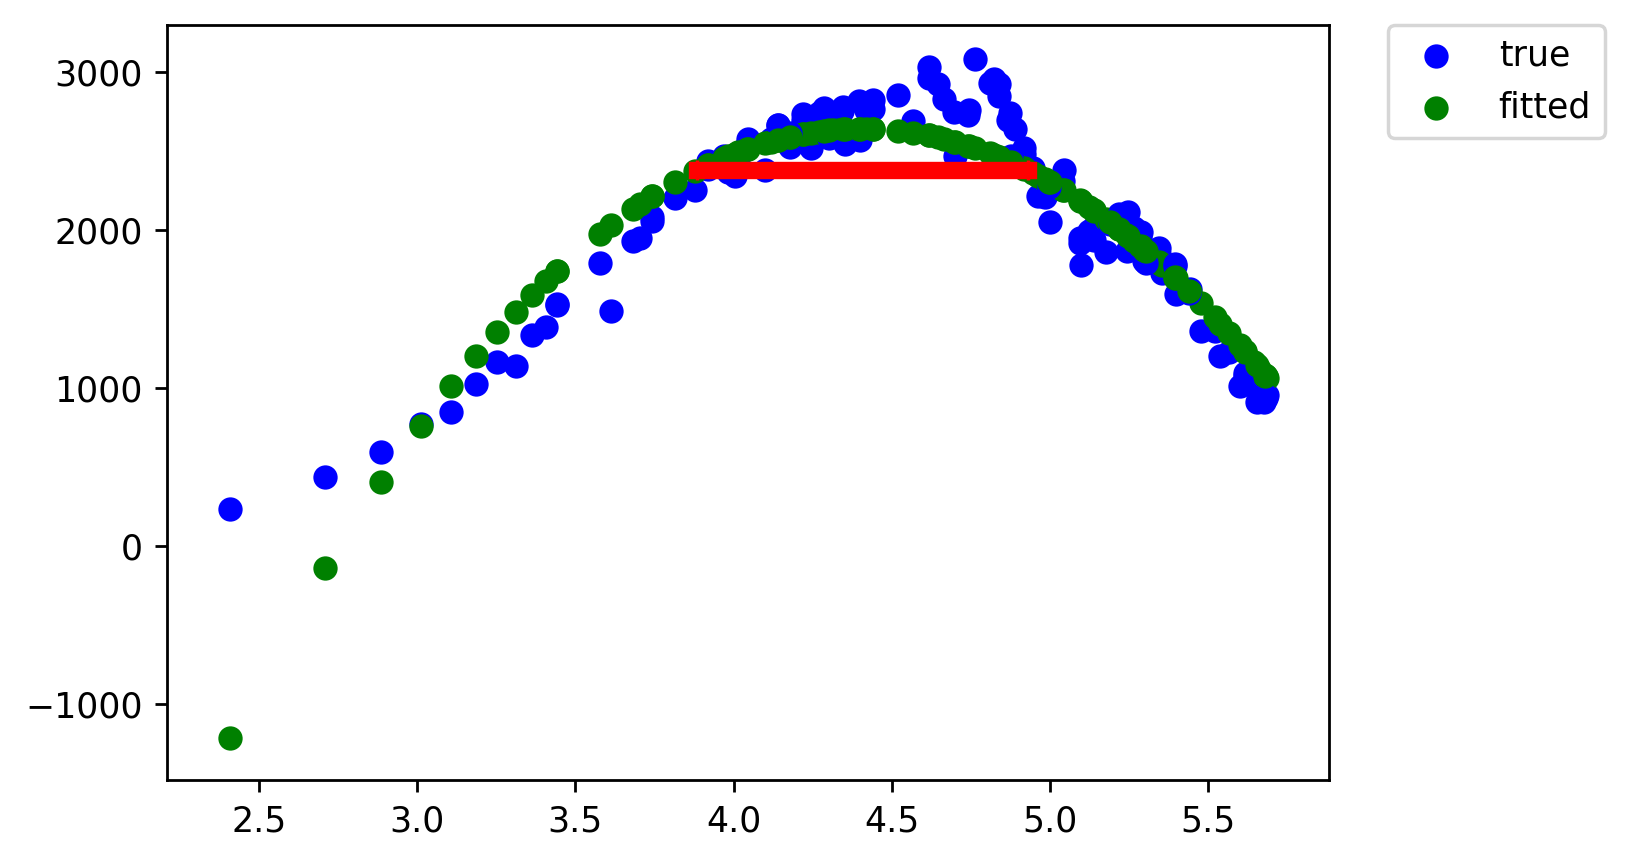
\includegraphics[scale=.3]{images/polyfit/fig_690_total_4_range.png}\label{fig12:b}}
	{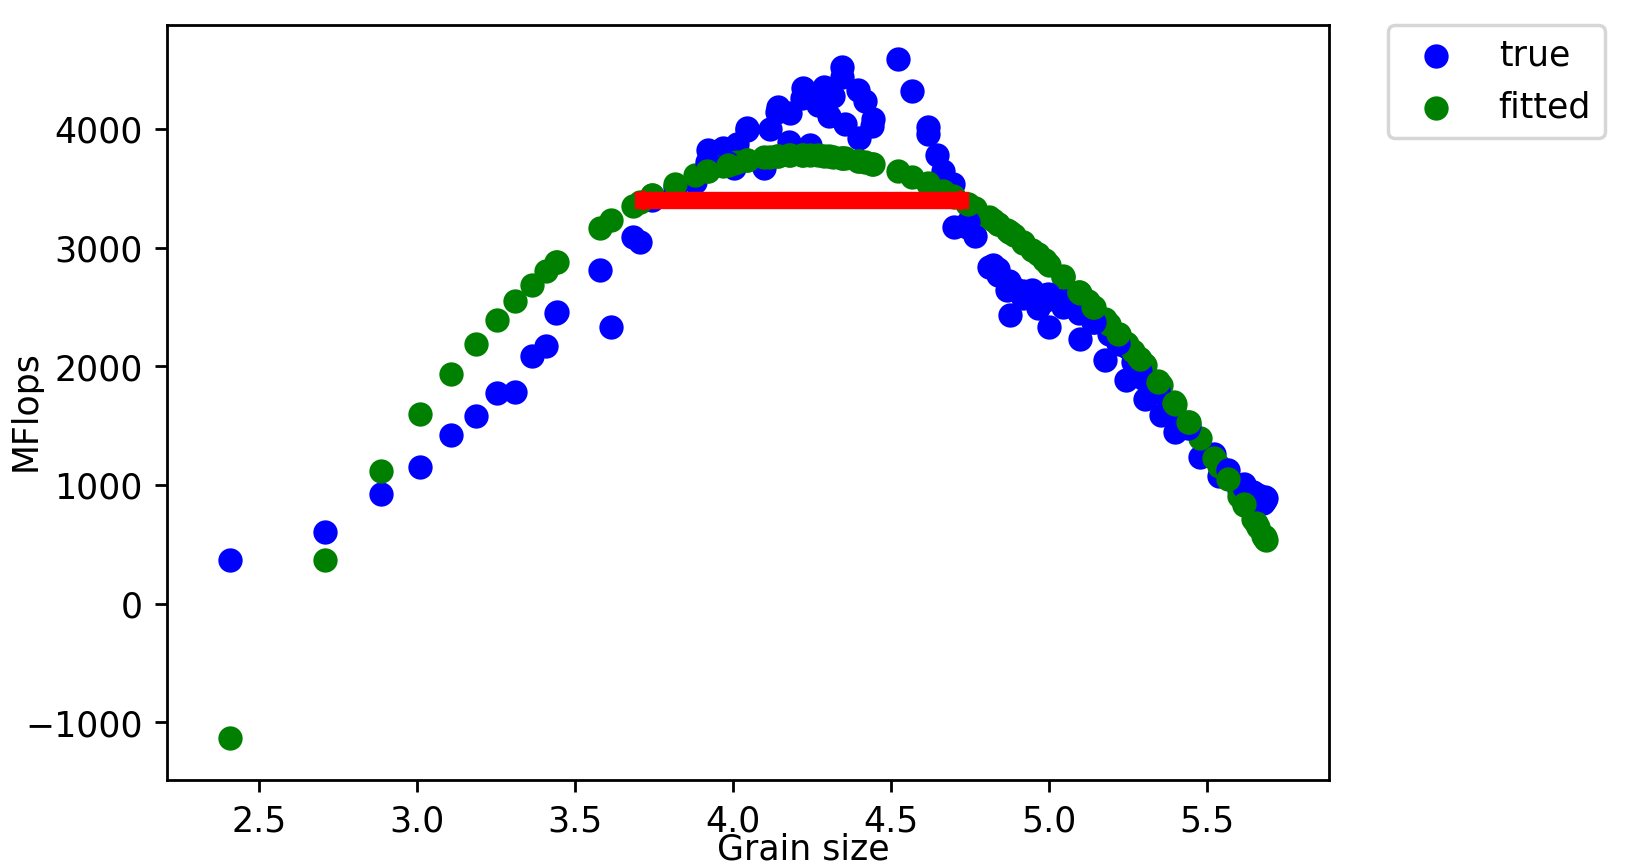
\includegraphics[scale=.3]{images/polyfit/fig_690_total_8_range.png}\label{fig12:c}}
	\caption{The range of grain size (shown as the red line) that leads to a performance within $10\%$ of the maximum performance for (a) 2 cores, (b) 4 cores and (b) 8 cores.}	
	\label{fig12}
\end{figure}
	\end{outline}
\end{frame}

\begin{frame}{Method: Finding the Grain Size Range for Maximum Performance}
	\begin{outline}
		\begin{figure}[H]
			\centering
			{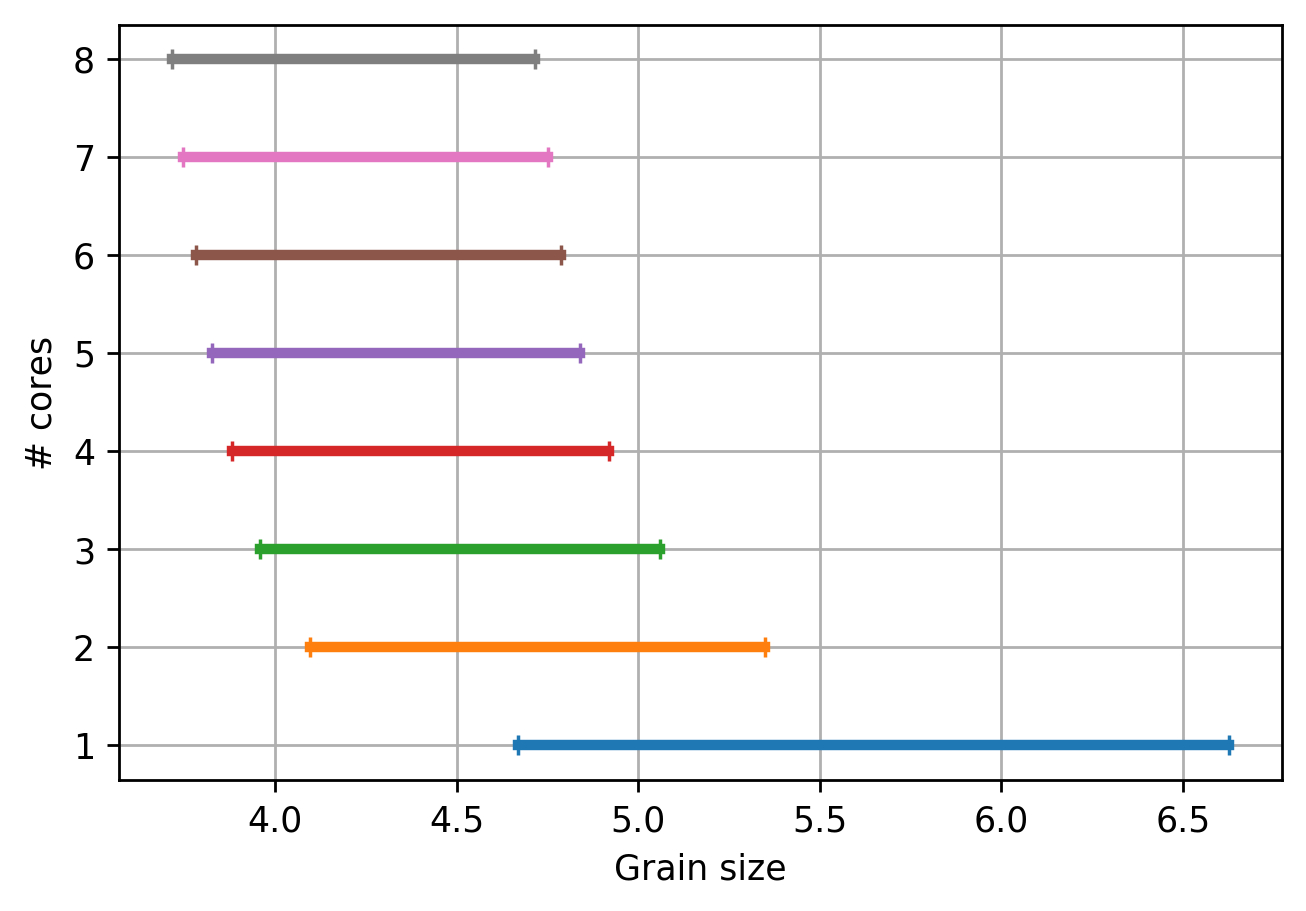
\includegraphics[scale=.3]{images/polyfit/fig_690_peak_range_all.png}\label{fig13:a}}
%			{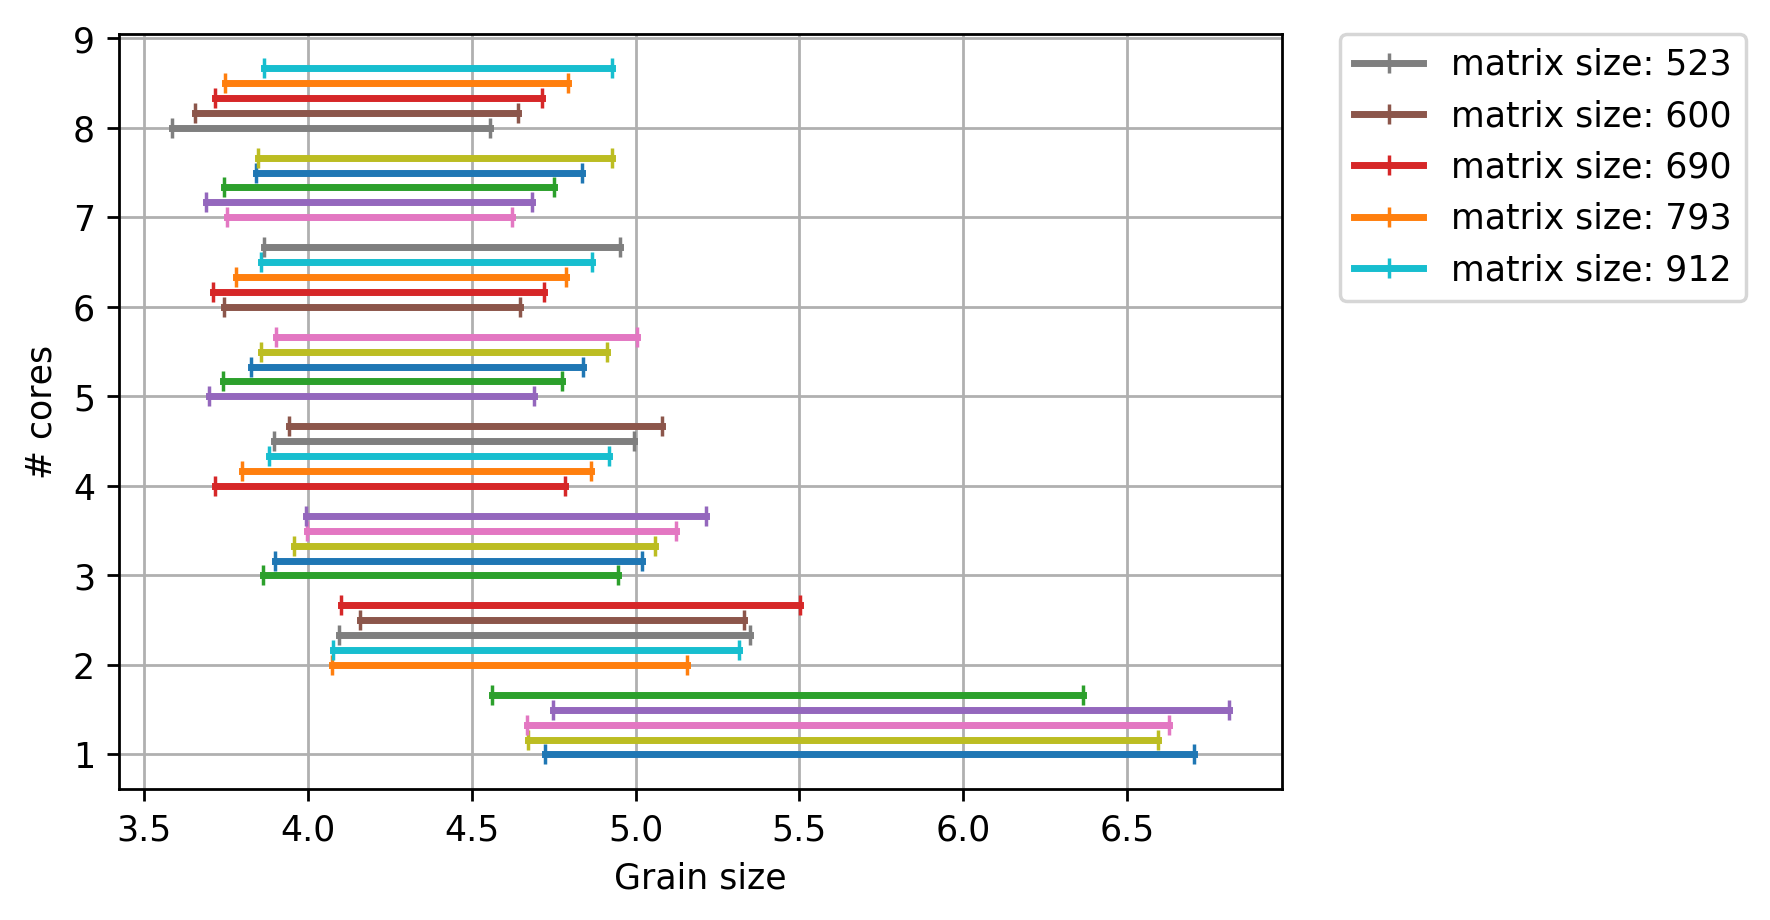
\includegraphics[scale=.3]{images/polyfit/fig_523-912_peak_range_all.png}\label{fig13:b}}
			\caption{The range of grain size within $10\%$ of the maximum performance of the fitted polynomial function for $DMATDMATADD$ benchmark for different number of cores for (a) matrix size $690\times690$}	
			\label{fig13}
\end{figure}
\end{outline}
\end{frame}


\begin{frame}{Method: Finding the Grain Size Range for Maximum Performance}
	\begin{outline}
\begin{figure}[H]
	\centering
	{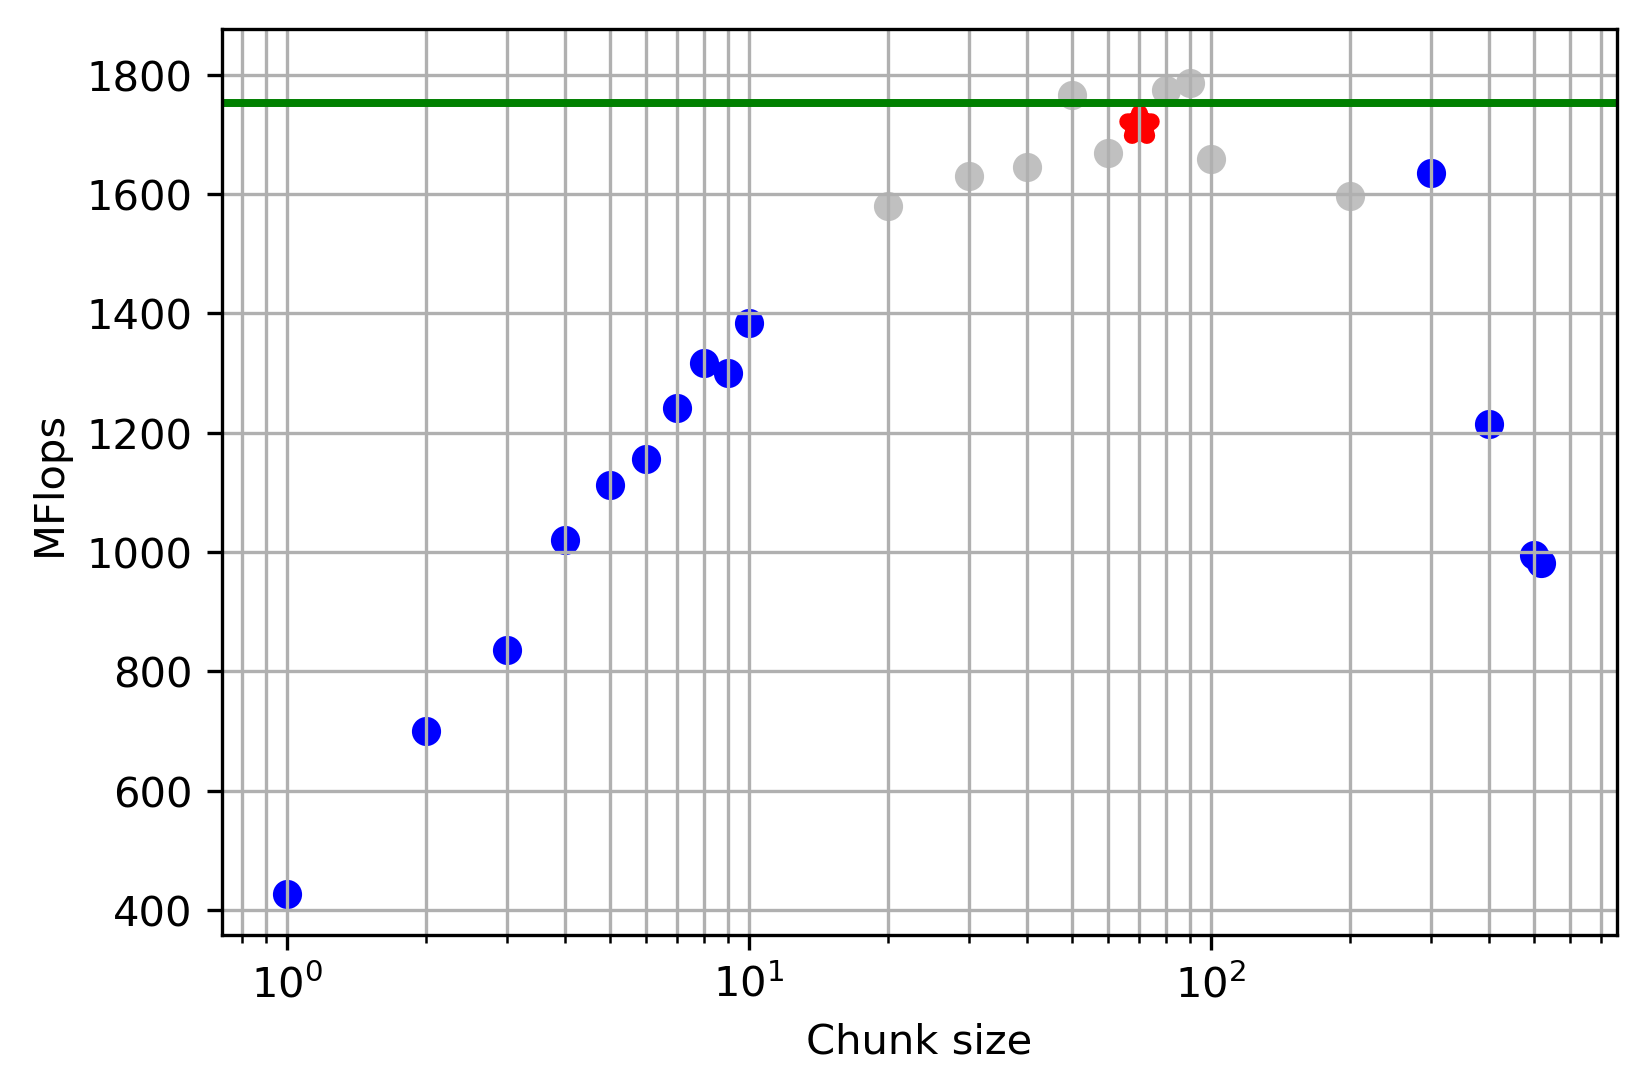
\includegraphics[scale=.25]{images/polyfit/fig_690_chunks_2_4-256.png}\label{fig14:a}}
	{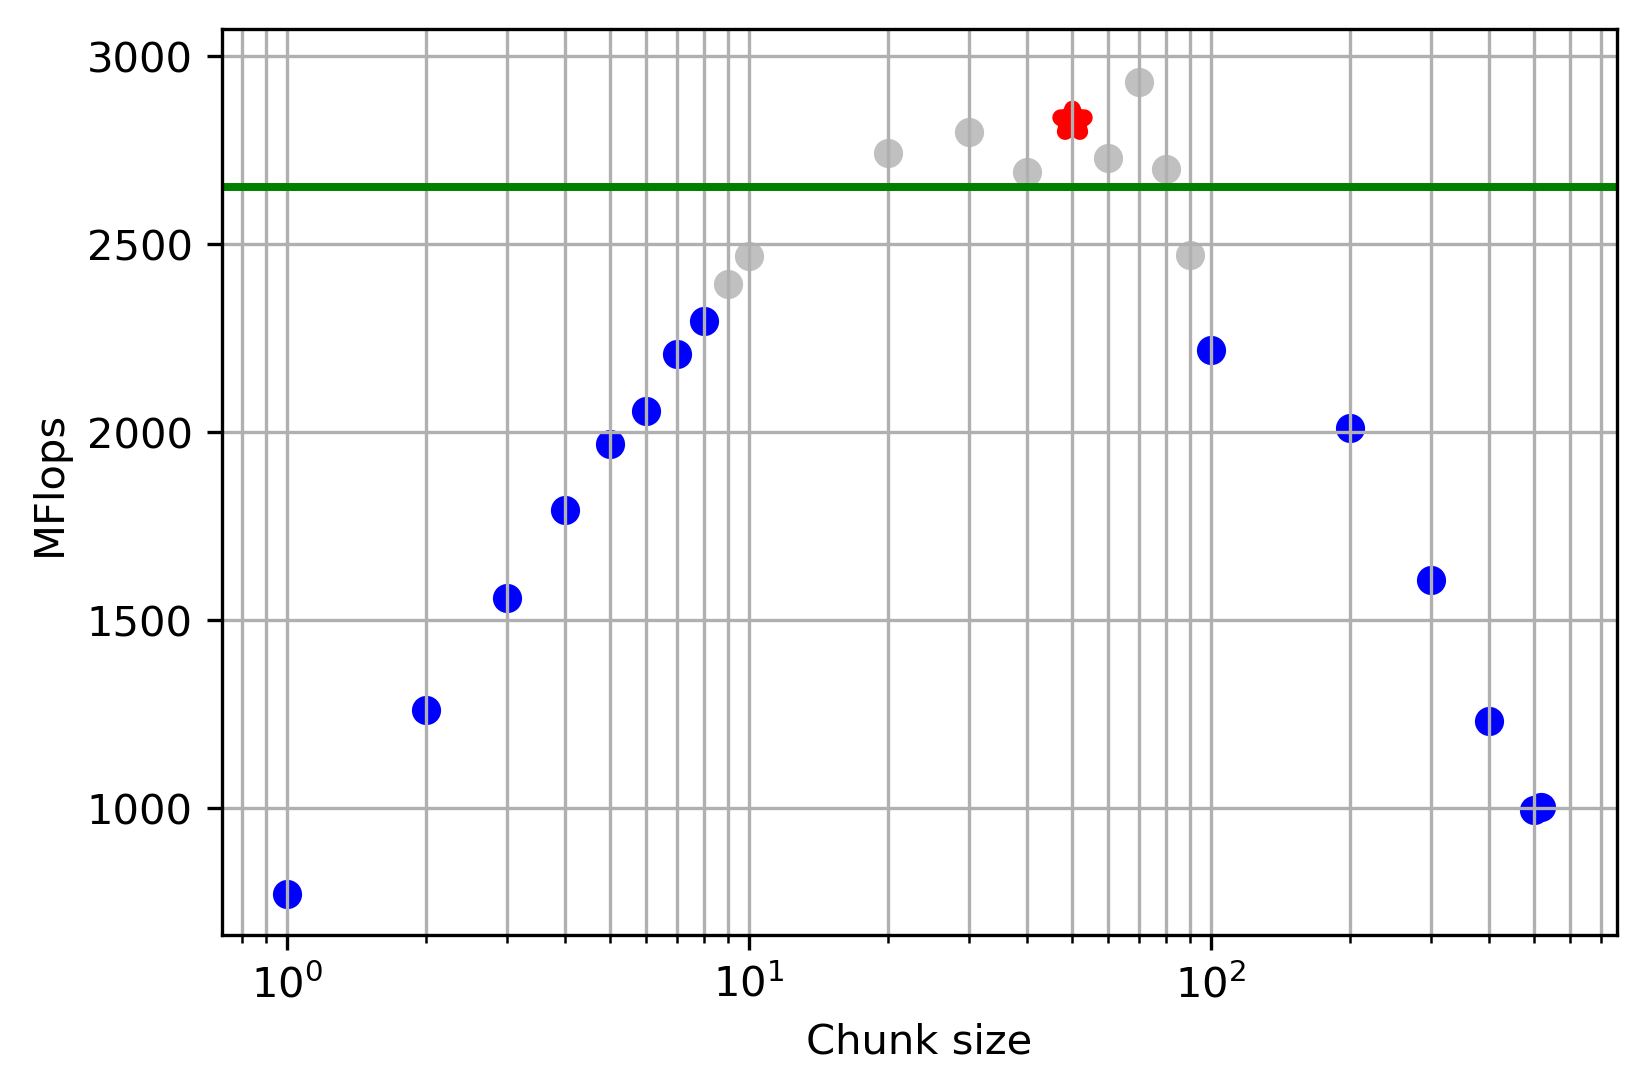
\includegraphics[scale=.25]{images/polyfit/fig_690_chunks_4_4-256.png}\label{fig14:b}}
	{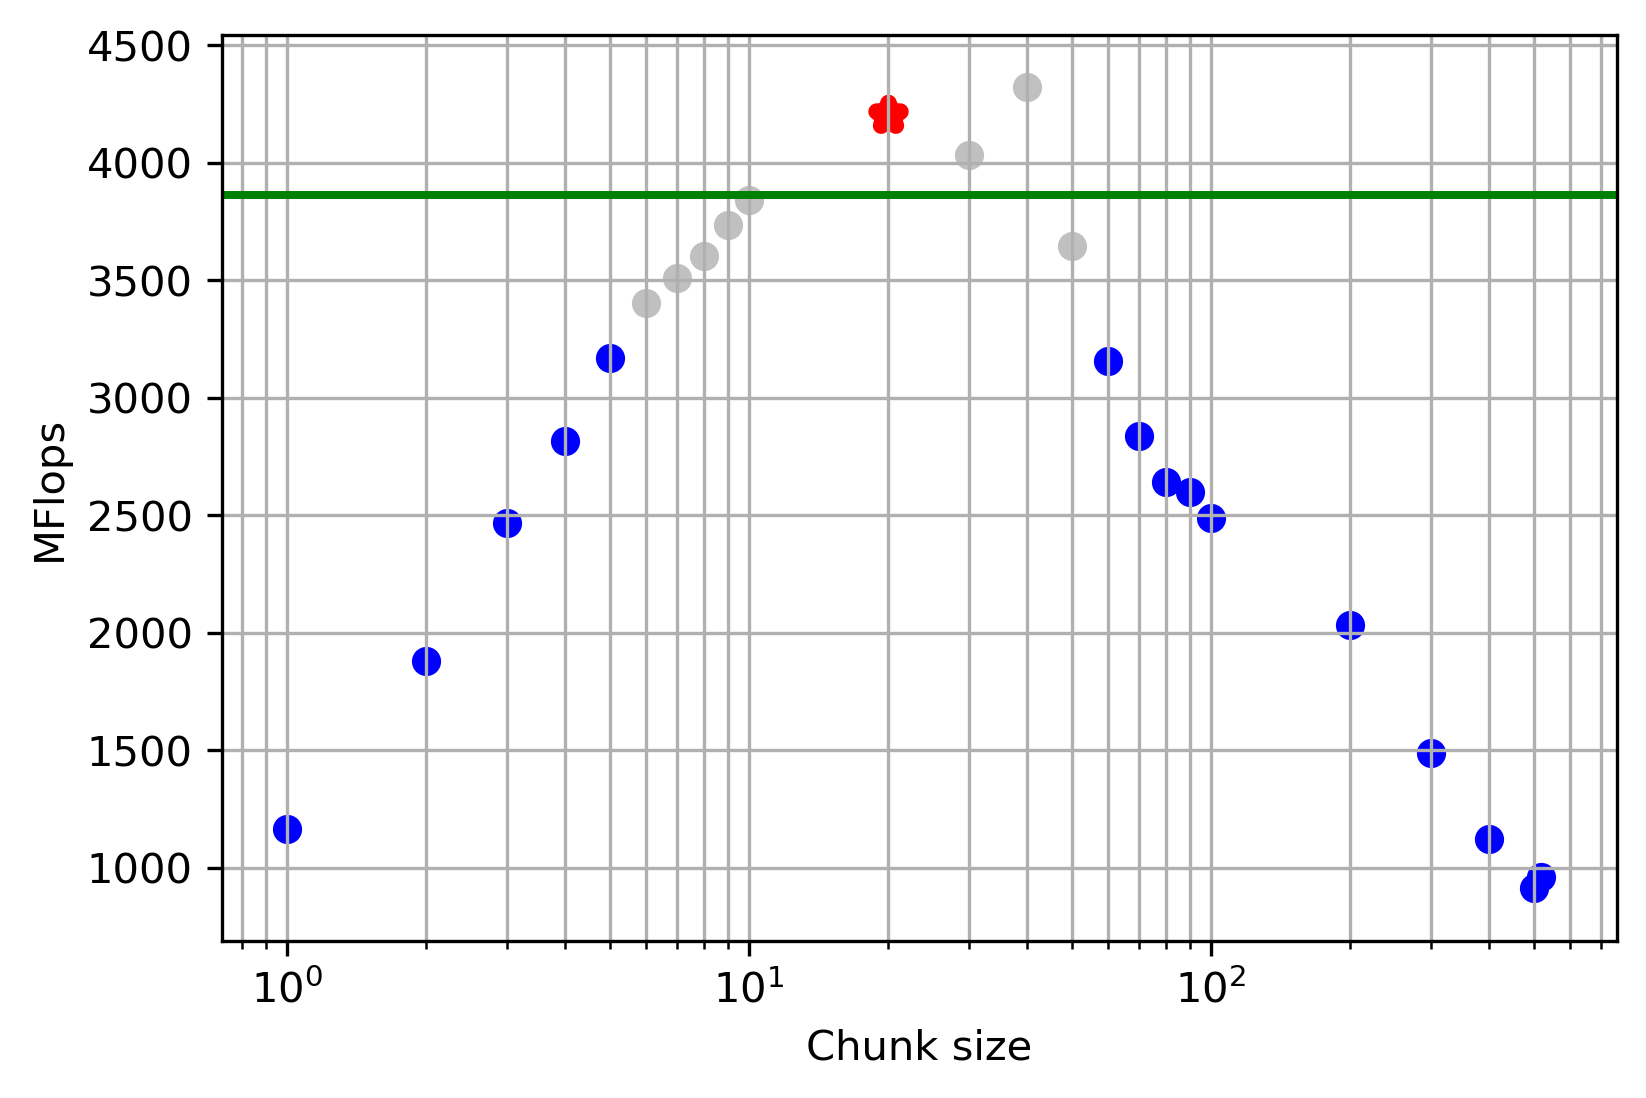
\includegraphics[scale=.25]{images/polyfit/fig_690_chunks_8_4-256.png}\label{fig14:c}}
	{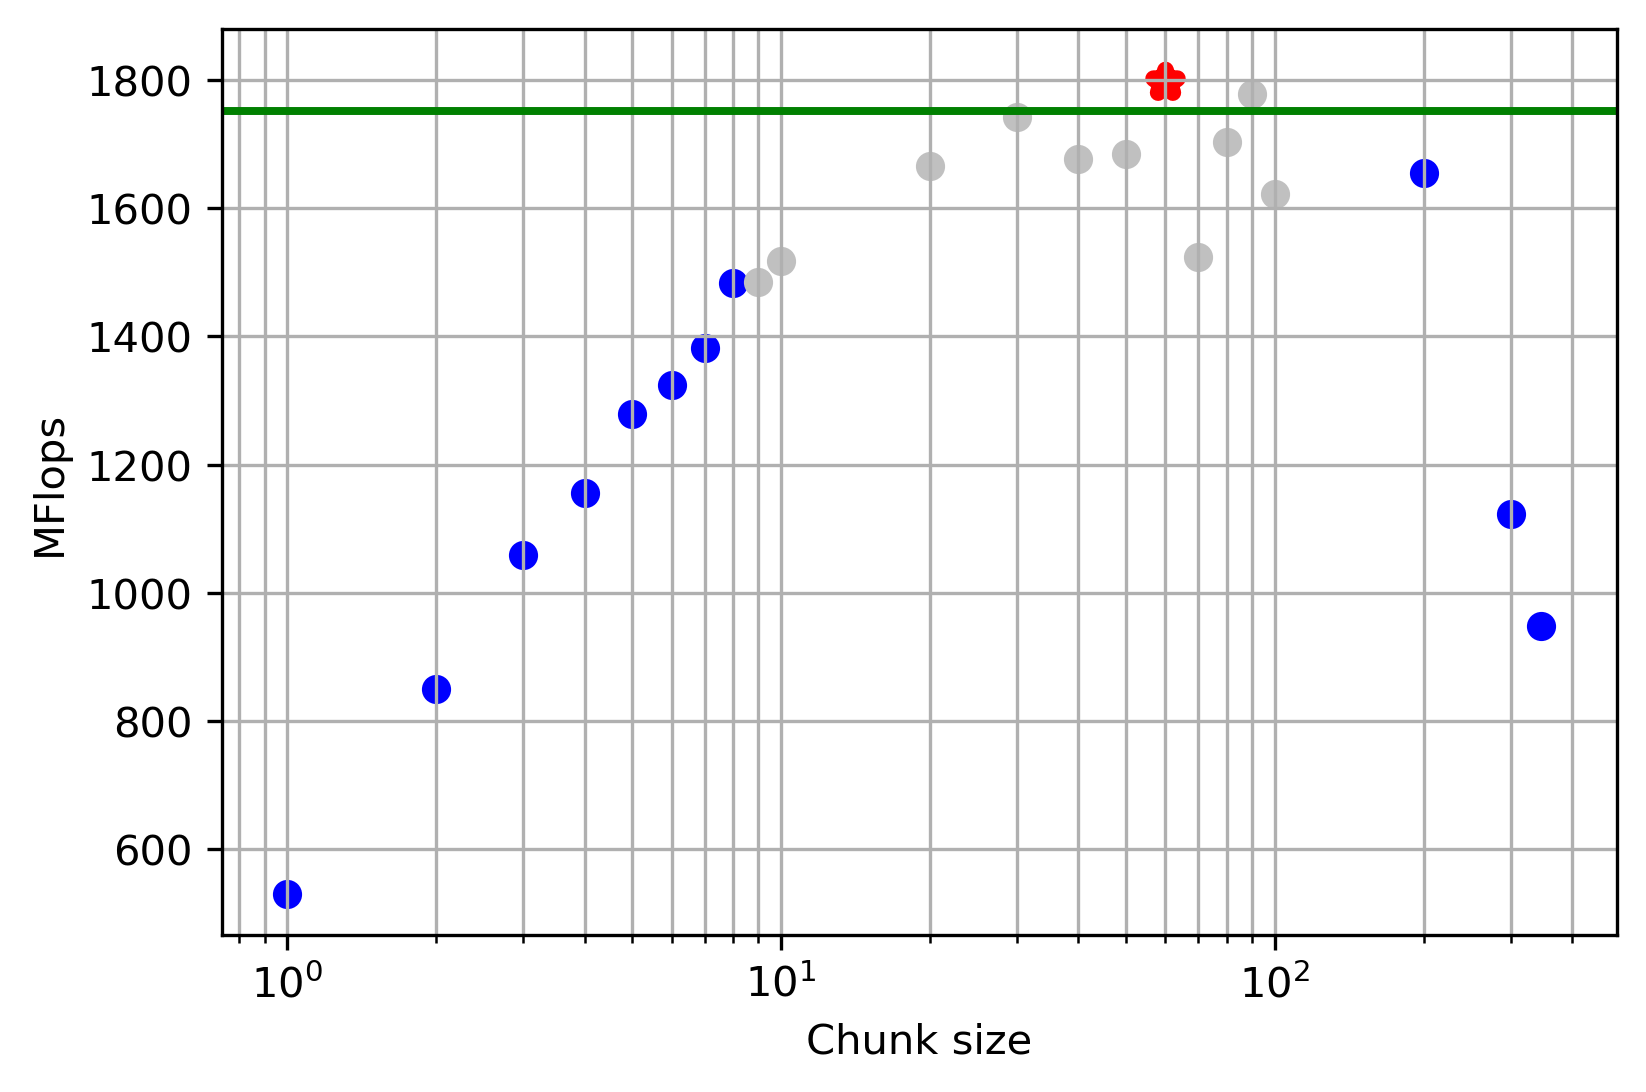
\includegraphics[scale=.25]{images/polyfit/fig_690_chunks_2_4-512.png}\label{fig14:d}}
	{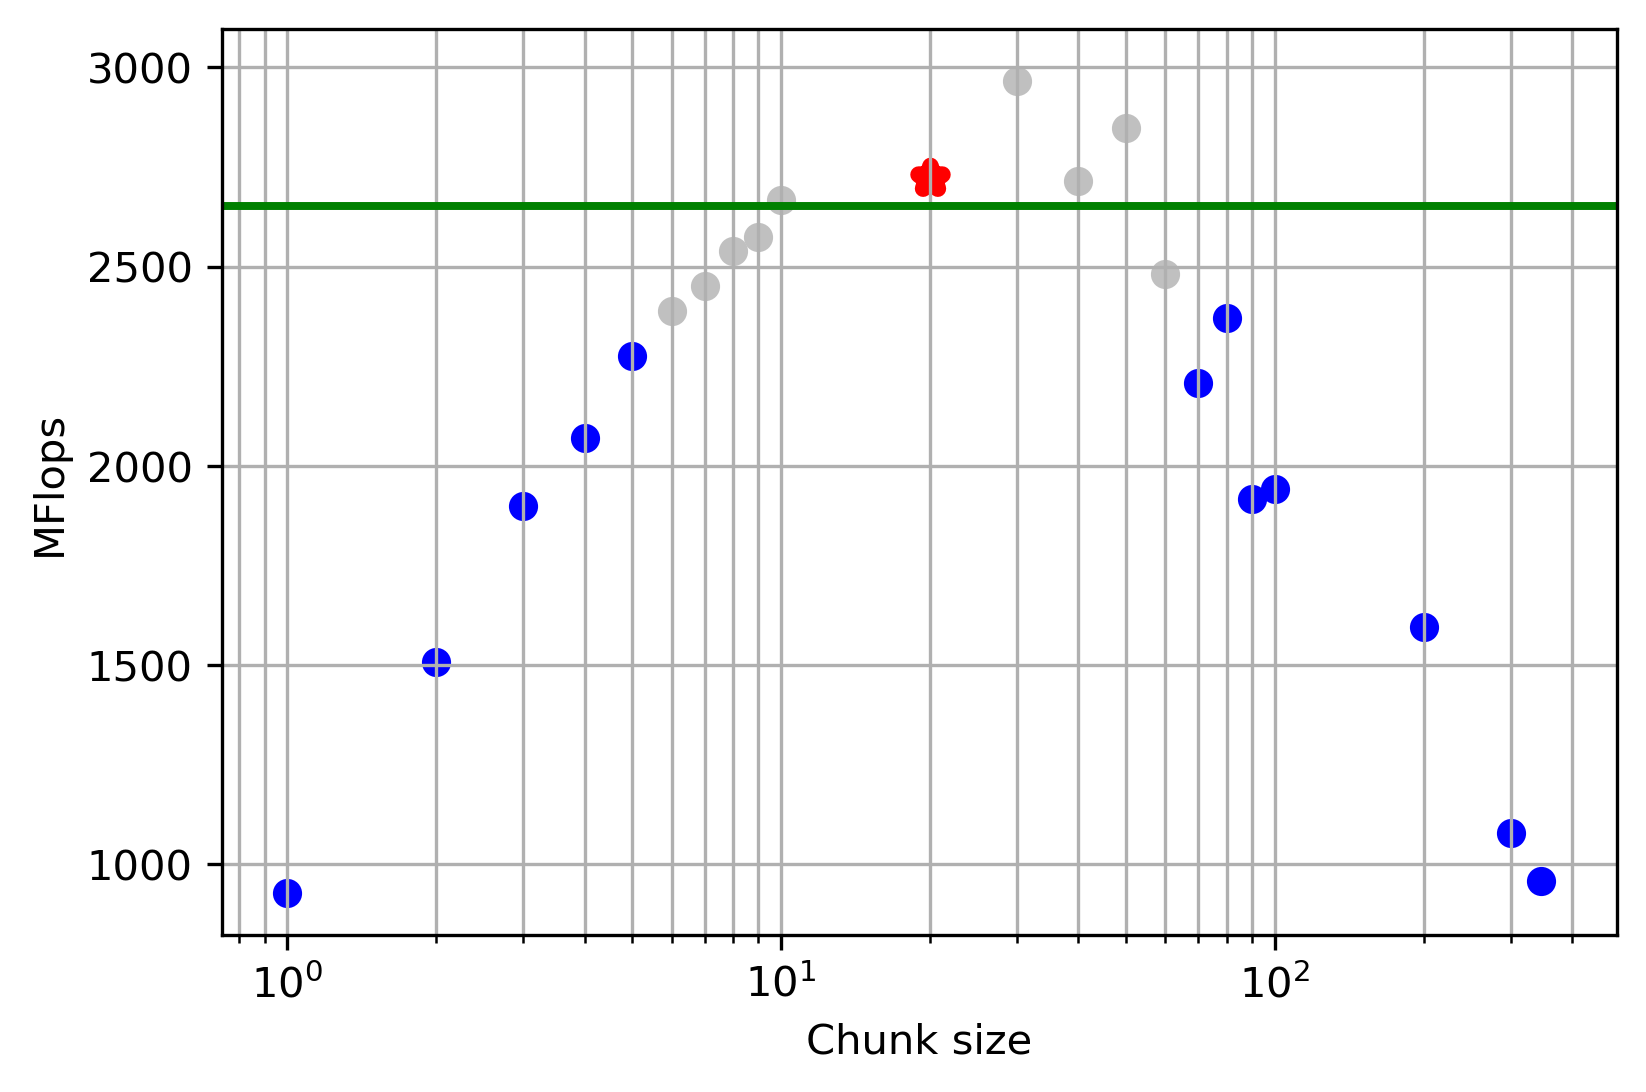
\includegraphics[scale=.25]{images/polyfit/fig_690_chunks_4_4-512.png}\label{fig14:e}}
	{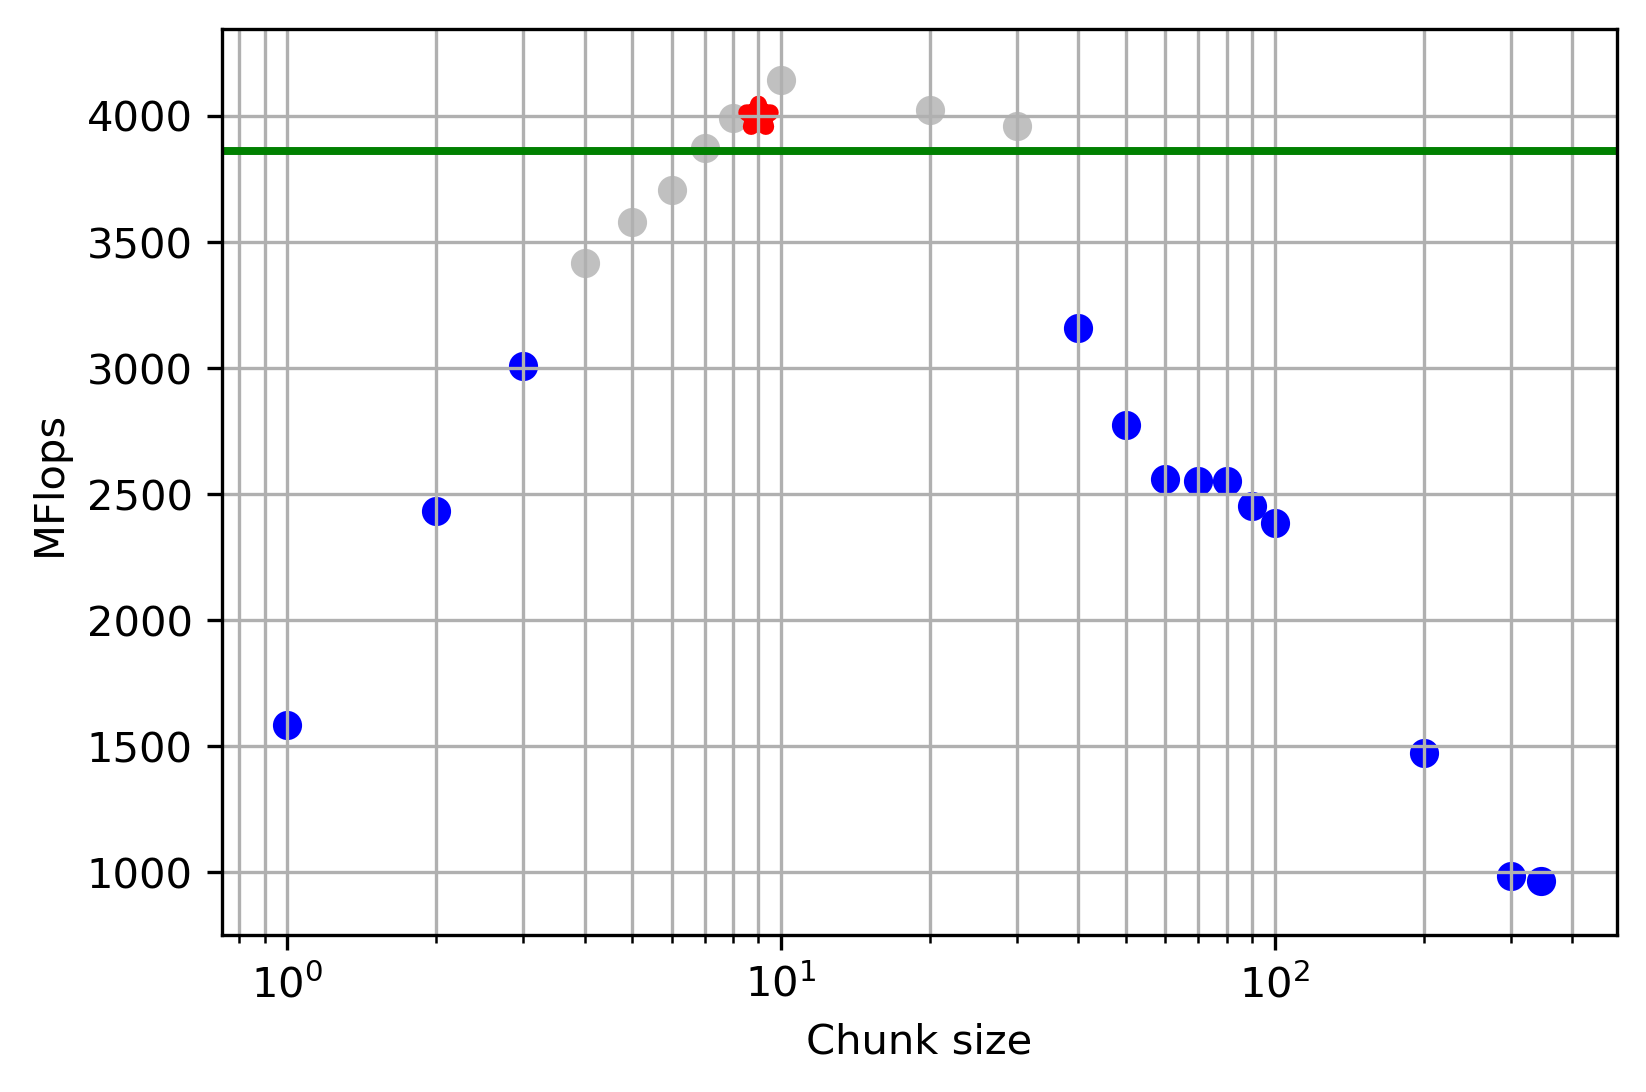
\includegraphics[scale=.25]{images/polyfit/fig_690_chunks_8_4-512.png}\label{fig14:f}}
	\caption{matrix size $690\times690$ with block size of $4\times256$ on (a) $2$ cores, (b) $4$ cores, and (c) $8$ cores, and block size of $4\times512$ on (d) $2$ cores, (e) $4$ cores, and (f) $8$ cores. }	
	\label{fig14}
\end{figure}
\end{outline}
\end{frame}

\begin{frame}{Method: Bathtub Model}
	\begin{outline}
		Creating a analytic model for execution time based on grain size
	\end{outline}
\end{frame}


\begin{frame}{Method: Bathtub Model}
	\begin{outline}
\begin{figure}[H]
	\centering
	{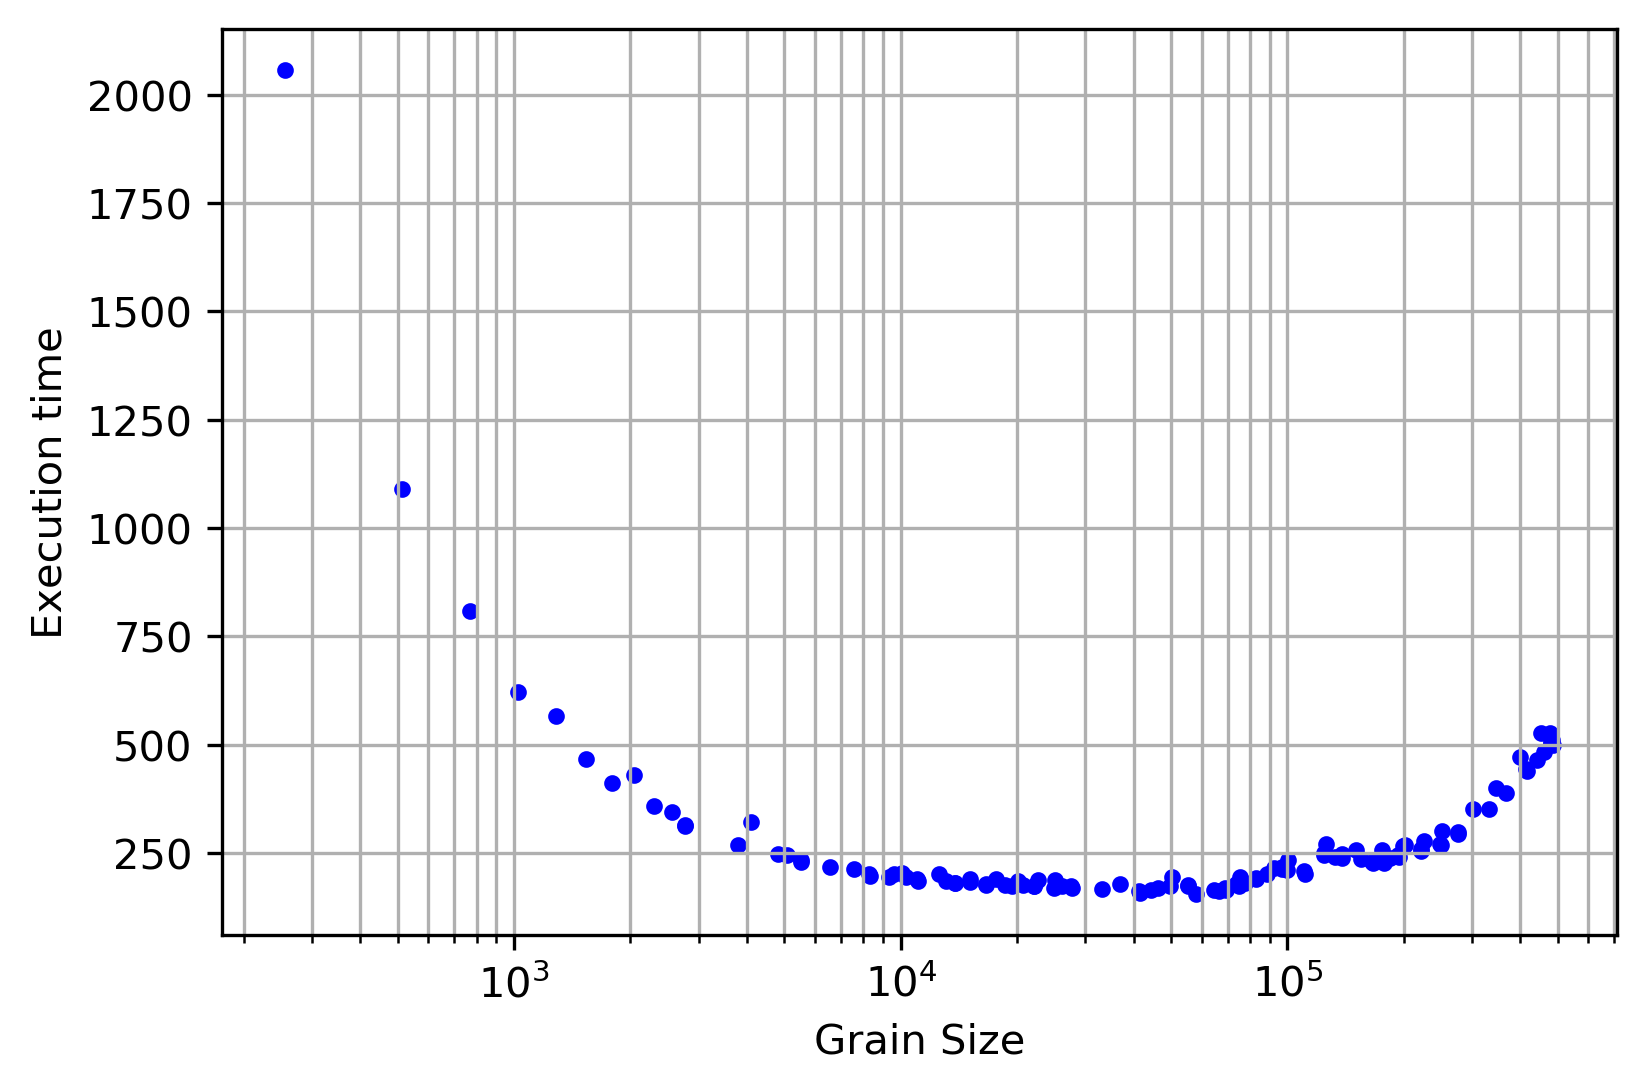
\includegraphics[scale=.3]{images/bathtub/all_690_4.png}\label{fig20:a}}
%	{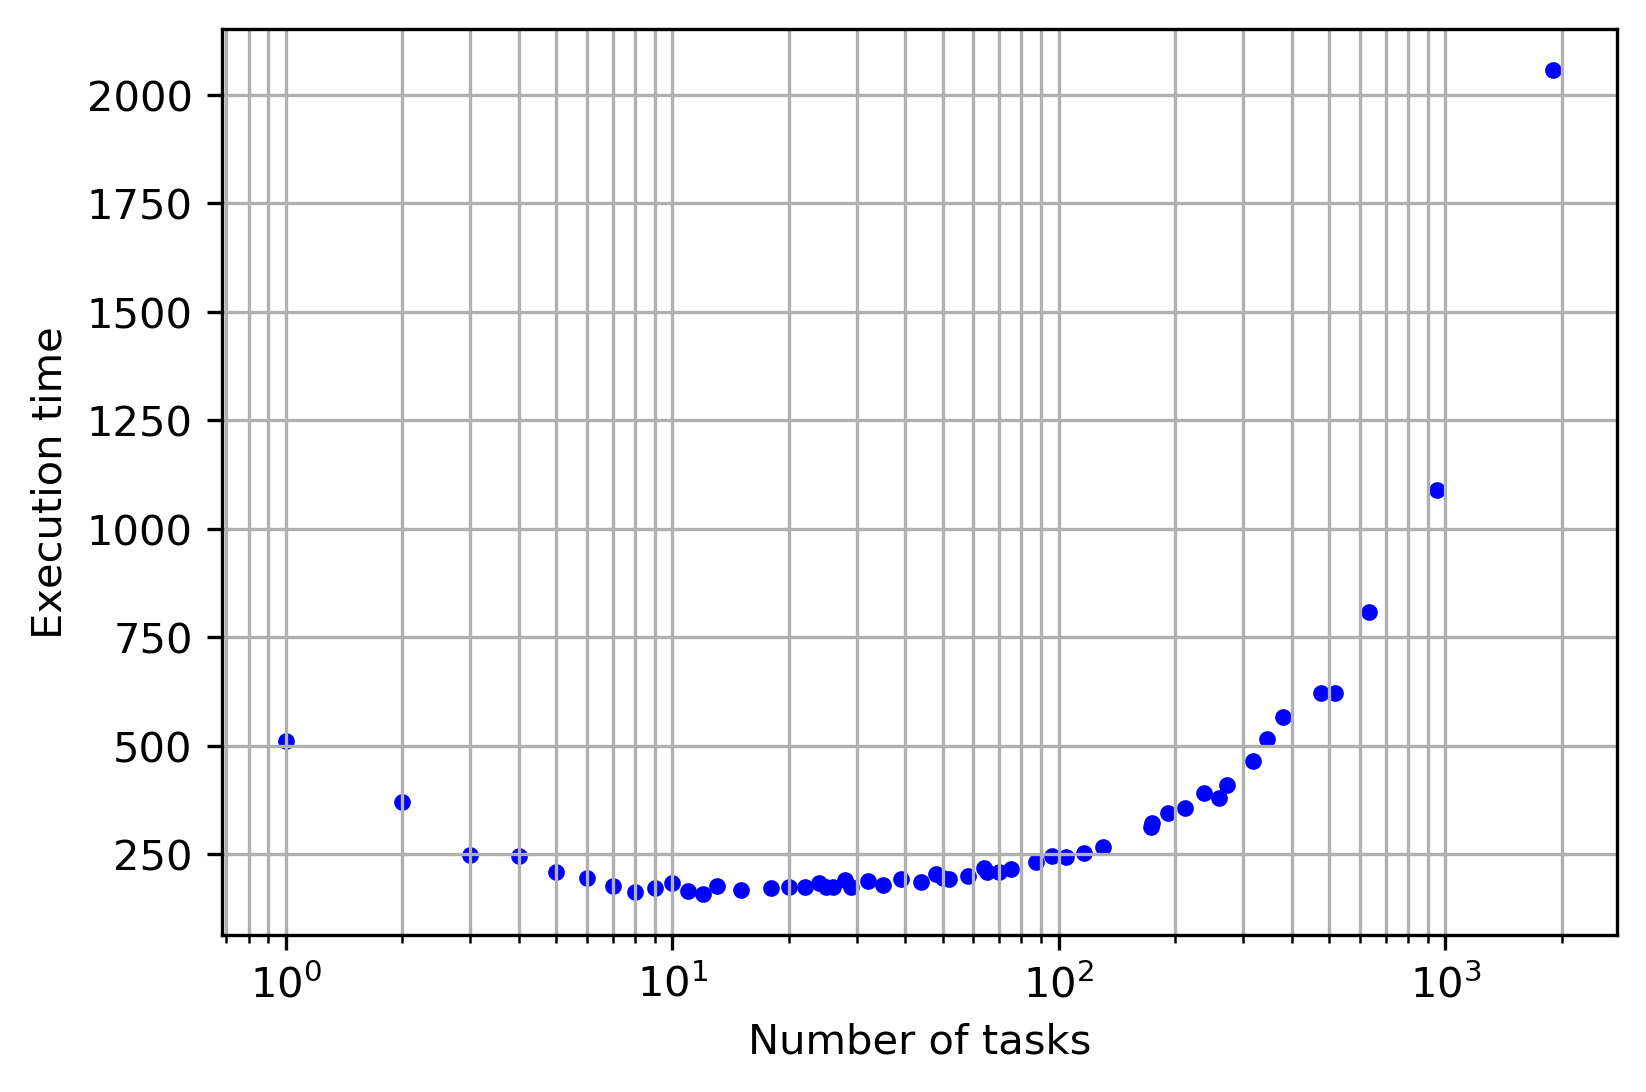
\includegraphics[scale=.3]{images/bathtub/tasks_all_690_4.png}\label{fig20:b}}
	\caption{The execution time vs. grain size graph for $DMATDMATADD$ benchmark for matrix size $690\times690$ ran on $4$ cores.}	
	\label{fig21}
\end{figure}
	\end{outline}
\end{frame}	


\begin{frame}{Modeling Execution Time based on Grain Size}
	\begin{outline}		
		\1Overheads of creating tasks
		\1Starvation
		\begin{figure}
			
			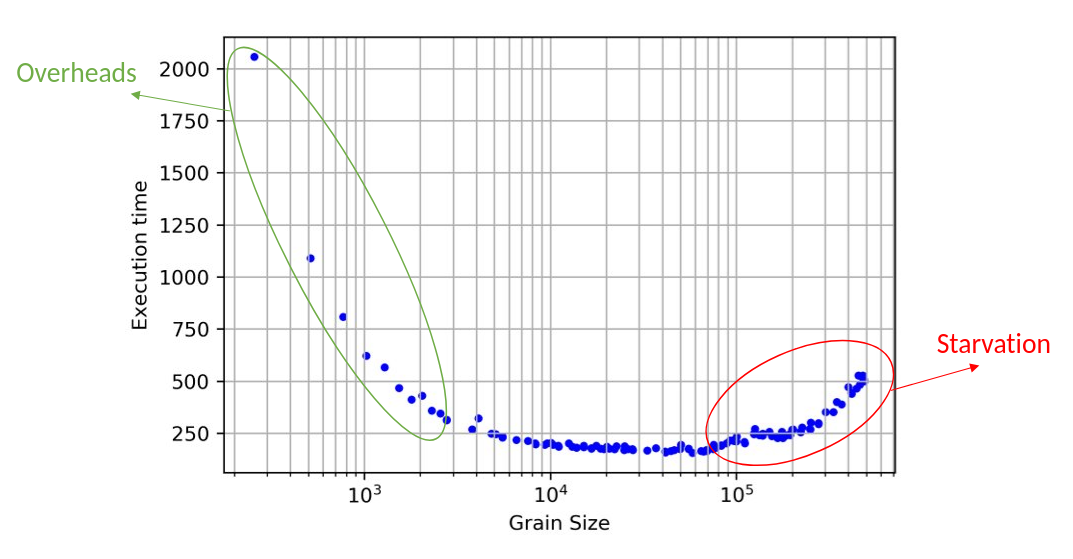
\includegraphics[width=0.9\linewidth]{images/bathtub/all_690_4_star_over.png}	
			\caption{Results of running the \textit{DMATDMATADD} benchmark on $8$ cores matrix size $690\times690$(time unit is microseconds)}	
		\end{figure}
	\end{outline}
\end{frame}

\begin{frame}{Modeling Execution Time based on Grain Size}
\begin{outline}		
	$$t=\left\{
	\begin{aligned}
		\alpha+\frac{t_s}{n_t}+\gamma  \:\:\:\:\:\:\:\:      \text{ if } n_t<N\\
		\frac{\alpha{n_t}+t_s}{N}+\gamma\:\:\:\:\:\:\:\:     \text{otherwise}
	\end{aligned}
	\right.$$

	$$n_t \text{: number of tasks}	$$
	$$N\text{: number of cores}$$
	$$t_s\text{: sequential execution time}$$
	$$\gamma\text{: parallelization constant}$$
%	Softplus function:
%	$$f(x)=Ln(1+e^x)$$

\end{outline}
\end{frame}

\begin{frame}{Modeling Execution Time based on Grain Size}
\begin{outline}	
	\1Fixed matrix size, and number of cores	
	\1Training set and test set (\%60, \%40)
	\begin{figure}[H]
		\centering
		{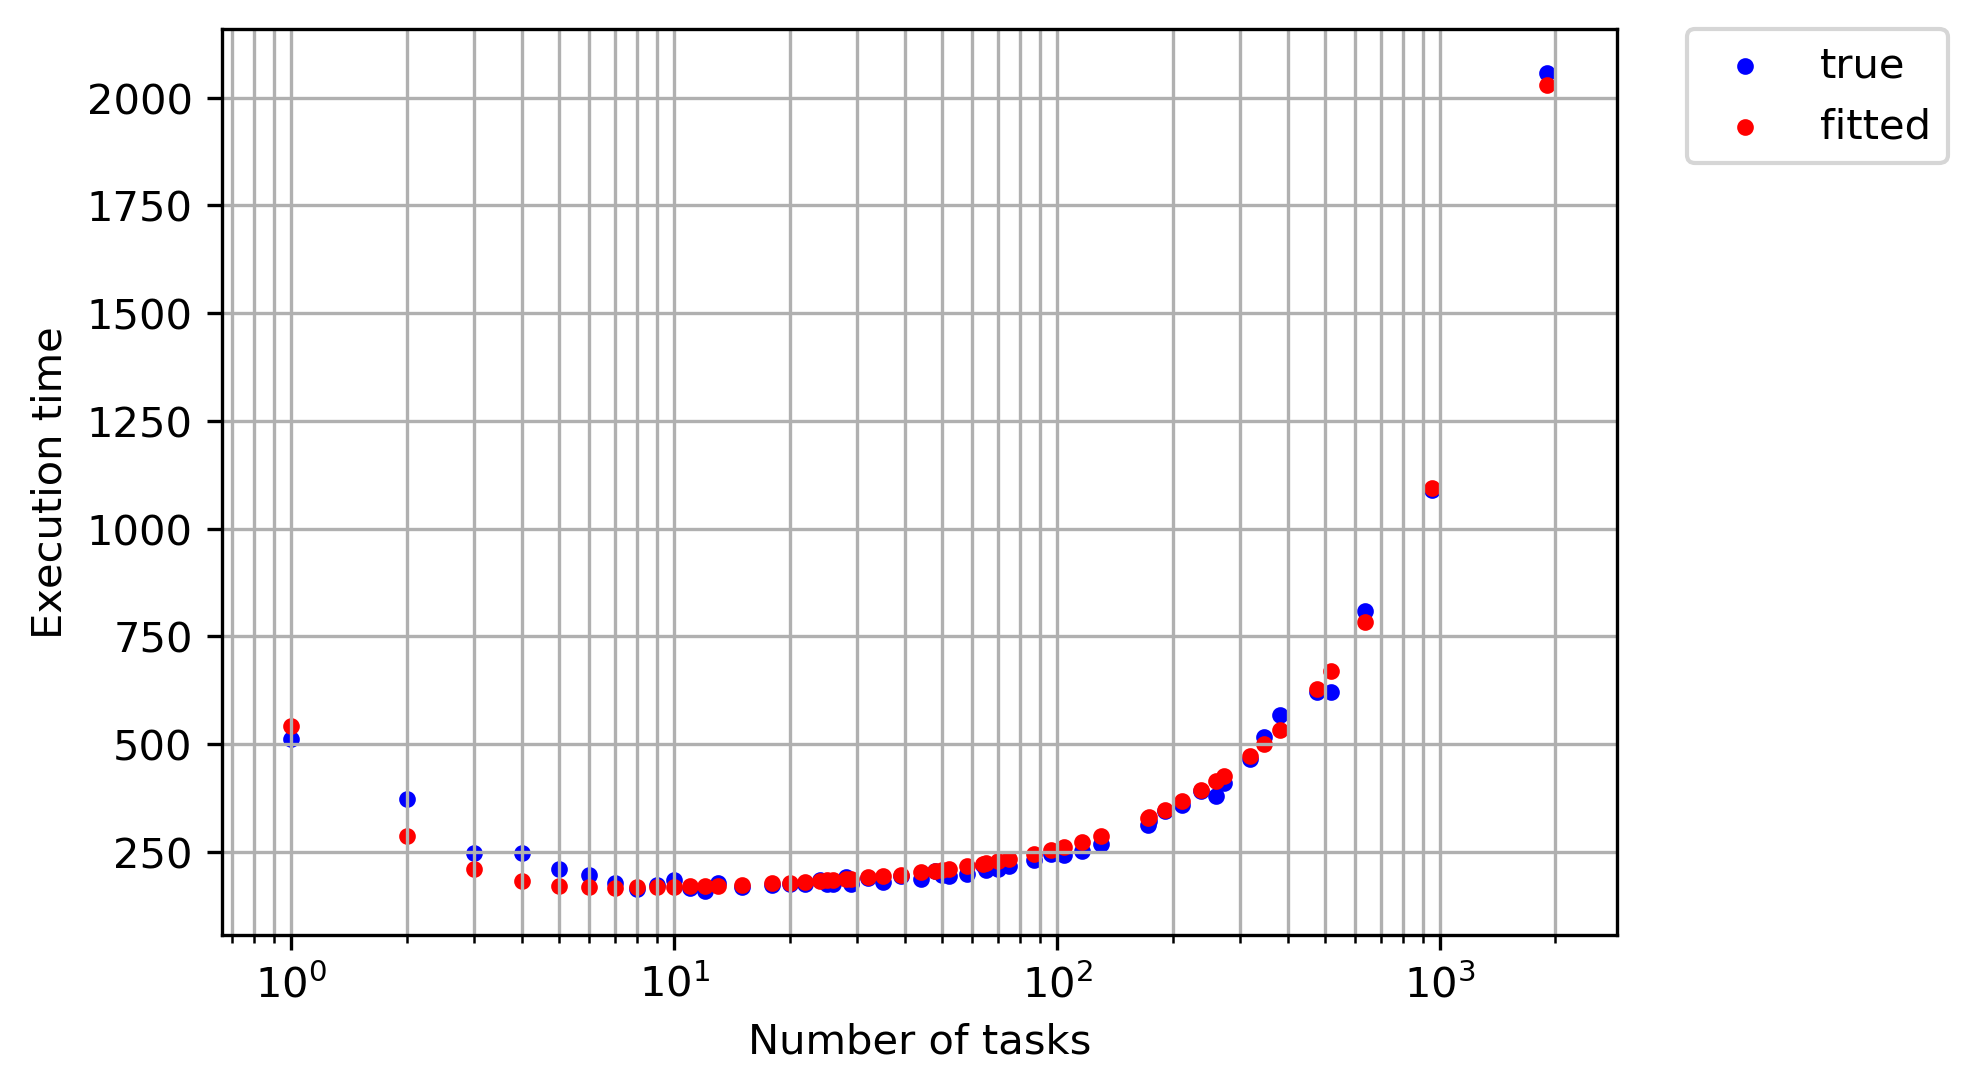
\includegraphics[scale=.4]{images/bathtub/pred/pred_690_4.png}\label{fig22:a}}
		{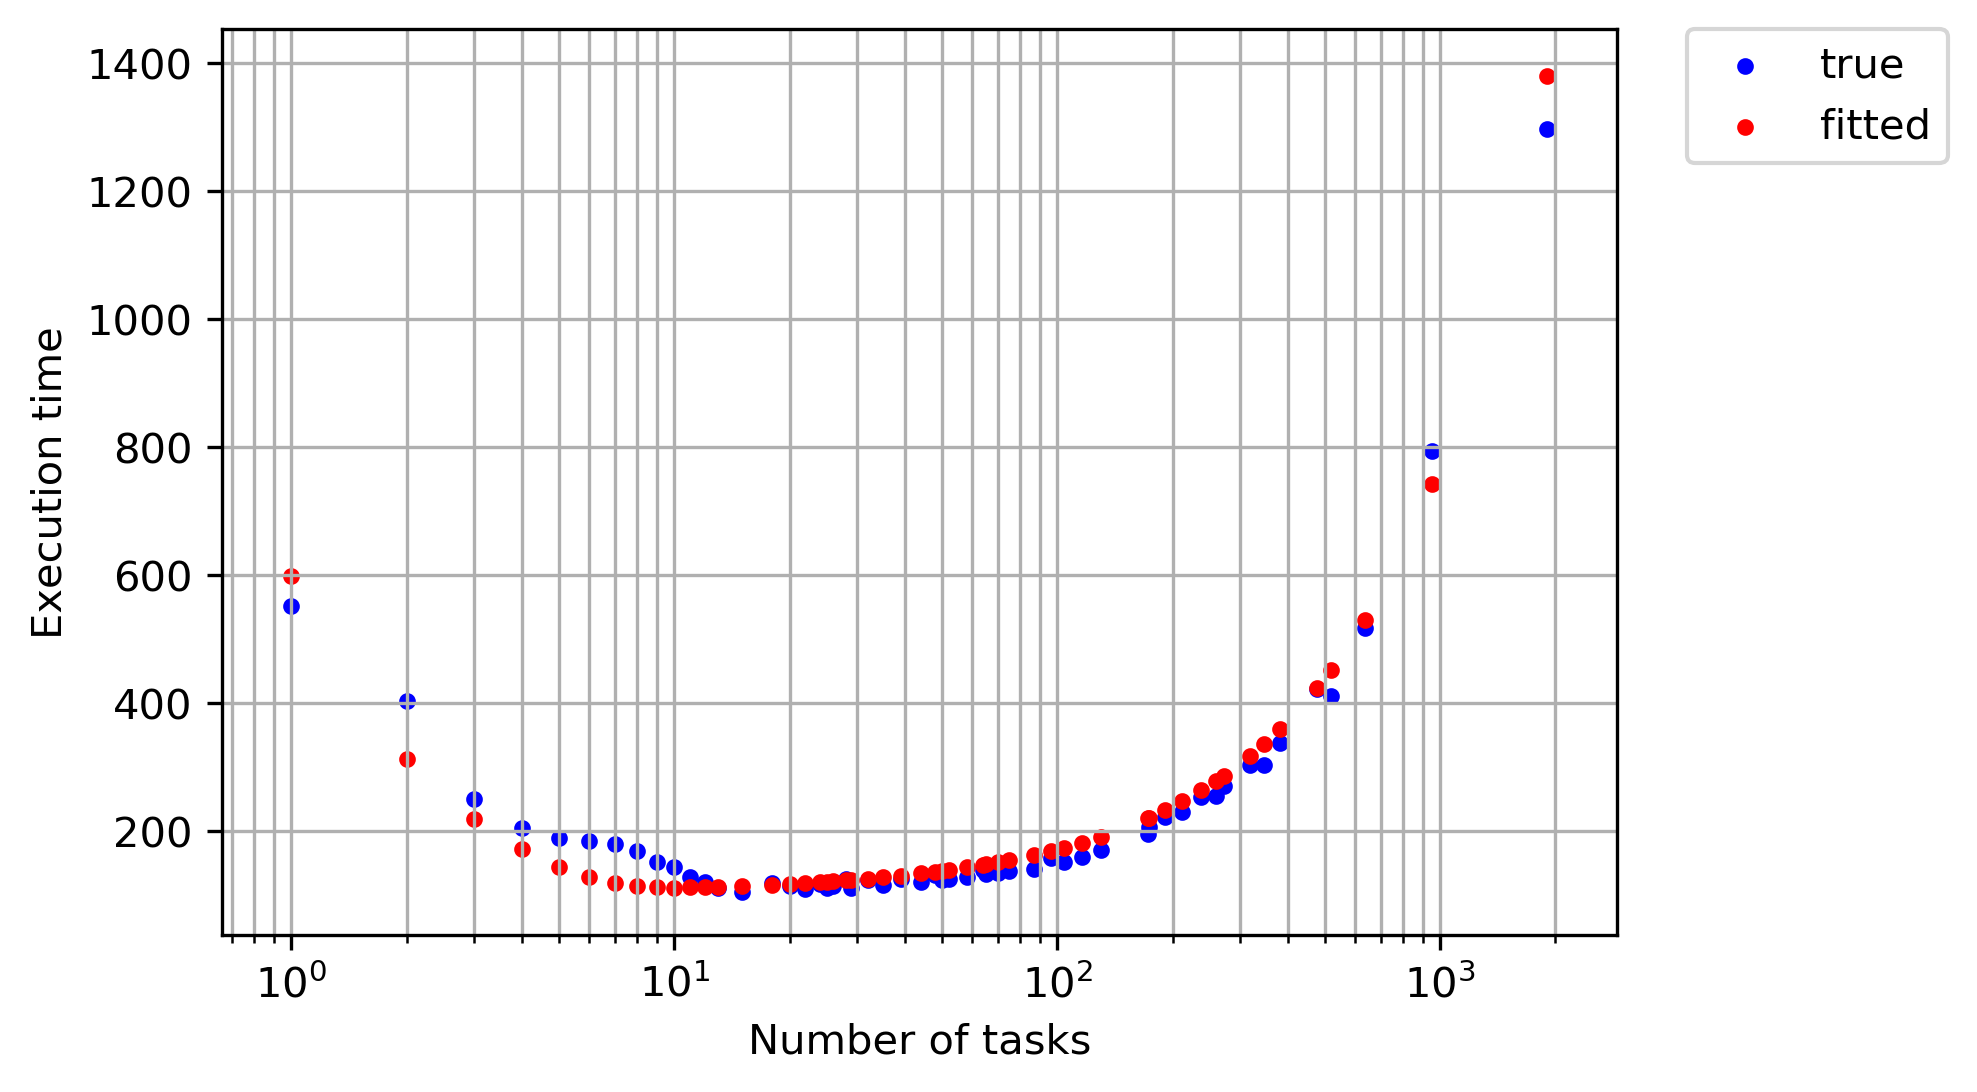
\includegraphics[scale=.4]{images/bathtub/pred/pred_690_8.png}\label{fig22:b}}	
		\caption{The prediction of execution time based on grain size using the bathtub model, for (a)4 cores and (b)8 cores for $DMATDMATADD$ benchmark for matrix size $690\times690$.}	
		\label{fig22}
	\end{figure}
\end{outline}
\end{frame}

\begin{frame}{Modeling Execution Time based on Grain Size}
	\begin{outline}	
\begin{figure}[H]
	\centering
	{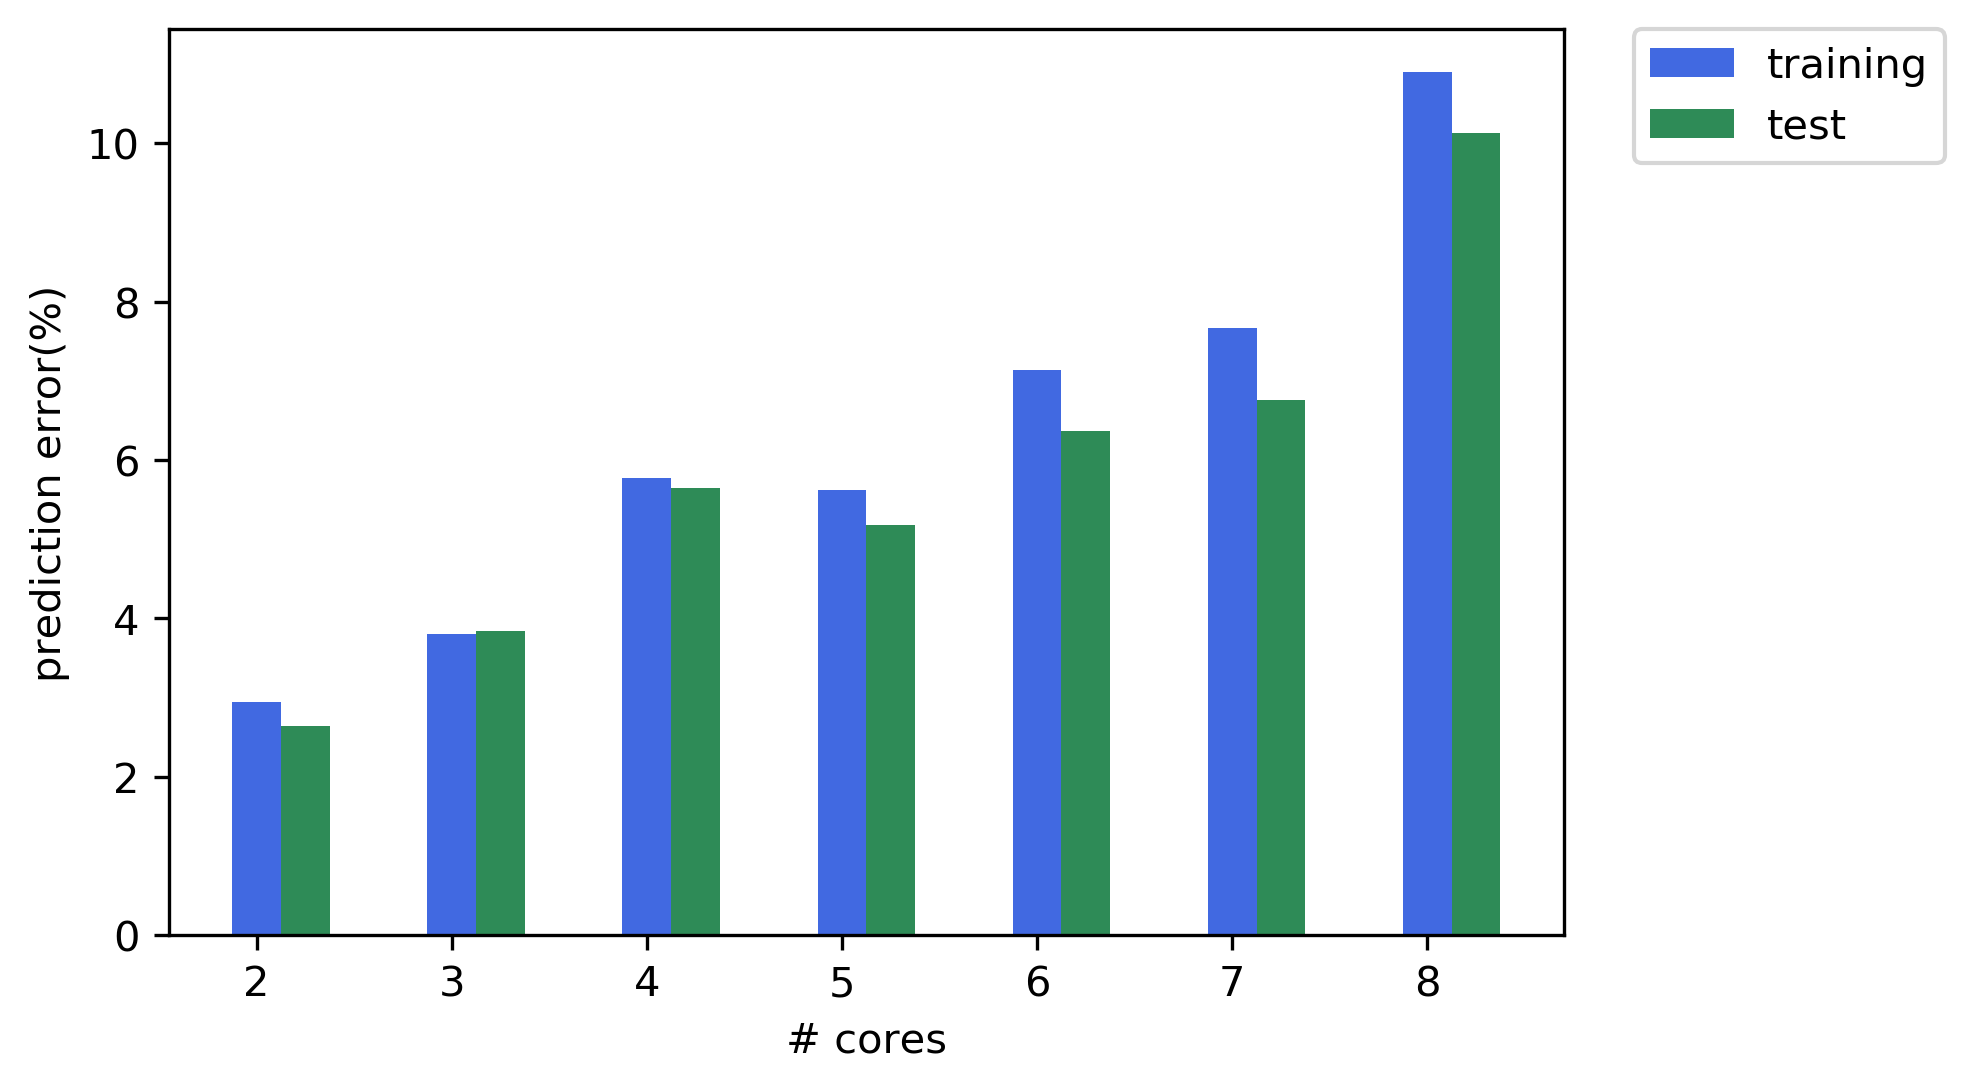
\includegraphics[scale=.45]{images/bathtub/error_690.png}}	
	\caption{The error in fitting execution time with the bathtub formula for $DMATDMATADD$ benchmark for matrix size $690\times690$ with different number of cores.}	
	\label{fig23}
\end{figure}
\end{outline}
\end{frame}

\begin{frame}{Modeling Execution Time based on Grain Size}
	\begin{outline}	
	How do $\alpha$, $t_s$, and $\gamma$ change with number of cores?	
	\begin{figure}[H]
		\centering
		{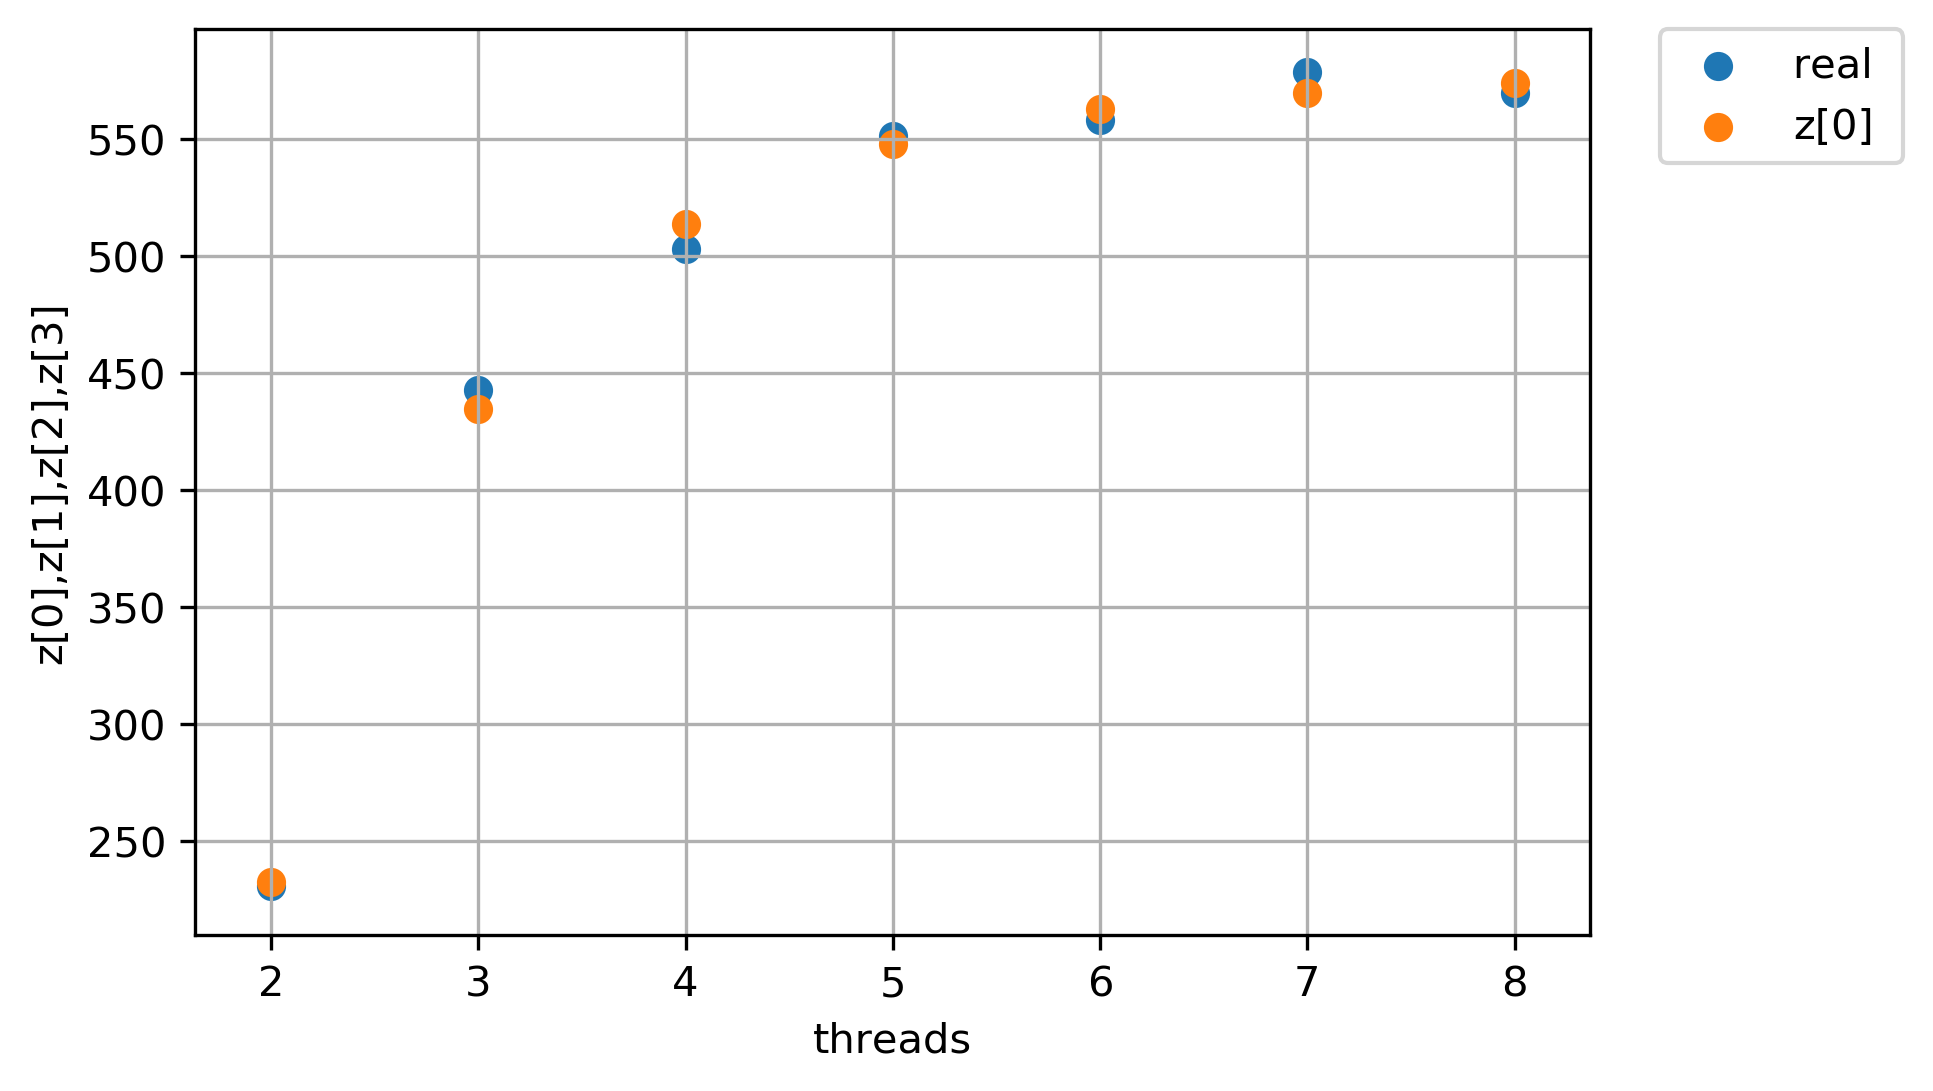
\includegraphics[scale=.3]{images/bathtub/coef_1_690.png}\label{fig24:a}}
		{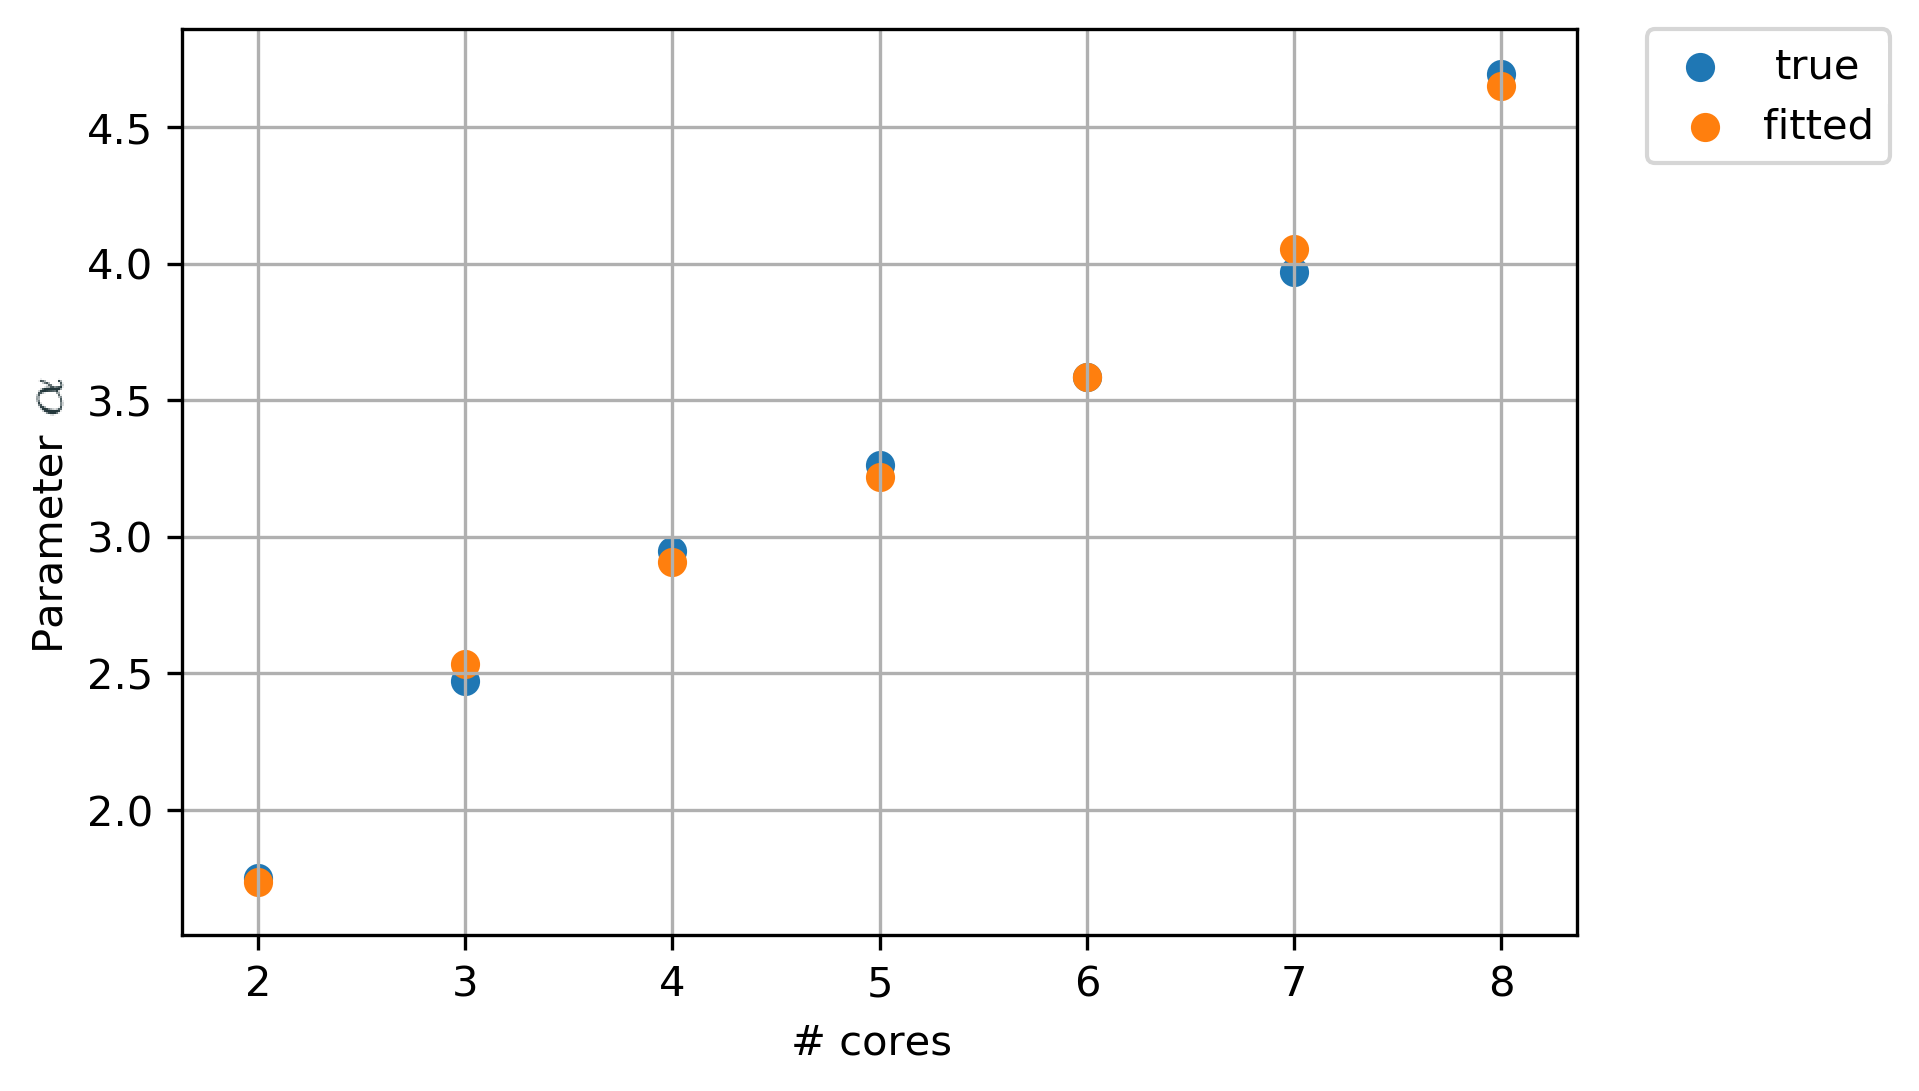
\includegraphics[scale=.3]{images/bathtub/coef_2_690.png}\label{fig24:b}}	
		{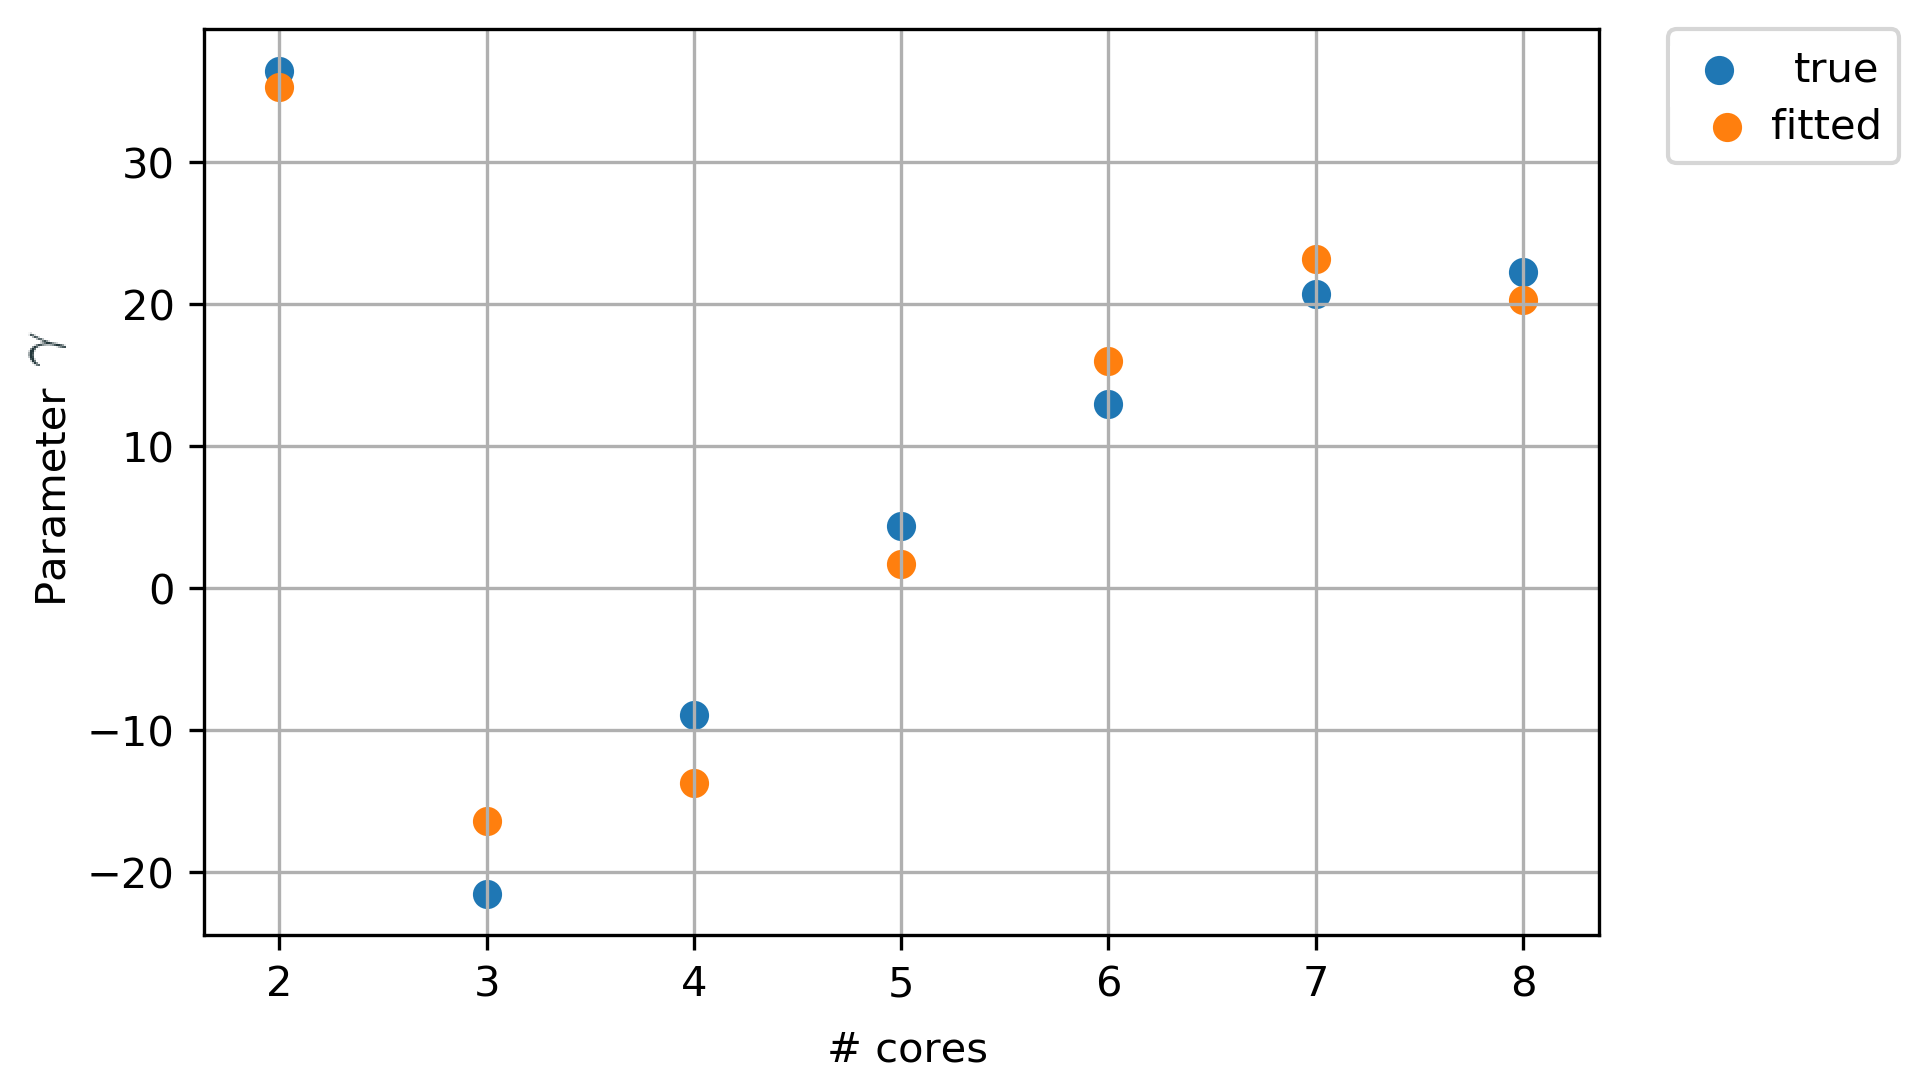
\includegraphics[scale=.3]{images/bathtub/coef_3_690.png}\label{fig24:c}}
		\caption{Fitting the three parameters (a)$\alpha$, (b)$t_s$, and (c)$\gamma$ for $DMATDMATADD$ benchmark for matrix size $690\times690$.}	
		\label{fig24}
	\end{figure}
	
	
$$f(x)=\frac{m_0}{x}+\frac{m_1(x-1)}{x}+m_2(x-1)+m_3(x)(x-1)$$
\end{outline}
\end{frame}


\begin{frame}{Modeling Execution Time based on Grain Size}
	\begin{outline}	
\begin{figure}[H]
	\centering	{\hfill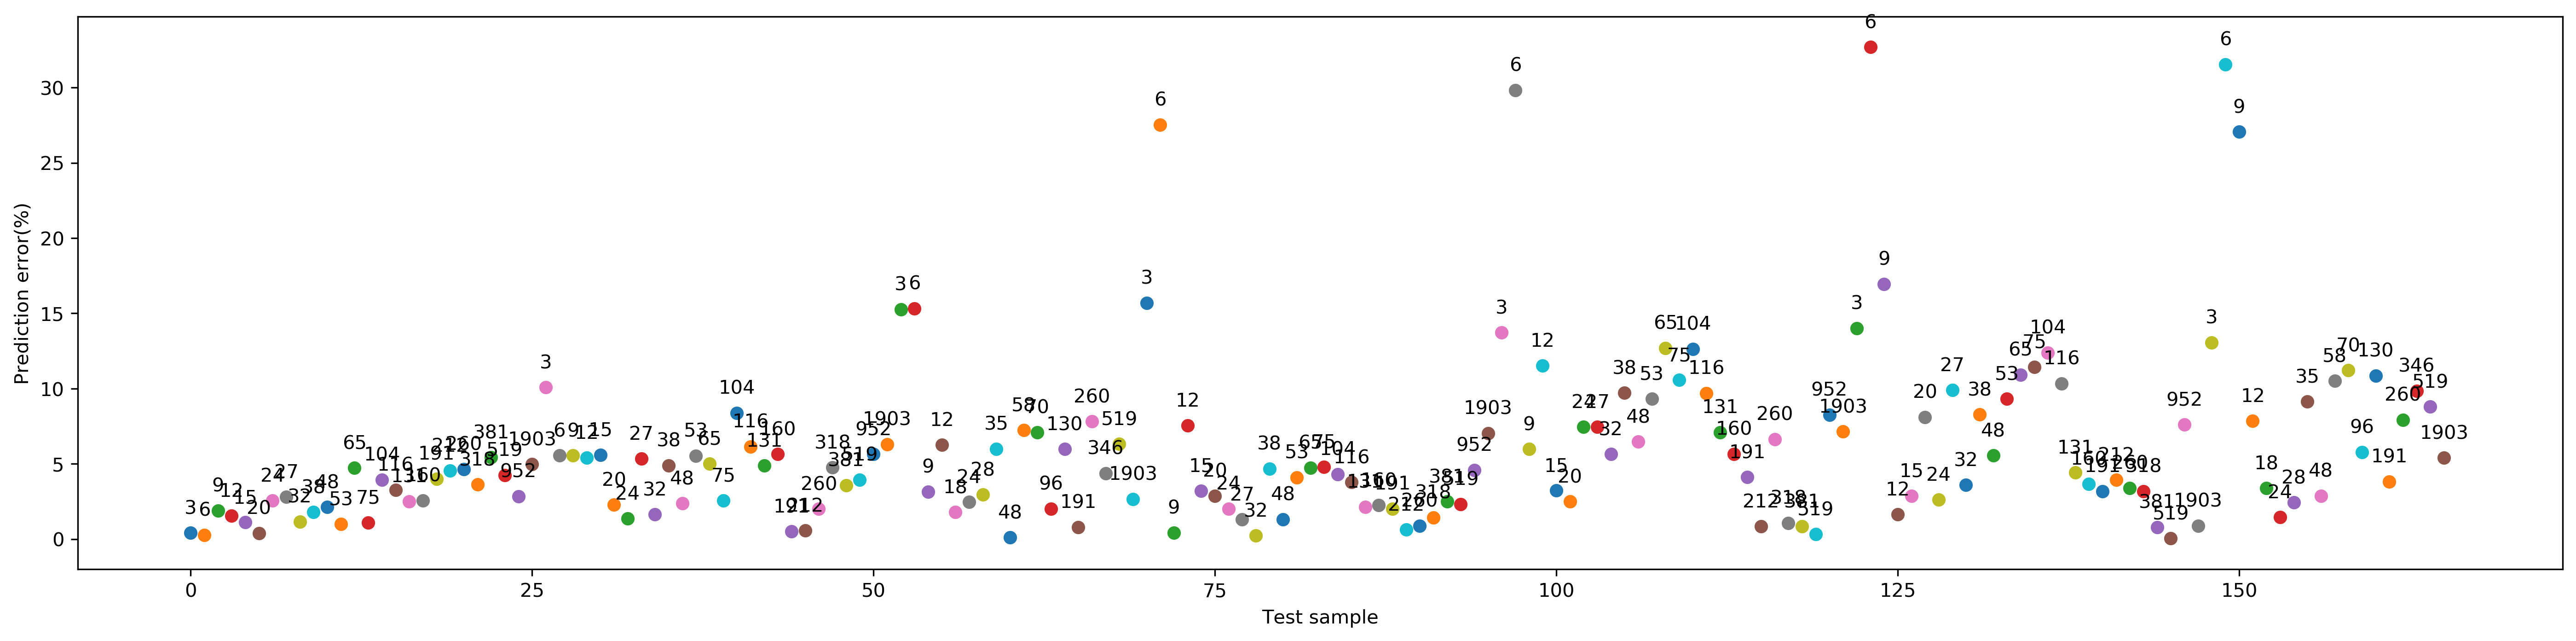
\includegraphics[scale=.25]{images/bathtub/prediction_error_overall690.png}}	
	\caption{The error in fitting execution time with the bathtub formula for $DMATDMATADD$ benchmark for matrix size $690\times690$ with different number of cores.}	
	\label{fig25}
\end{figure}
\end{outline}
\end{frame}

\begin{frame}{Modeling Execution Time based on Grain Size}
	\begin{outline}	
The problem with the current model is that with this formula we know that the minimum occurs at $n_t=N$.

\end{outline}
\end{frame}


%\begin{frame}{Modeling Execution Time based on Grain Size}
%\begin{outline}	
%	\1For a fixed matrix size, and number of cores we need 4 parameters to estimate execution time based on number of tasks
%    \1How does these four parameters change for different number of cores?
%    \2used USL to model each of these parameters
%\end{outline}
%\end{frame}



%\section{Setup}
\begin{frame}{Setup: Blazemark}
	\begin{outline}
		Blazemark is a benchmark suite provided by Blaze to compare the performance of Blaze with other linear algebra libraries. 
		\begin{figure}
			\includegraphics[width=0.42\linewidth]{images/blazemark_1.png}
			\hfill\includegraphics[width=0.41\linewidth]{images/blazemark_2.png}
			\caption{An example of results obtained from Blazemark}	
		\end{figure}
	\end{outline}
\end{frame}


\begin{frame}{Setup: Configuration}
	\begin{outline}
	\vspace{\baselineskip}	
	\begin{table}[H]
		\centering
		%	\resizebox{\textwidth}{!}
		\scalebox{0.75}
		{\begin{tabular}{|c | c |} 
				\hline
				
				Category & Specification\\
				\hline
				\hline
				CPU &  2 x Intel(R) Xeon(R) CPU E5-2450 0 @ 2.10GHz \\ [0.5ex] 
				\hline
				RAM & 48 GB\\ 	
				\hline
				Number of Cores & 16\\
				\hline	
				Hyperthreading & Off \\
				\hline			
		\end{tabular}}	
		\caption{Specifications of the Marvin node from Rostam cluster at CCT.}
		\label{table3}
	\end{table} 
\begin{table}[H]
	\centering
	%	\resizebox{\textwidth}{!}
	\scalebox{0.75}
	{\begin{tabular}{|c | c |} 
			\hline
			Library & Version \\
			\hline
			\hline
			HPX & 1.3.0 \\ 
			\hline
			Blaze & 3.5\\ 	
			\hline
			
	\end{tabular}}	
	\caption{Specifications of the libraries used to run our experiments.}
	\label{table5}
\end{table}
	\end{outline}
\end{frame}

\section{Related Work}
	\begin{frame}{Related Work}
		\begin{outline}
			\1Estimating the optimal number of cores to run the program on
			\1Zahra Used logostic regsression to find the best chunk size
			\1Gabriel Used machine learning to find the best chunk size, while block size was fixed statically
			\1Peter thoman proposed a compile-time and runtime solution 
		\end{outline}
\end{frame}



\section{Proposed Study}
\begin{frame}{Proposed Study}
\begin{outline}	
	\begin{figure}[H]
		\centering
		\includegraphics[scale=.25]{images/polyfit/fig_523-912_peak_range_all.png}
		\includegraphics[scale=.25]{images/fig11.png}	
		\label{fig20}
	\end{figure} 
	\1Studying the bathtub model
	\1Generalization for matrix size 
	\1Adding runs for larger matrix sizes
	\1Generalization for complex expressions
	\1Generalization for different architectures
\end{outline}
\end{frame}


\begin{frame}[standout]
  Thank you!
\end{frame}

\end{document}
